%%%%%%%%%%%%%%%%%%%%%%%%%%%%%%%%%%%%%%%%%%%%%%%%%%%%%%%%%%%%%%%%%%%%%%%%%%%%%%%%
%                         FORMATO DE TESIS UMSNH                               %
%%%%%%%%%%%%%%%%%%%%%%%%%%%%%%%%%%%%%%%%%%%%%%%%%%%%%%%%%%%%%%%%%%%%%%%%%%%%%%%%
% based on Harish Bhanderi's PhD/MPhil template, then Uni Cambridge
% http://www-h.eng.cam.ac.uk/help/tpl/textprocessing/ThesisStyle/
% corrected and extended in 2007 by Jakob Suckale, then MPI-iCBG PhD programme
% and made available through OpenWetWare.org - the free biology wiki
% forked from https://github.com/Tepexic/Tesis-UNAM on July 2017
% modifications made by Arturo Lopez Pineda

%                     Under GNU License v3

% ADAPTADO PARA UMSNH:  @arturolp

\documentclass[twoside,11pt]{Latex/Classes/thesisUMSNH}
%         PUEDEN INCLUIR EN ESTE ESPACIO LOS PAQUETES EXTRA, O BIEN, EN EL ARCHIVO "PhDthesisPSnPDF.cls" EN "./Latex/Classes/"
\usepackage{blindtext}                        % Para insertar texto dummy, de ejemplo, pues.
\usepackage[sort, numbers]{natbib}    % Personalizar la bibliografía a gusto de cada quien
\usepackage{url}

\usepackage{multirow}
\usepackage{tcolorbox}
\usepackage{amsmath}
% Note:
% The \blindtext or \Blindtext commands throughout this template generate dummy text
% to fill the template out. These commands should all be removed when 
% writing thesis content.
% This file contains macros that can be called up from connected TeX files
% It helps to summarise repeated code, e.g. figure insertion (see below).

%%%%%%%%%%%%%%%%%%%%%%%%%%%%%%%%%%%%%%%%%%%%%%
%            Colores de la UNAM              %
%%%%%%%%%%%%%%%%%%%%%%%%%%%%%%%%%%%%%%%%%%%%%%
% Para UNAN: Azul Pantone 541  -->(0,63,119) RGB
% Para UMSNH: PANTONE Blue 072 C
\definecolor{Azul}{RGB}{51,51,153}

% Para UNAM: Oro Pantone 460  -->(234,221,150) RGB
% Para UMNSH: PANTONE 110 C
\definecolor{Oro}{RGB}{204,153,51}


%%%%%%%%%%%%%%%%%%%%%%%%%%%%%%%%%%%%%%%%%%%%%%
%            Comandos para líneas            %
%%%%%%%%%%%%%%%%%%%%%%%%%%%%%%%%%%%%%%%%%%%%%%
%Se define un comando \colorvrule para hacer líneas verticales de color con 3 argumentos: color, ancho, alto
\newcommand{\colorvrule}[3]{
\begingroup\color{#1}\vrule width#2 height#3
\endgroup}

%Se define un comando \colorhrule para hacer líneas horizontales de color con 2 argumentos: color, ancho
\newcommand{\colorhrule}[2]{
\begingroup\color{#1}\hrule height#2
\endgroup}

%%%%%%%%%%%%%%%%%%%%%%%%%%%%%%%%%%%%%%%%%%%%%%
%          Comando para derivadas            %
%%%%%%%%%%%%%%%%%%%%%%%%%%%%%%%%%%%%%%%%%%%%%%
\newcommand{\derivada}[3][]{\ensuremath{\dfrac{\mbox{d}^{#1}#2}{\mbox{d}#3^{#1}}}} 
%primer argumento(opcional): orden de la derivada
%segundo argumento: función a derivar
%tercer argumento: variable respecto a la que se deriva


%%%%%%%%%%%%%%%%%%%%%%%%%%%%%%%%%%%%%%%%%%%%%%
%       Comando para la exponencial          %
%%%%%%%%%%%%%%%%%%%%%%%%%%%%%%%%%%%%%%%%%%%%%%
\newcommand{\e}[1][]{\ensuremath{\mbox{e}^{#1}}}
%primer argumento(opcional): exponente de la exponencial




% insert a centered figure with caption and description
% parameters 1:filename, 2:title, 3:description and label
\newcommand{\figuremacro}[3]{
	\begin{figure}[htbp]
		\centering
		\includegraphics[width=1\textwidth]{#1}
		\caption[#2]{\textbf{#2} - #3}
		\label{condicion}
	\end{figure}
}

% insert a centered figure with caption and description AND WIDTH
% parameters 1:filename, 2:title, 3:description and label, 4: textwidth
% textwidth 1 means as text, 0.5 means half the width of the text
\newcommand{\figuremacroW}[4]{
	\begin{figure}[htbp]
		\centering
		\includegraphics[width=#4\textwidth]{#1}
		\caption[#2]{\textbf{#2} - #3}
		\label{#1}
	\end{figure}
}

% inserts a figure with wrapped around text; only suitable for NARROW figs
% o is for outside on a double paged document; others: l, r, i(inside)
% text and figure will each be half of the document width
% note: long captions often crash with adjacent content; take care
% in general: above 2 macro produce more reliable layout
\newcommand{\figuremacroN}[3]{
	\begin{wrapfigure}{o}{0.5\textwidth}
		\centering
		\includegraphics[width=0.48\textwidth]{#1}
		\caption[#2]{{\small\textbf{#2} - #3}}
		\label{#1}
	\end{wrapfigure}
}

% predefined commands by Harish
\newcommand{\PdfPsText}[2]{
  \ifpdf
     #1
  \else
     #2
  \fi
}

\newcommand{\IncludeGraphicsH}[3]{
  \PdfPsText{\includegraphics[height=#2]{#1}}{\includegraphics[bb = #3, height=#2]{#1}}
}

\newcommand{\IncludeGraphicsW}[3]{
  \PdfPsText{\includegraphics[width=#2]{#1}}{\includegraphics[bb = #3, width=#2]{#1}}
}

\newcommand{\InsertFig}[3]{
  \begin{figure}[!htbp]
    \begin{center}
      \leavevmode
      #1
      \caption{#2}
      \label{#3}
    \end{center}
  \end{figure}
}







%%% Local Variables:
%%% mode: latex
%%% TeX-master: "~/Documents/LaTeX/CUEDThesisPSnPDF/thesis"
%%% End:
           % Archivo con funciones útiles
\usepackage[draft,inline,nomargin]{fixme} \fxsetup{theme=color}
\FXRegisterAuthor{cp}{cfp}{\color{blue}Carlos}
\FXRegisterAuthor{jm}{jmb}{\color{red}Josué}



\graphicspath{{images/},{figures/}}

\usepackage{lineno}
\linenumbers

%%%%%%%%%%%%%%%%%%%%%%%%%%%%%%%%%%%%%%%%%%%%%%%%%%%%%%%%%%%%%%%%%%%%%%%%%%%%%%%%
%                                   DATOS                                      %
%%%%%%%%%%%%%%%%%%%%%%%%%%%%%%%%%%%%%%%%%%%%%%%%%%%%%%%%%%%%%%%%%%%%%%%%%%%%%%%%
\title{Análisis estadístico del flujo de 1-gramas entre lenguajes indoeuropeos}
\author{JOSUÉ ELY MOLINA BECERRA} 
\facultad{FACULTAD DE CIENCIAS}                 % Nombre de la facultad/escuela
\escudofacultad{Latex/Classes/Escudos/fc_negro.pdf} % Aquí ponen la ruta y nombre del escudo de su facultad, actualmente, la carpeta Latex/Classes/Escudos cuenta con los siguientes escudos:
% "fi_azul" Facultad de ingenieria en color azul
% "fi_negro" Facultad de ingenieria en color negro
% "fc_azul" Facultad de ciencias en color azul
% "fc_negro" Facultad de ciencias en color negro
% Se agradecen sus aportaciones de escudos a jebus.velazquez@gmail.com

\degree{FÍSICO}       % Carrera
\director{CARLOS FRANCISCO PINEDA ZORRILLA}                   % Director de tesis
%\tutor{Nombre  Tutor }                    % Tutor de tesis, si aplica
\degreedate{2019}                                     % Año de la fecha del examen
\lugar{CIUDAD DE MÉXICO}                        % Lugar

\portadafalse                              % Portada en NEGRO, descomentar y comentar la línea siguiente si se quiere utilizar
%\portadatrue                                % Portada en COLOR



%% Opciones del posgrado (descomentar si las necesitan)
	%\posgradotrue                                                    
	%\programa{programa de maestría y doctorado en ingeniería}
	%\campo{Ingeniería Eléctrica - Control}
	%% En caso de que haya comité tutor
	%\comitetrue
	%\ctutoruno{Dr. Emmet L. Brown}
	%\ctutordos{Dr. El Doctor}
%% Datos del jurado                             
	%\presidente{Dr. 1}
	%\secretario{Dr. 2}
	%\vocal{Dr. 3}
	%\supuno{Dr. 4}
	%\supdos{Dr. 5}
	%\institucion{el Instituto de Ingeniería, UNAM}

\keywords{tesis,autor,tutor,etc}            % Palablas clave para los metadatos del PDF
\subject{tema_1,tema_2}                     % Tema para metadatos del PDF  

%%%%%%%%%%%%%%%%%%%%%%%%%%%%%%%%%%%%%%%%%%%%%%%%%%%%%
%                   PORTADA                         %
%%%%%%%%%%%%%%%%%%%%%%%%%%%%%%%%%%%%%%%%%%%%%%%%%%%%%
\begin{document}

\maketitle									% Se redefinió este comando en el archivo de la clase para generar automáticamente la portada a partir de los datos

%%%%%%%%%%%%%%%%%%%%%%%%%%%%%%%%%%%%%%%%%%%%%%%%%%%%%
%                  PRÓLOGO                          %
%%%%%%%%%%%%%%%%%%%%%%%%%%%%%%%%%%%%%%%%%%%%%%%%%%%%%
\frontmatter
\begin{acknowledgementspersonal}
	
Principalmente a mi abuela Nieves, por haberme cuidado y procurado tantos años sin ser su responsabilidad. 

\vspace{0.5cm}
A mis tios, padrinos y en muchas ocasiones mis padres, Dolores y Oscar; mis primas Flor y Yoalli, también Yurai. Gracias por apoyarme, aceptarme y darme una convivencia familiar.

\vspace{0.5cm}
A mi madre María de la Luz, por darme en mi niñez el aprecio a los libros y a la lectura; y porque en los últimos años, con su desinterés y su desconfianza, me enseñó a sólo depender en mi mismo. 

\vspace{0.5cm}
A mis primos Román, Alfonso y Sinar, por mostrarme que el trabajo duro nos lleva más lejos de la realidad donde nos toco nacer. 

\vspace{0.5cm}
A mi familia paterna, mis primos Liz, Carlos, Griss, Sandy, Elias, Martha y Yadi; mis tias Paty, Cata, Lupe y Xila; y a toda la \textit{Molinada sin fin}, por aceptarme dentro de una gran familia y por ayudarme a cumplir mi deseo.  

\vspace{0.5cm}
A Pamela, Diego, Zoé, Hilary y Yultzín, por ser mi mejor recuerdo de Fundación;  a Maffer, Cabral, Gaby y Alejandro por los \textit{buenos aires} del primer año de preparatoria; a Mauricio, Charly y Alex Califas por los mejores días en las canchas y en \textit{Potrero Dome}; a Brenda, Hodek y Kas \textit{Panda} por las platicas de humanidades, artes, historia y filosofía.  

\vspace{0.5cm}
Nuevamente a Pamela, Zoé, Maffer, Cabral, Mauricio y Charly, porque ustedes se han vuelto más que mis mejores amigos, gracias a ustedes y a sus familias por lo vivido y lo aprendido.

\vspace{0.5cm}
A Carla, por los años en la universidad en los que me mostró amistad, cariño y comprensión; por enseñarme a trabajar en equipo y también por llevarme a \textit{lo más alto y lo más bajo}.

\vspace{0.5cm}
A mis hermanos Carlos, Pavlos, George y Jack,  y a mi hermana Aila, porque ustedes son el mejor regalo y la mejor ilusión que el tiempo me brindó, y porque su existencia es la motivación para cruzar el mundo.

\vspace{0.5cm}
Finalmente a mi padre Carlos Molina Jiménez, porque su ausencia y su ejemplo, me hicieron ver que la formación académica no lo es todo,  y a la vez es la camino para superarnos y llegar a lo más alto. 


\end{acknowledgementspersonal}       % Comentar línea si no se usa
%\chapter*{}
%\pagenumbering{Roman}

\begin{acknowledgementsacademic}

Gracias a la UNAM por la formación académica recibida, y por el ejemplo profesional que me brindó en su personal, en la Preparatoria 9 con los profesores Norma Ramírez, Patricia Huerta, Elsa Cano, Arturo Palafox, José Carbajal y Arturo Jiménez; y en la Facultad de Ciencias con  Rosario Paredes, Patricia Goldstein, Pablo Barrera, Mirna Villavicencio, Valentín Porta, Ricardo Méndez, Roxana del Castillo y Catalina Stern. Gracias a todos por su labor, su ética y moral profesional,  y por todo el apoyo brindado. 

\vspace{0.5cm}
Gracias a todos los miembros del  grupo de idiomas, por formarme y enseñarme que se puede hacer física en las cosas más cotidianas, no sólo en los fenómenos abstractos. 

\vspace{0.5cm}
Gracias a mi asesor el Dr. Carlos Pineda, por sus consejos, su compresión, su apoyo y paciencia en las múltiples reuniones para elaborar este trabajo. También porque me enseño que en la ciencia,  lo más importante no son las formulaciones y los desarrollos complicados, sino la explicación y la sencillez con la que nos expresamos. 

\vspace{0.5cm}
Finalmente, gracias a los apoyos de los proyectos PAPIIT IG100518 y CONACYT CB-285754, ya que con ellos fue posible cada parte del desarrollo de está tesis. 

\end{acknowledgementsacademic}




   % Comentar línea si no se usa 
%% ******************************* Thesis Declaration ********************************

\begin{declaration}

Por la presente declaro que, salvo cuando se haga referencia específica al trabajo de otras personas, el contenido de esta tesis es original y no se ha presentado total o parcialmente para su consideración para cualquier otro título o grado en esta o cualquier otra Universidad. Esta tesis es resultado de mi propio trabajo y no incluye nada que sea el resultado de algún trabajo realizado en colaboración, salvo que se indique específicamente en el texto. 
% Author and date will be inserted automatically from thesis.tex


\end{declaration}
           % Comentar línea si no se usa

\begin{abstracts}        

En los últimos años, el desarrollo científico y tecnológico,  y el crecimiento económico de países como los Estados Unidos,  han hecho del idioma inglés el lenguaje común para la comunicación y para la difusión de información. Esto ha provocado que algunos vocablos del inglés comiencen a surgir en los demás idiomas,  mezclándose con las palabras típicas del idioma, y en ocasiones desplazándolas.  

Está tendencia no ha sido una característica única del inglés, a lo largo del tiempo, diferentes idiomas han aportado y modificado el vocabulario de otras lenguas. En este trabajo se estudia la forma en que los idiomas inglés, francés, alemán, italiano y español, se han relacionado durante el siglo XX a través de las palabras que son comunes entre ellos, llamadas  \textit{palabras migrantes};  y a partir de ellas, se han propuesto dos formas para cuantificar la influencia que un idioma ha tenido en otro. 

También se presenta un estudio estadístico llamado \textit{diversidad de rango}, con el que se cuantifican las distintas palabras migrantes que pueden ocupar lugar en un listado, si estas se ordenan  a partir de su frecuencia.  

Finalmente se justifica la falta de un rigor lingüístico, al eliminar cierta cantidad de palabras migrantes, para volver a obtener la influencia entre idiomas, y medir su similitud con los resultados previos. 



 
\end{abstracts}
%\end{abstractlongs}


% ----------------------------------------------------------------------                   % Comentar línea si no se usa

%%%%%%%%%%%%%%%%%%%%%%%%%%%%%%%%%%%%%%%%%%%%%%%%%%%%%
%                   ÍNDICES                         %
%%%%%%%%%%%%%%%%%%%%%%%%%%%%%%%%%%%%%%%%%%%%%%%%%%%%%
%Esta sección genera el índice
\setcounter{secnumdepth}{3} % organisational level that receives a numbers
\setcounter{tocdepth}{3}    % print table of contents for level 3
\tableofcontents            % Genera el índice 
%: ----------------------- list of figures/tables ------------------------
\listoffigures              % Genera el ínidce de figuras, comentar línea si no se usa
\listoftables               % Genera índice de tablas, comentar línea si no se usa


%%%%%%%%%%%%%%%%%%%%%%%%%%%%%%%%%%%%%%%%%%%%%%%%%%%%%
%                   CONTENIDO                       %
%%%%%%%%%%%%%%%%%%%%%%%%%%%%%%%%%%%%%%%%%%%%%%%%%%%%%
% the main text starts here with the introduction, 1st chapter,...
\mainmatter
\def\baselinestretch{1.5}                   % Interlineado de 1.5

% this file is called up by thesis.tex
% content in this file will be fed into the main document
%----------------------- introduction file header -----------------------
%%%%%%%%%%%%%%%%%%%%%%%%%%%%%%%%%%%%%%%%%%%%%%%%%%%%%%%%%%%%%%%%%%%%%%%%%
%  Capítulo 1: Introducción- DEFINIR OBJETIVOS DE LA TESIS              %
%%%%%%%%%%%%%%%%%%%%%%%%%%%%%%%%%%%%%%%%%%%%%%%%%%%%%%%%%%%%%%%%%%%%%%%%%

\chapter{Introducción}


\section{La base de datos y su interpretación} % section headings are 

Para la elaboración del trabajo,  se dispuso de la base de datos de los los n-grams de Google Books. Esta base de datos tiene hasta el momento alrededor del 4$\%$ de todas las publicaciones en diferentes idiomas,  y se caracteriza por en listar  por cada año y por cada idioma de publicación los “n-gramas” más utilizados.   Los n-gramas son las palabras o conjunto de palabras que forman el texto de un libro, donde el número n indicará la cantidad de palabras que forman el grama.  Es decir, los  1-grama son palabras individuales (una sola palabra o un signo), los 2-grama son frases compuestas por dos 1-grama, los 3-grama el conjunto de tres 1-grama y así sucesivamente.   Con la herramienta del \textit{n-gram viewer} \cite{ngramv}, los usuarios pueden acceder a una forma visual el comportamiento a lo largo del tiempo de un n-grama en los diferentes idiomas en que se publicó.  

A partir de esta base, se extrajeron los datos de los 1-grama en cinco diferentes idiomas, inglés, francés, alemán, italiano y español, correspondientes a las publicaciones de 269 años (1740-2009).  De acuerdo a \cite{iplosone},  el kernel de un idioma lo componen entre 1500 a 3000 palabras más comunes del mismo,  cantidad que basta para conocer al idioma.  Para el estudio del trabajo se tomaron por cada año y por cada idioma,  las cinco mil palabras más usadas (cantidad que abarca palabras dentro y fuera del kernel), teniendo conjuntos homogéneos en tamaño.

Cada palabra está asociada a una frecuencia, que es la cantidad de veces que apareció una palabra en las publicaciones de un año y un idioma, y asu vez cada frecuencia se vincula a un rango, que es la posición que ocupa la palabra en un ordenamiento.  Cada listado, está ordenado en forma descendente a partir de la frecuencia de cada palabra,  ocupando la posición uno y rango uno la palabra más frecuente, la posición dos y rango dos la segunda más frecuente y así sucesivamente, entonces las palabras más usadas tienen una frecuencia mayor y un rango menor. 

Para aclarar y familiarizar los términos, se utilizara la palabra popularidad para auxiliar la relación entre la frecuencia y el rango, de esta manera las palabras más populares son las más frecuentes.



\section{Forma de búsqueda}

Se identifican palabras que sean iguales en escritura, carácter por carácter y que estén presentes en dos o más idiomas.  Si se define como  \textbf{Migración}, al movimiento de palabras de un idioma a otro, entonces las palabras \textbf{Palabras Migrantes}  son aquellas que están presentes en al menos dos idiomas.  Conviene en este punto realizar dos definiciones que serán útiles.

\hfill \break

Se define como  \textbf{idioma origen}, al idioma en el cual la palabra apareció por primera vez dentro de la lista de las cinco mil palabras más usadas.  

\hfill \break 

Se define como i\textbf{idioma receptor}, a  aquel donde la palabra está presente, siendo un conjunto diferente al idioma origen.  

\hfill \break

Para que existan las palabras migrantes, se necesita un origen y al menos un receptor. Si una palabra está presente en más de dos idiomas, alguno es el origen y los demás son los receptores. 

Una vez que se tiene certeza de cuáles palabras son migrantes, y en cuáles idiomas está presente se procede a determinar el idioma origen y los idiomas receptores.   Si se suponen dos idiomas A y B donde la palabra se encuentra, y se sabe con seguridad el año de aparición en cada idioma y el rango que ocupó para ese año,  el criterio para determinar el origen es el siguiente: 


\begin{enumerate}
	
	\item  Si la palabra apareció en años anteriores en el idioma A (dentro de las 5 mil más usadas) que en el idioma B, se establece al idioma A como el idioma origen y B como el receptor.
	
	\item Si la palabra apareció en el mismo año en ambos idiomas, se establece el idioma origen a aquel donde la palabra tuvo un menor rango, es decir, si el rango en la lista de las más usadas en el idioma A es menor que el rango en la lista del idioma B, entonces A es el idioma origen, en caso contrario, el origen es B.
\end{enumerate}

Los dos argumentos anteriores, se pueden ampliar si la palabra está presente en tres o más idiomas. Un análisis detallado de las palabras que cumplen esta condición se cubrirá en las secciones posteriores.

La manera de clasificar el idioma origen de las palabras puede carecer de otras pautas para ser más preciso, sin embargo, a lo largo de toda la investigación se optó por utilizar lo más posible los datos de los n-gramas y  con ellos crear reglas para obtener resultados.  Una forma más precisa sería tomando otro tipo de base de datos, con información etimológica de las palabras y las diferentes escrituras que tomó la palabra hasta que prevaleció con una estructura escrita.  

Conocidos los idiomas origen y receptor de las palabras migrantes, se llamarán \textbf{Préstamos} a las palabras con un mismo origen y que están  presentes en un receptor.  Se llamaran como los préstamos de A en B, a las palabras con origen A y receptor B. 


\subsubsection*{Ventajas}


\begin{itemize}
	
	\item [$-$] Determina el idioma donde la palabra fue más popular al comienzo de la base de datos (1740), y hacia donde se esparció el vocablo, dando un carácter histórico de los idiomas mas populares en diferentes épocas. 
	
	\item [$-$] Localiza las palabras que conservaron su escritura al pasar de un idioma a otro. 
	
	\item [$-$] Toma como influencia a las palabras que son importantes en un idioma y que son transmitidas a los demás, en ocasiones el origen deja de ser influyente, y el idioma que lleva las palabras a otros receptores, es también un receptor.  Este punto y el anterior se trataran a detalle en las secciones siguientes. 
	
\end{itemize}


\subsubsection*{Desventajas}


\begin{itemize}
	
	\item [$-$] Al encontrar palabras con igual escritura, se obtienen casos donde el significado en cada idioma es diferente.  Por ejemplo, la palabra  \textit{MAYOR}, que está presente en el inglés y en el español,  significa alcalde en inglés, mientras que en español es más grande que.
	
	\item [$-$] No se localizan palabras que han sufrido transformaciones en la escritura al pasar de un idioma a otro, consecuente de que la palabra se adapta a la gramática de los diferentes idiomas receptores.  Por ejemplo, las palabras imagine e imaginar, son similares en los primeros caracteres, teniendo el mismo significado en el inglés y en el español, no obstante la terminación de  sus últimas letras se modificó al estar en  la lengua inglesa y la española. 
	
	\item [$-$] Define un origen distinto al verdadero.  Muchos de estos casos se presentan al no tener una base de datos con más idiomas, y el verdadero origen puede estar en estas exclusiones. Por ejemplo la palabra natural, que proviene del latín y se encuentra en inglés y español,  el programa la identifica como  de origen inglés, más su verdadera procedencia es el latín. 
	
\end{itemize}


\newpage

\section{Primeros objetivos del análisis}

Una premisa que puede explicar el por qué las palabras se alteran o no al pasar de un idioma a otro, se puede vincular a la adaptabilidad de la palabra por parte de los hablantes de la lengua.  Por ejemplo, la palabra \textit{internet} con un claro origen en el inglés, y año de “invención” alrededor de 1990,  migró y cobró relevancia en otros idiomas por la facilidad y la rapidez con la que las sociedades  aprovecharon el fenómeno de internet, beneficiándose de la revolución que trajo en aspectos como el desarrollo de las telecomunicaciones,  el avance tecnológico,  la sofisticación de aparatos, el cambio positivo en el modo de vivir de las personas, entre otros beneficios.  Tal adaptación por parte de la sociedad hizo cotidiano el concepto, y en consecuencia la palabra.  

Otro palabra que sirve como ejemplo para este razonamiento es \textit{wi-fi}, donde la mayoría de las personas entiende el significado y el concepto que describe la palabra. Probablemente  exista una traducción para describir al fenómeno en cada idioma, sin embargo la cotidianidad que existe entre la escritura original y la comunidad que lo emplea, hace inviable una modificación que resulte en la pérdida de la familiaridad.


Un caso donde un concepto y fenómeno ha logrado un cambio en la forma de vida de las comunidades,  y la palabra que se asocia a él ha sido transformada por los receptores es el del \textit{teléfono}; su escritura original \textit{teletrofono} es proveniente del italiano,  pero su apogeo se dio en el inglés, modificando la escritura a \textit{telephone}; los diferentes idiomas también hicieron una modificación, siendo \textit{téléphone} en francés, \textit{telefon} en alemán, \textit{teléfono} en español, e incluso el italiano adopta la escritura del español   (el n-gram viewer es útil para comprobar esto), a pesar de ser el idioma origen. Pocos cuestionan el cambio que originó el teléfono en la sociedad desde su aparición hasta  tiempos recientes, pero contrario al internet su escritura no prevaleció.  

El tiempo que le toma a las palabras el pasar de un idioma a otro, es un factor que influye en la prevalencia de las palabras. El ejemplo del internet en los años recientes,  donde  la globalización ha permitido que la información pase de un medio a otro con mayor fluidez y el fenómeno que conlleva la palabra sea asimilado por las diferentes comunidades en un tiempo relativamente corto entre el origen de la palabra y su uso en los demás idiomas. 

El encontrar factores o sucesos  que expliquen el por qué las palabras fluyen de un lado a otro, será uno de los objetivos del trabajo. Más objetivos se irán planteando conforme se avance en el texto, para llegar al propósito del análisis, permitiendo establecer una forma de cuantificar la influencia entre los idiomas. Antes de llegar a este punto, habrá que hacer más clasificaciones para un mejor manejo de los datos. 

\newpage

\section{Clasificaciones de las palabras}

La primera clasificación  hecha fue el identificar  el  idioma origen y los diferentes idiomas receptores para las palabras migrantes, para establecer los préstamos de un idioma en otro, tras esta organización de datos, y como primer paso para llegar a la influencia de una lengua sobre otra,  es útil conocer qué tan importantes han sido los préstamos de un mismo origen en los demás idiomas, y también en qué año o años un idioma receptor ha adoptado recibido más préstamos de diferentes orígenes. 

Si se supone un idioma receptor B, un año cualquiera que esté dentro de los datos y  la lista  de las 5 mil palabras más usadas de B para tal año, entonces dentro del registro habrá préstamos con idioma  origen A en alguna posición de rango.  Estos préstamos se han clasificado como:


\begin{description}

	\item [Préstamos Nuevos:] Son palabras que aparecen por primera vez en las más usadas del idioma B.
	
	\item [Préstamos Repetidos:] Palabras que ya habían aparecido en alguna lista del idioma B, y para ese año lo volvieron a hacer.
	
	\item [Préstamos Acumulados:] Conjunto de préstamos nuevos y repetidos.
	
	
\end{description}


Por lo tanto para un determinado año dentro de la lista de las más usadas, existirán palabras que aparecieron en la lista por primera vez y palabras que ya habían estado en la lista en al menos un año anterior.  Asimismo  habrá años en los que no existieron préstamos nuevos,  por lo que todos los préstamos por año serán repetidos.

Ya que la base de datos de los N-grams de Google es amplia, muchas palabras pueden estar mal clasificadas o mal contadas, al existir errores en la tipografía o en las clasificaciones de los libros.  Para consolidar que las palabras que migran son relevantes en el idioma receptor, se han eliminado palabras que se presentan como nuevas en un año y que nunca más volvieron a aparecer en las listas de los años posteriores,  con el propósito de deslindarse de errores tipográficos, en consecuencia todas  las palabras que se clasificaron al principio como préstamos nuevos, pasaron a ser en algún momento préstamos repetidos. 

Las palabras de acuerdo a  \cite{contenidopal}, se clasifican en palabras funcionales que auxilian a las demás a estructurar un mensaje de acuerdo a la gramática del idioma, y en palabras de contenido que llevan la información y significado del mensaje. Para obtener la esencia de las palabras que fluyen entre los idiomas, se han eliminado de las listas a los artículos, preposiciones y conjunciones, correspondientes a las palabras funcionales, quedando solo palabras de contenido.  Al tratarse de cinco diferentes idiomas, las posibles palabras funcionales se obtuvieron de diferentes diccionarios y páginas \cite{englishdic, frenchdic, germandic, italiandic, spanishdic}.

En secciones posteriores, se realizará un estudio sobre el cómo afecta a los resultados la eliminación de palabras a partir de reglas arbitrarias.  Por el momento todo el trabajo se apoya en la eliminación de las palabras funcionales.


\section{Migración directa y por puente}

Se había tratado anteriormente como determinar el origen y los receptores de las palabras migrantes, una vez clasificados como préstamos, se propone el siguiente caso: 
Un idioma origen A, tiene préstamos en los idiomas B y C,  es decir hay al menos una palabra proveniente de A y que está tanto en B como en C; las preguntas que surgen son las siguientes: ¿cómo se trasladaron los préstamos a los diferentes receptores? y ¿los préstamos han sido más importantes en los receptores que en el propio idioma origen. 

Para responder estas interrogantes, se piensa en un préstamo con origen A  que apareció en C y antes que en B. De las listas de las palabras más usadas correspondientes a los 5 años previos a la aparición en B,  se toman  los promedios de las posiciones de rango que ocupó  la palabra  en los listados de A y de C, con ellos hay dos posibles formas de migración:


\begin{description}
	
	\item[Migración Directa:] El promedio de los rangos en A es mayor que en C. La palabra migró de A a C y de A a B de forma independiente. 
	
	\item[Migración por puente:] El promedio en C es mayor que en A. La palabra necesito a C para poder llegar a B
	
\end{description}


Se tomaron los 5 años anteriores, ya que al ser palabras publicadas en libros, la información transmiten tarda en ser asimilada por una población, no es tan rápida como lo puede ser la información transmitida por los periódicos. Por lo que debe existir un preámbulo de tiempo en lo que un libro es leído y un autor publica sobre el.

Si entre los años de aparición en B y en C hay menos de 5 años, entonces se toma el promedio en los rangos en la cantidad de años de esa diferencia.

Uno de los resultados esperados con las migraciones a través de los puentes es observar en qué idiomas receptores la popularidad de los préstamos fue mayor que en el idioma origen. Aumenta la complejidad, al tener un préstamo en más de dos idiomas receptores, en cada caso se repitió el algoritmo en cada idioma intermedio. 

El encontrar y asegurar las posibles formas en las que una palabra se trasladó a todos los idiomas en los que está presente,  requiere de las relaciones con otro tipo de datos de diferentes categorías, como la política, la economía, la cultura, etc. Por el momento, al solo tener la base de datos de los N-grams, se tratará de utilizarla lo máximo posible.  En el capítulo 4, se discutirá la importancia de las palabras que utilizan un puente. 

\newpage
\section{Interpretación de la influencia}

El medir la influencia que un evento tiene sobre otro, no es un proceso que esté mecanizado, como lo puede ser el determinar la distancia entre dos puntos o evaluar el tamaño de un objeto.  No existe un conjunto de reglas que afirmen o refuten si un acontecimiento es influyente en otro. En cada evento existe una cantidad diferente de variantes que intervienen entre ellas para  conducir a una respuesta sobre la influencia. 

En el caso de los idiomas, las variables que se conocen son el tiempo (manifestado en los años de las listas), la frecuencia y el rango de las palabras.  Un dato importante es que la cantidad de libros que fueron digitalizados es mayor en los últimos años que en los primeros,  la frecuencia de la palabra con rango uno en las lista de 1740 puede ser la diezmilésima parte de la del mismo rango en la lista de 2009, inclusive tratándose de la misma palabra,  entonces se tendrán que normalizar los datos para que tengan la misma proporción. 

De nuevo, se piensa en los préstamos de A, y los de C que están presentes en B.  Una manera preliminar de conocer la influencia, es contar cuántos préstamos de cada idioma están en las listas de cada año en B,  y el idioma más influyente será el que tenga más elementos. La idea es buena, pero no suficiente, para demostrarlo, se piensa en la lista de un año en B,  y al contar los préstamos, se obtiene una cantidad X para los que tienen origen A y  una cantidad Y para los de origen C,  con X $>$ Y. 

Al utilizar el criterio anterior,  el idioma A es en principio más influyente que el C por tener más cantidad de elementos en B, pero si los préstamos de C ocupan rangos más pequeños que los de A, como el tener un rango pequeño es similar a tener una frecuencia mayor,  si se suma cada frecuencia  de los préstamos de A y C,  la suma para las de C puede ser mayor que la suma para las de A, en consecuencia las palabras de C son más importantes dentro de B que las palabras de A, ya que son más frecuentadas o son utilizadas más veces.   

El utilizar la frecuencia es otra herramienta con la que se logra sustentar la respuesta a la influencia, puede ser alternativa o complementaria a la basada en la cantidad, en el trabajo se empleara cada una para describir un caso particular, aún falta añadir la normalización,  de manera formal se describen los dos métodos y se recuerda que las listas son de las cinco mil palabras más usadas. 

\begin{description}
	
	\item[Influencia por cantidad:] Se toma como influencia a la cantidad de préstamos de A en la lista de un año en B.
	
	\item[Influencia por frecuencia:] La influencia estará determinada por relacion porcentual entre las frecuencias de los préstamos de A en la lista de B y la frecuencia de todas las palabras de la lista de B. 
	
\end{description}


Para entender mejor  la influencia por frecuencia, se describira a detalle el algoritmo empleado:

\begin{enumerate}
	
	\item En un año determinado del idioma B, se sumarán las frecuencias $f_{t}$ de cada una de las cinco mil palabras más usadas.  Esta cantidad se llamará \textbf{frecuencia  total por año.}
	
	\begin{equation}
	\label{ec.ftot}
	f_{t} = \sum_{i=1}^{5000} f_{i} \,\,\,\,\,\,\,\,\, i = posici\'{o}n \,\,\, de \,\,\,cada \,\,\,palabra
	\end{equation}
	
	\item Como se conocen las posiciones $j$,  que ocupan los préstamos A en la lista de B, se procede a sumar sólo las frecuencias asociadas a estas palabras. Esta cantidad será la \textbf{frecuencia de préstamo} $f_{p}$,  esta cantidad es siempre menor que la frecuencia total por año.
	
	\begin{equation}
	\label{ec.fpres}
	f_{p} = \sum_{j} f_{j} \,\,\,\,\,\,\,\,\, j = posici\'{o}n \,\,\, de \,\,\,cada \,\,\,prestamo
	\end{equation}
	
	
	\item  Se divide la frecuencia de préstamo entre la frecuencia total por año, esta cantidad es la indicada para medir la influencia, se denotará como \textbf{frecuencia de uso} $F$ y es la porción que representan las frecuencias de los préstamos de A en B.  Como la influencia por cantidad se expresa como un porcentaje,  bastará multiplicar el cociente por cien para obtener el porcentaje.  
	
	\begin{equation}
	\label{ec.fuso}
	F = \frac{f_{p}}{f_{t}} * 100
	\end{equation}
	
	
	Entre más cercana a 100 $\%$ sea la frecuencia de uso, los préstamos del idioma A serán más relevantes en B.
	
	
\end{enumerate}


La frecuencia de uso está ya normalizada, siendo el parámetro de normalización la frecuencia total por año. Otra posible normalización sería al considerar la cantidad de libros que fueron registrados para obtener la lista de las palabras más usadas en cada año,  sin embargo se desconoce esta cifra.  


\newpage
\section{La influencia en 109 años (1900-2009)}

Se ha comentado anteriormente la descripción de la base de datos extraída y la forma en la que se han clasificado los datos para ser adecuados en la medición de la influencia.  Al ser limitada la base de datos por no tener registros ( con suficiente información) para los cinco idiomas (inglés, francés, alemán, italiano y español) antes de 1740,  existe un periodo de tiempo durante los primeros treinta o cincuenta años, donde se encuentran una mayor cantidad de préstamos de un idioma a otro; este fenómeno se sigue presentando si el año del comienzo de las mediciones se recorre.  Este periodo con las mayores migraciones en los primeros años, presenta ruido a las mediciones de la influencia, mostrando una mayor influencia (en cantidad o en frecuencia)  en los años iniciales que en los finales.

Para evitar tener ruido en las mediciones, se decidió partir la información en dos conjuntos, que ayuden al análisis, el primero será el conjunto base comprendido desde 1740 hasta 1900, y el segundo será el conjunto búsqueda englobado entre 1901 y 2009.  Con ello,  los préstamos y sus clasificaciones encontradas (para cualesquiera idiomas) en el conjunto base  se tomaron como verdaderas,  obteniendo un “background” de las palabras que migraron de un lado a otro  antes del comienzo de las mediciones en el conjunto búsqueda, evitando así el ruido.  Dada las particiones, la medición de la influencia solo se realizó en el conjunto búsqueda.

Como se tienen dos maneras de medir influencia,  hay casos en los que conviene utilizar solo una forma o ambas.  Para los préstamos nuevos, se decidió emplear el método de influencia por cantidad, ya que mostrara los años de mayor intercambio de palabras que se asientan en el idioma receptor; el método de influencia por frecuencia no proporciona información relevante en estos préstamos ya que el impacto que representan las palabras nuevas en la frecuencia de uso del idioma receptor es muy pequeña, ya que generalmente las palabras nuevas entran a las listas en posiciones muy altas de rango.  

La influencia por frecuencia brinda mayor información si se emplea en los préstamos por año, al evaluar la relevancia de todos los préstamos del idioma origen en el receptor. En este punto es importante el background que se obtuvo del conjunto base, ya que también se contó la influencia de los préstamos acumulados que surgieron en el background, debido a que para el primer año del conjunto búsqueda (1901) ya forman parte del idioma receptor, y tienen un impacto en él. 

De manera resumida se hicieron por el momento dos análisis, el primero obteniendo la influencia por cantidad de los préstamos entre dos idiomas entre 1901 y 2009, y el segundo al contabilizar la influencia por frecuencia de los préstamos acumulados durante los mismos años.  Los resultados de cada prueba se presentarán en las siguientes secciones. 


            % ~10 páginas - Explicar el propósito de la tesis
\chapter{La base de datos}

\fxnote{En las subsecciones aun tienes mayúsculas. Por ejemplo, la 6.1. Se puede ver del índice. Corrige.}

\fxwarning{listo}

\section{La base de datos y su interpretación} % {{{

Para la elaboración del trabajo,  se dispuso de la base de datos de los los
$n$-grams de Google Books  \cite{ngramv}. Esta base de datos
tiene hasta el momento alrededor del $4\%$ de todas las publicaciones en
diferentes idiomas,  y se caracteriza por en listar  por cada año y por cada
idioma de publicación los ``$n$-gramas'' más utilizados.   Los $n$-gramas son
las palabras o conjunto de palabras que forman el texto de un libro, donde el
número $n$ indicará la cantidad de palabras que forman el grama.  Es decir, los
1-grama son palabras individuales (una sola palabra o un signo), los 2-gramas
son frases compuestas por dos 1-gramas, los 3-gramas el conjunto de tres 1-gramas
y así sucesivamente.   Con la herramienta del \textit{n-gram
viewer}~\cite{ngramv}, los usuarios pueden acceder a una forma visual el
comportamiento a lo largo del tiempo de un $n$-grama en los diferentes idiomas
en que se publicó.  

A partir de esta base, se extrajeron los datos de los 1-grama en cinco
diferentes idiomas, inglés, francés, alemán, italiano y español,
correspondientes a las publicaciones de 269 años (1740-2009).  De acuerdo a
\cite{languagesascool},  el kernel de un idioma lo componen entre 1500 a 3000
palabras más comunes del mismo,  cantidad que basta para conocer lo esencial
del idioma. Para el
estudio del trabajo se tomaron por cada año y por cada idioma,  las cinco mil
palabras más usadas (cantidad que abarca palabras dentro y fuera del kernel),
teniendo conjuntos homogéneos en tamaño.

Cada palabra está asociada a una frecuencia, que es la cantidad de veces en que
que la  palabra apareció en las publicaciones de un año y un idioma, y a su vez
cada frecuencia se vincula a un rango, que es la posición en un ordenamiento.
Cada listado está ordenado de manera descendente en la frecuencia y de manera
ascendente en el rango, la palabra más utilizada tendrá mayor frecuencia y le
corresponde el rango uno,  la siguiente será la segunda más frecuente
correspondiente al rango dos,  la tercera más frecuente con rango tres y así
sucesivamente para todos los elementos.  Con ello se afirma que las palabras
más usadas tienen una mayor frecuencia y un rango menor. 

% }}}
\section{Palabras comunes entre idiomas} % {{{

Al tratar de identificar la presencia de un idioma en otro, una forma
de lograrlo es reconocer aquellas palabras que son comunes entre dos o más
idiomas, y a partir de ellas se determinar como se alteran los idiomas por la presencia y el uso de vocablos cuyo origen proviene de un idioma externo. \fxnote{La redacción  de esta frase te quedo muy mal.}
\fxwarning{listo, corregida!}

Para ello se identifican palabras que sean iguales en escritura, carácter por carácter y que estén presentes en dos o más idiomas.  Si se define como \textbf{migración}, al movimiento de palabras de un idioma a otro, entonces las \textbf{palabras migrantes}  son aquellas que están presentes en al menos dos idiomas.  

Conviene en este punto realizar dos definiciones que serán útiles.
\begin{itemize}
\item 
Se define como  \textbf{idioma origen}, al idioma en el cual la palabra
apareció por primera vez dentro de la lista de las cinco mil palabras más
usadas.  
\item 
Se define como \textbf{idioma receptor}, a  aquel donde la palabra está
presente, siendo un conjunto diferente al idioma origen.  
\end{itemize}

Para que existan las palabras migrantes, se necesita un origen y al menos un
receptor. Si una palabra está presente en más de dos idiomas, alguno es el
origen y los demás son los receptores. 

Una vez que se tiene certeza de cuáles palabras son migrantes, y en cuáles
idiomas está presente se procede a determinar el idioma origen y los idiomas
receptores.   Si se suponen dos idiomas $\textit{A}$ y $\textit{B}$  donde la
palabra se encuentra, y se sabe con seguridad el año de aparición en cada
idioma y el rango que ocupó para ese año,  el criterio para determinar el
origen es el siguiente: 
\begin{enumerate}
\item  Si la palabra apareció en años anteriores en el idioma $\textit{A}$
(dentro de las 5 mil más usadas) que en el idioma $\textit{B}$ , se establece
al idioma $\textit{A}$  como el idioma origen y $\textit{B}$  como el receptor.
\item Si la palabra apareció en el mismo año en ambos idiomas, se establece el
idioma origen a aquel donde la palabra tuvo un menor rango, es decir, si el
rango en la lista de las más usadas en el idioma $\textit{A}$  es menor que el
rango en la lista del idioma $\textit{B}$ , entonces $\textit{A}$  es el idioma
origen, en caso contrario, el origen es $\textit{B}$ .
\item Se descartan palabras que contengan un solo carácter, las que son
compuestas por letras y números y aquellas que aparecen en el receptor sólo en un año. La intención es tener una  nueva base de datos con el mayor contenido
limpio con palabras que perduran al menos dos años en el receptor.

\end{enumerate}
Los argumentos anteriores, se pueden ampliar si la palabra está presente en tres o más.

La manera de clasificar el idioma origen de las palabras puede carecer de otras
pautas para ser más preciso, sin embargo, a lo largo de toda la investigación
se optó por utilizar lo más posible los datos de los $n$-gramas y  con ellos
crear reglas para obtener resultados.  Una forma más precisa sería tomando otro
tipo de base de datos, con información etimológica de las palabras y las
diferentes escrituras que tomó la palabra hasta que prevaleció una estructura.  

Conocidos los idiomas origen y receptor de las palabras migrantes, se llamarán
\textbf{préstamos} a las palabras con un mismo origen y que están  presentes en
un receptor.  Un receptor $\textit{B}$, puede tener palabras con diferentes
orígenes $\textit{A}$, $\textit{C}$ o $\textit{D}$, también una palabra con
origen $\textit{A}$ puede llegar a diferentes receptores.  Los préstamos de
$\textit{A}$  en $\textit{B}$  son el conjunto de palabras con origen
$\textit{A}$  y con receptor $\textit{B}$.     



Los criterios empleados para establecer orígenes ha mostrado mayormente
resultados adecuados, sin embargo se presentaron situaciones donde el algoritmo
no logra asentar el origen adecuado. Dentro de las ventajas ($\bullet$) y
desventajas ($\ast$) del método se encuentran las siguientes:
\begin{itemize}
\item [$\bullet$] 
% [$-$] 
Determina el idioma donde la palabra fue más popular al comienzo de
la base de datos (1740), y hacia donde se esparció el vocablo, dando un
carácter histórico de los idiomas mas populares en diferentes épocas. 
\item [$\bullet$] 
Localiza las palabras que conservaron su escritura al pasar de un
idioma a otro. 
\item [$\bullet$] 
Valora a un idioma como importante e influyente si sus vocablos son
transmitidos a los demás y perduran por un periodo de tiempo. También el mismo
idioma es influyente si a través de él se han esparcido palabras a los demás, a
pesar de que no sea el idioma origen. 
\item [$\ast$] Al encontrar palabras con igual escritura, se obtienen casos donde
el significado en cada idioma es diferente.  Por ejemplo, la palabra
$\textit{mayor}$, que está presente en el inglés y en el español,  significa
alcalde en inglés, mientras que en español es más grande que.
\item [$\ast$]
No se localizan palabras que han sufrido transformaciones en la
escritura al pasar de un idioma a otro, consecuente de que la palabra se adapta
a la gramática de los diferentes receptores.  Por ejemplo, las palabras
$\textit{imagine}$ e $\textit{imaginar}$, son similares en los primeros
caracteres, teniendo el mismo significado en el inglés y en el español, no
obstante la terminación de  sus últimas letras se modificó al estar en  la
lengua inglesa y la española. 
\item [$\ast$]
 Puede definir un origen distinto al verdadero.  Muchos de estos casos se
presentan al no tener una base de datos con más idiomas, y el verdadero origen
puede estar en estas exclusiones. Por ejemplo la palabra natural, que proviene
del latín y se encuentra en inglés y español con igual escritura,  el programa
la identifica proveniente del inglés, más su verdadera procedencia es el latín. 
\end{itemize}

Se han revisado las palabras encontradas con el algoritmo descrito, en su
mayoría los resultados son aceptables. Los mayores inconvenientes resultaron al
clasificar las palabras y las migraciones entre idiomas de la misma familia
lingüística.  En los capítulos siguientes se proporcionara un vinculo para
poder observar todas las palabras encontradas.


Las palabras que se encontraron se pueden agrupar en dos conjuntos de acuerdo
a~\cite{contenidopal}. Las \textbf{palabras funcionales} son aquellas que
auxilian a las demás a estructurar un mensaje de acuerdo a la gramática del
idioma y las \textbf{palabras de contenido} son las que llevan la información
y el significado del mensaje. Ya  que se busca tener palabras cuyo significado
refleje un concepto o situación donde estas son utilizadas, se decidió eliminar
de las listas a los artículos, pronombres, preposiciones y conjunciones,
correspondientes a las palabras funcionales, quedando solo palabras de
contenido. Para eliminar las posibles palabras funcionales se emplearon
diferentes paginas y diccionarios especializados en cada lengua
\cite{englishdic, frenchdic, germandic, italiandic, spanishdic}. 

% }}}
\section{Partición de datos} % {{{

El tener una base de datos que comprende 269 años (1740-2009) no garantiza ser
lo suficientemente completa para determinar el año preciso en que una palabra
apareció en otro idioma, hay palabras cuyo primer empleo es más antiguo que el
primer año en que se tienen registros. Este tipo de palabras tienen una
característica común y es que migran en los primeros treinta años, sin importar
el año en que comiencen las mediciones; a pesar de ser una característica
importante el flujo de palabras siempre es mayor en este periodo, posterior a
el las migraciones son menos frecuentes. Para estabilizar el flujo de palabras,
se decidió partir la información en dos conjuntos que cuyo contenido se emplee
de forma diferente y se complemente uno a otro.  Se llamarán como:

\textbf{Conjunto base.} (1740-1899) Todas las migraciones que ocurran dentro de
estos años se tomarán como verdaderas, obteniendo un antecedente o historial de
las palabras que migraron de un lado a otro y se han asentado en el idioma
receptor. Con ello se establece una base de las palabras que ya forman parte de
un receptor y que son relevantes al estar en las listas de sus palabras mas
comunes. \fxnote{Porque usas esos años? Y además, porque no hasta 1899?}
\fxwarning{Me equivoque y si es hasta 1899,  lo de los años es para ver las migraciones en el siglo pasado y los años que abarco de este}

\textbf{Conjunto de búsqueda.} (1900-2009) Las migraciones en estos años se
cuestionarán tratando de dar un significado al por que ha ocurrido el
movimiento,  siendo en este periodo las migraciones más estables. Para las
posteriores técnicas se utilizará siempre al conjunto de búsqueda.
% }}}



% !TeX spellcheck = es_ES
\chapter{Palabras nuevas}


% Intro {{{

En el capítulo anterior, se mencionó que el algoritmo toma como  idioma
dominante a aquel que transmite palabras hacia los demás y que estas perduran en los receptores al menos dos años.  El movimiento de palabras, es una característica que puede proporcionar información sobre la influencia entre los idiomas, sin embargo  puede resultar ambiguo decir que algo es más o menos influyente, además  no existe en la literatura un método que mida la influencia.

%El empleo de estás características puede proporcionar información acerca de la influencia que ejercen los idiomas,  sin  embargo, establecer un método que brinde un resultado al cual ligar la expresión influencia  no es sencillo, no existe en la literatura tal proceso, además puede ser ambiguo decir que algo es más o menos influyente sin un valor que lo respalde


%Al momento, en la literatura no existe una serie de pasos a seguir cuyo resultado final sea una cantidad que mida la influencia. Para llegar a esta resolución se requieren establecer nuevas condiciones en la base de datos, y a partir de ellas trazar posibles caminos que lleven a relaciones y resultados  con los cuales satisfacer una interpretación de la influencia

%\fxnote{ah? Otra palabra que no cuadra para nada\ldots}, 
%\fxnote{No  entiendo la ultima frase. Ten cuidado con los cambios. Siento que lo intentas hacer un poco rococo y elegante, pero por tratar, pierdes precision. Creo qeu lo mas importante  en textos cientificos es ser preciso, ordenado y conciso.}.


% \fxnote{division? No entendi\ldots}
% \fxwarning{deje comentado el texto donde me dejaste la nota y lo cmabie por el siguiente} 
% 
% \fxwarning{Ya trate de ser más conciso en lo que quiero decir, corregi todo el parrafo}
% 



 

%El llegar a esta conclusión requiere el establecer condiciones y características en los elementos para poder llegar a un resultado que satisfaga una interpretación de la influencia. 


% \fxnote{Ya no entiendo que quieres lograr con el siguietne parrafo. No se cual es el mensaje principal. De nuevo ``teñir un panorama'' no me suena correcto. Hablemos de la estructura de un parrafo y creo que tocara iterar de neuvo!!! Argh.}
% \fxwarning{ya Corregí todo el ,  dejo comentado el parrafo viejo}

%Aludiendo al capítulo  anterior, el tratamiento de la base de datos brinda información de los orígenes, los receptores y las palabras que migran de un lado a otro; comenzando con estos elementos, un primer paso es identificar los tiempos donde ocurren las migraciones. Antes de comprometer completamente al tiempo, es conveniente hacer una clasificación dentro de los propios préstamos para teñir un panorama más claro con el cual trabajar. 

Un primer paso para llegar a un valor que cuantifique a la influencia, es al estudiar los tiempos donde ocurren las migraciones, para encontrar relaciones entre dichos tiempos y las palabras involucradas en el movimiento. Antes de
profundizar en esta idea, es conveniente realizar una clasificación dentro los
préstamos, trabajar sobre ella y poder llegar a la cuantificación. 

Si se tiene una pareja de idioma origen \textit{A} e idioma receptor
\textit{B},  dentro de los préstamos de \textit{A} en \textit{B} se definen
como  \textbf{préstamos nuevos} a las  palabras que aparecen por primera vez en
las más usadas del idioma \textit{B}. Esta definición permite ordenar a los
préstamos nuevos por cada pareja de origen y receptor, y dentro  de este
ordenamiento, una segunda organización  por el año en el cual aparecieron. 



Dada la nueva clasificación, se determinaron tres posibilidades con las cuales
interpretar la influencia de un idioma sobre otro. 

\begin{enumerate}
	\label{proceso.nuevos}
	
\item Contar por cada año los préstamos nuevos de origen \textit{A} que están presentes en los diferentes receptores. Esto muestra en cuales idiomas \textit{A} ha sido influyente. 

\item Contar cuántos préstamos nuevos de diferentes orígenes están presentes en cada año, si se toma a \textit{A} como receptor. Con ello se obtienen los idiomas que han influenciado a \textit{A}

%Intercambiando a \textit{A}  como el idioma receptor, y contando cuántos préstamos nuevos de diferentes orígenes están presentes en cada año, obteniendo los idiomas que han influenciado a \textit{A}.  



\item Tomar fijos dos idiomas \textit{A} y \textit{B}, y contar cuántos préstamos nuevos de \textit{A} están en \textit{B} así como cuantos de \textit{B} lo están en \textit{A}.  Así se obtiene cómo ha sido la influencia entre \textit{A} y \textit{B}.

%contabilizando cuántos préstamos nuevos por año se encuentran al tomar a  \textit{A} como origen y a \textit{B} como receptor,  una vez hecho esto,  repetir el conteo intercambiando a \textit{B} como el origen y a \textit{A} como el receptor. Obteniendo las épocas donde alguno de ellos tuvo más del punto uno o del dos. 


\end{enumerate}


% }}}
\section{Eventos que ayudan a las migraciones} % {{{

Una parte complementaria de interpretar a la influencia es al reconocer las causas que originan las migraciones. Por ejemplo, sucesos como la globalización y el acceso al desarrollo tecnológico a finales de 1980 y principios de 1990, propiciaron la migración  de términos como \textit{internet}, \textit{computadora}, \textit{web}, \textit{email} o \textit{software}; el movimiento de este grupo de palabras se puede interpretar como una consecuencia del desarrollo e impacto de ambos eventos. 

Las causas que originan las migraciones, serán identificables a partir del significado de los préstamos involucrados en un año de migración. De acuerdo a \cite{mcgraw}, un  \textbf{campo semántico} es un conjunto de palabras asociadas que comparten parte de su significado. Entonces las palabras migrantes pueden estar relacionadas con un evento a partir de un campo semántico esto será identificable porque las migraciones ocurren en el mismo año (o en los años al rededor) donde el evento aconteció. 






%Una parte complementaria de interpretar la influencia es reconocer posibles causas que favorecen a las migraciones,  identificables por el tiempo donde ocurren, es decir, en un año de migración el significado de las palabras puede guardar alguna relación con un evento ocurrido durante el mismo año  (o en los años al rededor de él),  ya que las palabras migrantes pueden pertenecer a un mismo campo semántico relacionado al  evento. Por ejemplo, la globalización y el acceso al desarrollo tecnológico a finales de la década de 1980 y principios de 1990 propició la migración  de términos como \textit{internet}, \textit{computadora}, \textit{web}, \textit{email} o \textit{software}, mostrando a ambos ámbitos como propagadores del movimiento entre un origen y los distintos receptores. Al tratar con idiomas, se espera que en los eventos estén comprometidos países, personajes o comunidades que hablen o utilicen las lenguas involucradas. 












% }}}
\section{Préstamos nuevos entre idiomas durante el siglo XX } % {{{
\cpnote{naalisis
de palabras migrantes por pares de idiomas y tiempo, Prestamos nuevos 
por pares de idiomas}

Descritas las características que engloban a los préstamos nuevos, la obtención
y presentación de resultados se realizó de la siguiente manera. 


%Descrita la forma en que se buscarán los préstamos nuevos,  el procedimiento para la obtención y  la presentación de resultados es elssiguiente manera. 

\begin{itemize}

\item Se buscaron los préstamos nuevos entre idiomas,  durante los 109 años
comprendidos en el conjunto de búsqueda (1900-2009).
	
\item Por cada idioma, se determinó la influencia que éste ejerció en los
demás, y viceversa, mencionadas en los puntos 1 y 2
respectivamente (página ~\pageref{proceso.nuevos}).   La nomenclatura para la
cantidad de palabras nuevas será $N_{p}$.

\item Las gráficas muestran la cantidad de palabras nuevas $N_{p}$ que
aparecieron en los 109 años y a la vez, como se distribuye esta cantidad en las
diferentes décadas. 

\item Los resultados de la influencia entre pares de idiomas (punto 3,
página ~\pageref{proceso.nuevos}), se sustentarán al agregar las palabras
que migraron en determinadas décadas, esto permite comprobar que las palabras de un campo semántico migran de un idioma a otro si ocurre un evento.

\cpnote{afinar}. 

\item Se proporciona en \cite{prestamos_nuevos} las listas  de préstamos nuevos
entre cada pareja de idioma origen e idioma receptor, agrupados por el año de
aparición.  Se especifica en \ref{lectura.listas}  la forma de leerlas.

\item Las palabras mencionadas carecen de signos ortográficos y su escritura es en minúsculas, ya que así provienen de la base de datos. 

%\item Los comentarios realizados, son sustentados por la influencia entre \textit{A} y \textit{B} (punto 3), las graficás correspondientes se anexan en \ref{palabras.nuevas.apendice}. 
\end{itemize}

%\fxnote{Respecto al numero en la bibliografia despues de la referencia, para que lo quieres? Creo que no es estandard y a mi me confunde. Te propongo quitarlo.}

%\fxwarning{ok, veo como quitarlo por el momento no lo se}

En las gráficas se utilizaron diferentes colores y un sistema de abreviaciones
para distinguir a los idiomas que intervienen, donde la primera abreviación
corresponde al idioma origen y la segunda al idioma receptor. Los colores y
abreviaciones se especifican  en la tabla \ref{tab.idcolor}.  En todas las
gráficas, el eje horizontal simboliza a los años del conjunto de búsqueda
(1900-2009),  mientras el eje vertical representa la cantidad de prestamos
nuevos $N_{p}$. 

\begin{table} % {{{
	\centering
	\begin{tabular}{ccc}
		\textbf{Idioma} & \textbf{Abreviación} & \textbf{Color} \\
		Inglés          & EN                   & \textcolor{C1-EN}{\rule{0.25cm}{0.25cm}}           \\
		Francés         & FR                   & \textcolor{C1-FR}{\rule{0.25cm}{0.25cm}}      \\
		Alemán          & GE                   & \textcolor{C1-GE}{\rule{0.25cm}{0.25cm}}       \\
		Italiano        & IT                   & \textcolor{C1-IT}{\rule{0.25cm}{0.25cm}}          \\
		Español         & SP                   & \textcolor{C1-SP}{\rule{0.25cm}{0.25cm}}        
	\end{tabular}
	\caption{Nomenclatura de los idiomas.}
	\label{tab.idcolor}
\end{table} % }}}

\begin{figure} % {{{
	\centering
	\begin{tabular}{cc}
		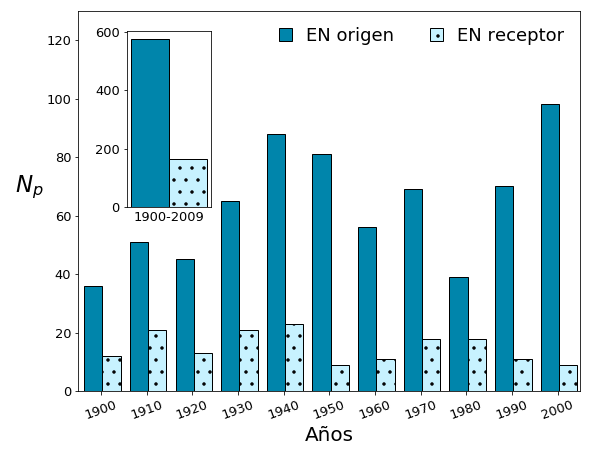
\includegraphics[width=0.5\textwidth]{BOR_EN.png} &
		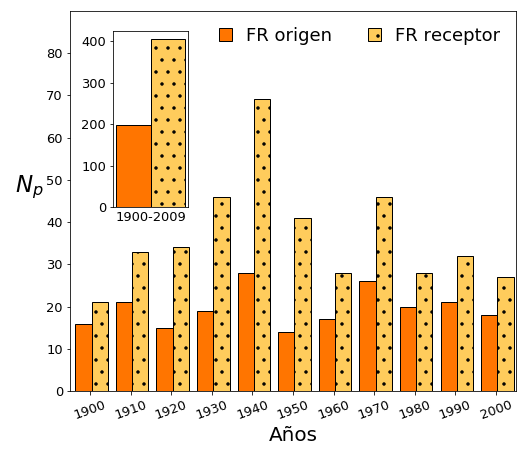
\includegraphics[width=0.5\textwidth]{BOR_FR.png} \\
		\textbf{(a)} & \textbf{(b)}   \\
	\end{tabular}

	\begin{tabular}{cc}
		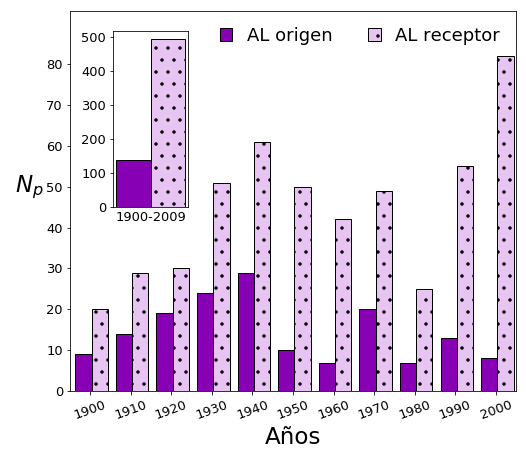
\includegraphics[width=.5\textwidth]{BOR_GE.png} &
		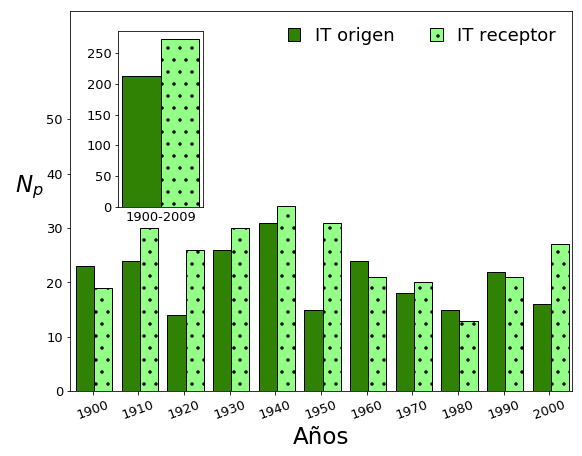
\includegraphics[width=.5\textwidth]{BOR_IT.png} \\
		\textbf{(c)}  & \textbf{(d)}   \\
	\end{tabular}
	\begin{tabular}{c}
		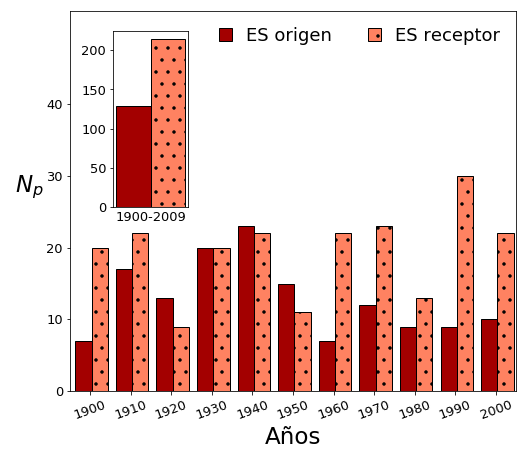
\includegraphics[width=.5\textwidth]{BOR_SP.png} \\
		\textbf{(e)} \\
	\end{tabular}
	\caption{Los idiomas como orígenes y receptores de palabras nuevas.
	Durante el siglo XX, sólo el inglés \textbf{(a)} ha sido el idioma que
	ha migrado más palabras de las que ha recibido. Francés \textbf{(b)},
	alemán \textbf{(c)}, italiano \textbf{(d)} y español \textbf{(e)}, han
	recibido más palabras durante la segunda mitad de siglo, tras finalizar
	la segunda guerra mundial. }
	\label{fig.RO_idiomas}
\end{figure} % }}}

La figura~\ref{fig.RO_idiomas} muestra el comportamiento de los idiomas al ser
orígenes o receptores de palabras nuevas.  El inglés ha aportado casi tres
veces más palabras de las que ha recibido, con sus mayores apogeos en 1940,
década que aconteció la segunda guerra mundial,  y en el 2000 tras la
globalización y el acceso a la tecnología en mayores sectores de la población. 

Francés y alemán, como receptores han sido similares, ambos recibiendo casi la
misma cantidad de palabras en cada década desde comienzos (1900) hasta mitad de
siglo (1950). Después de 1980, el alemán ha obtenido en cada década 30 palabras nuevas respecto a la década anterior, en consecuencia ha sido el mayor receptor en los últimos treinta años. Al tratarse como idioma origen, el alemán redujo la cantidad de palabras que aportaba en 1950, nuevamente tras finalizar la segunda guerra.

Referente al italiano, década a década, aporta casi la misma cantidad de
palabras que las que recibe, las únicas excepciones se dieron en 1920 y en
1950, tras finalizar la primera y segunda guerra mundial. 

Finalmente, el español en 1930 y en 1940, la cantidad de palabras que aporta y
que recibe es similar.  En las demás décadas, el español ha actuado primordial
mente como un idioma receptor. 

\subsection{Inglés} % {{{
\cpnote{aca vamos en el 3}

\begin{figure} [h!] % {{{
	\centering
	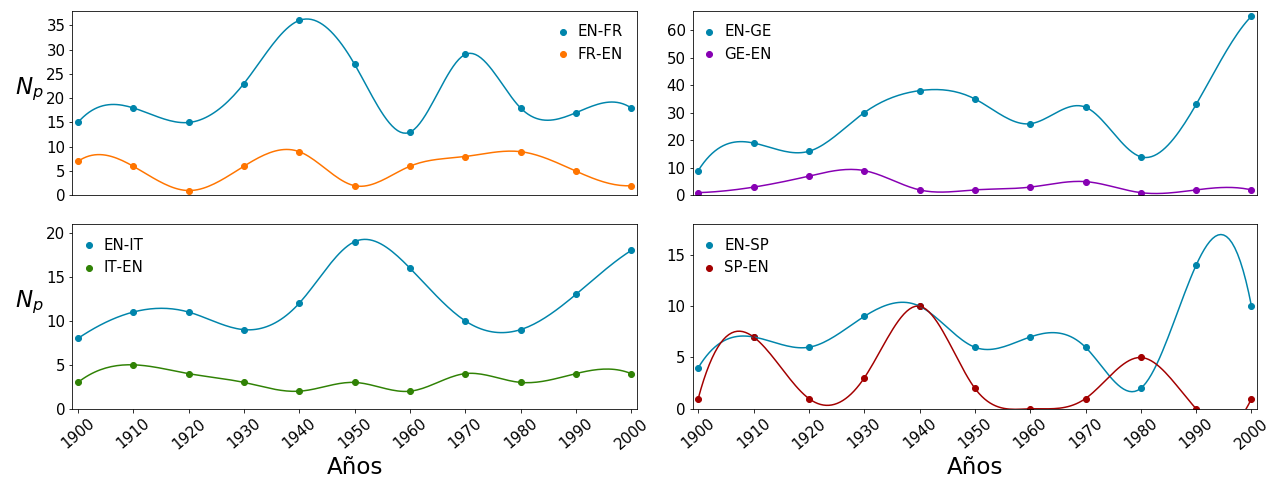
\includegraphics[scale=.33]{NC_EN.png}
	\caption{Palabras que migran del inglés a los demás idiomas y de los demás idiomas al inglés. El alemán ha sido el que más palabras recibe del inglés en promedio 29 cada década, seguido del francés con 21, el italiano con 12 y el español con 7. Los campos semánticos comunes en las migraciones del inglés a los demás idiomas son la política, la economía, la globalización y la tecnología.}
	\label{fig.NC_EN}
\end{figure} %  }}}

%De manera general, el idioma que más se ha beneficiado del inglés ha sido el alemán, con 300 préstamos en 100 años.  Inglés y alemán forman parte de las lenguas germánicas,  posible razón de los mayores intercambios. Entre las lenguas romances, el francés fue el más favorecido, pero también es la más similar por las relación normanda entre ambas.

De la figura~\ref{fig.NC_EN}, se puede ver que el inglés (con cualquier combinación) migró más palabras nuevas de las que recibió; las únicas excepciones se dieron  con el español en las décadas de 1910, 1040 y 1980. 
%A pesar de ser el mayor portador, la cantidad de palabras nuevas en los diferentes receptores no es homogénea, por ejemplo en el francés  la cantidad mínima por década es de 13, mientras que el español recibió un máximo de 14 en 1990.  Al tomarse como receptor hay más homogeneidad, ya que la media de palabras recibidas por década en cualquier combinación ronda  entre 3 y 5. 

Entre 1920 y 1950, el francés, el alemán y el italiano tuvieron un incremento de palabras del ingles. En este periodo las palabras encontradas son términos de las guerras, donde los Estados Unidos, el Reino Unido, Francia, Italia, Alemania y  el Imperio Austro-Húngaro estuvieron involucrados, a diferencia de España que no participo.   

Una tendencia similar se dio en los últimos veinte años (1980-2000), con un incremento del inglés en el alemán, el italiano y el español. El hecho con el que se relaciona el incremento es que el inglés se ha mostrado como un idioma común en la comunicación, la ciencia y la tecnología,  sumado al poder que obtuvo los Estados Unidos tras la segunda guerra mundial y donde su modelo económico prevaleció después de la guerra fría (conflicto que termino en 1990). 



\subsubsection*{Inglés-Francés} % {{{


Los mayores aportes se dieron entre 1930 y 1970, periodo que engloba comienzos de la Gran Depresión (1929), la Segunda Guerra Mundial (1939-1945) y la Guerra Fría (1945-1991), sucesos donde participaron países de ambas lenguas. Las palabras nuevas que refieren a estos eventos son \textit{churchill} (1944), \textit{territories} (1944), \textit{nazis} (1945), \textit{catastrophe} (1945), \textit{dollar} (1950), \textit{nixon} (1968) y \textit{johnson} (1970); las ultimas son apellidos de los presidentes de los Estados Unidos  Lyndon B. Johnson y Richard Nixon, cuyos periodos de gobierno fueron  entre 1963-1969 y 1969-1974 respectivamente.

% }}}
\subsubsection*{Inglés-Alemán} % {{{

Sólo  en dos décadas (1900  y 1980), el alemán no fue el idioma que más prestamos recibió  del ingles. Por el año de aparición, palabras como \textit{economic} (1929), \textit{depression} (1931), \textit{investment} (1933) y \textit{roosevelt} (1935), son del campo semántico de la economía y de la Gran Depresión,  mientras que  Franklin D. Roosevelt fue el presidente de los Estados Unidos que gobernó posterior a la crisis económica y durante la segunda guerra mundial. 

%La crisis económica de la gran depresión, originada en los Estados Unidos con consecuencias en diferentes países, entre ellos  Alemania, fue uno de los motivos que propició la segunda guerra mundial.

En las ultimas dos décadas, surgen términos referentes a la globalización y al desarrollo tecnológico, entre ellas \textit{standards} (1983), \textit{market} (1994), \textit{internet} (1996), \textit{economy} (1996), \textit{online} (1998), \textit{value} (2001), \textit{financial} (2003) y \textit{customer} (2007). 
% }}}
\subsubsection*{Inglés-Italiano} % {{{


Las palabras hacia el italiano, identificables en la primera mitad de siglo son \textit{roosevelt} (1941) y \textit{stalin} (1949), apellidos de personajes involucrados en la Segunda Guerra Mundial. En el caso de Joseph Stalin, a pesar de que su nacionalidad no es de algún país de habla inglesa, en el inglés su apellido tomó notoriedad para exportarse a los otros idiomas, siendo un ejemplo de palabras que se hacen populares en idiomas distintos al idioma origen. 

En los últimos años, nuevamente la globalización, la tecnología y la economía, son áreas comunes para los préstamos del inglés, \textit{internet} (1996), \textit{bussines} (2000) y \textit{marketing} (2001), son ejemplos de ellas. 


\subsubsection*{Inglés-Español} 

% aclarar esta justificacion
El español ha sido el idioma que menos préstamos toma del ingles,  sin  embargo es el idioma en el que migraron más apellidos de presidentes de los Estados Unidos, \textit{roosevelt} (1941), \textit{truman} (1950), \textit{kennedy} (1961), \textit{johnson} (1966),  \textit{nixon} (1972),  \textit{reagan} (1987), \textit{bush} (1990) y \textit{clinton} (1995).  Una de las posibles razones de encontrar en el español a estos personajes,  es por la relación y la mezcla cultural que han tenido los Estados Unidos con países de Latinoamérica.  

El los últimos años, las palabras aluden a términos de la globalización y la tecnología  \textit{internet} (1995), \textit{mail} (1999), \textit{marketing} (2001),  \textit{digital} (2002), \textit{software} (2004) y \textit{management} (2009).  

%A pesar de no ser el idioma más favorecido es al que en más areas ha impregnado el ingles, siendo este un factor que también puede indicar una mayor influencia,  en cuantas áreas esta presente un idioma y que tanto se utiliza. 

% }}}
% }}}
\subsection{Francés} % {{{

\begin{figure}[h!]
	\centering
	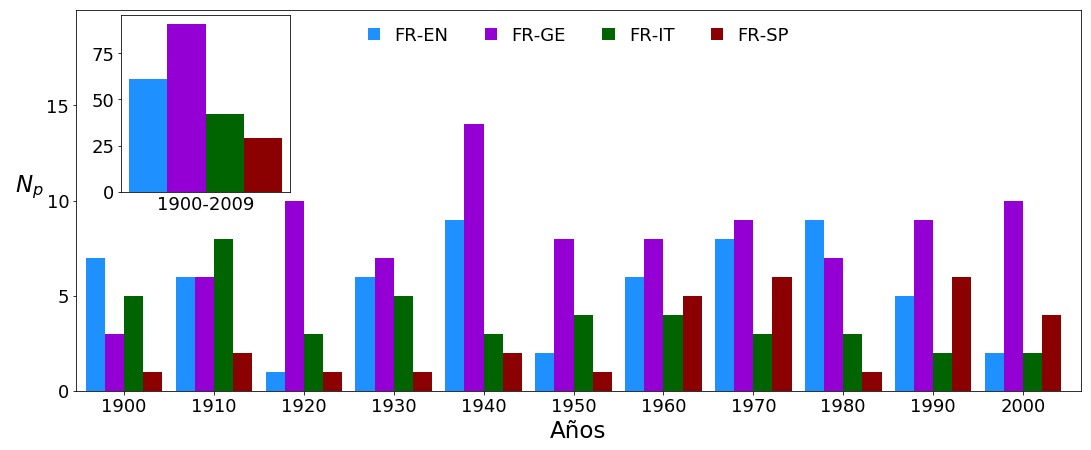
\includegraphics[scale=.33]{NC_FR.png}
	\caption{Palabras que migran del francés a los demás idiomas y de los demás idiomas al francés.  El inglés es el idioma que mas palabras recibe del francés, en promedio 8 por cada década, seguido del alemán con 5, el italiano con 3 y el español con 2. La primera y segunda guerra mundial son los campos semánticos más comunes en las migraciones del francés.}
	\label{fig.NC_FR}
	
	
\end{figure}

De la figura~\ref{fig.NC_FR} se puede ve que entre las décadas de 1920 y 1940,  incrementaron las palabras que migraron del francés en  el inglés, en el alemán y en el italiano. Las palabras que migran entre estas décadas son referentes a la Primera Guerra Mundial (que termino en 1918, año cercano a 1920) y a la Segunda Guerra Mundial (finalizada en la década de 1940). 

A pesar de que en los conflictos bélicos del siglo pasado no participaron países hispanohablantes, el español si recibió palabras que tomaron importancia tras la Segunda Guerra Mundial como lo son nombres de países y nombres de organizaciones. Este tipo de palabras son con las que se relaciona el incremento del francés en el español durante la segunda mitad de siglo. 



\subsubsection*{Francés-Inglés}% {{{

Durante el siglo XX, los préstamos en este sentido, se caracterizan por ser palabras comunes e identificables de origen inglés,  por ejemplo  \textit{diagnostic}, \textit{clients}, \textit{placement}, \textit{adaptation}, \textit{diffusion} y \textit{amplitude}.  A pesar de
que estas palabras pueden ser identificables como de origen inglés, las palabras si aparecieron primero en el francés dentro de las cinco mil palabras más usadas. 

Las palabras en este sentido son un ejemplo de las limitaciones que tiene el algoritmo para detectar el origen adecuado de las palabras. 

% }}}
\subsubsection*{Francés-Alemán}% {{{

El alemán tuvo dos décadas entre 1920 y 1940  (años cercanos a las dos guerras mundiales), donde  fue el idioma que más palabras recibió del francés. Entre estos años se localizaron a \textit{diplomatie} (1917), \textit{bourgeoisie} (1919), \textit{politique} (1920)  \textit{guerre} (1925), \textit{allemagne} (1925), \textit{russie} (1925) y \textit{empire} (1937), palabras del campo semántico de la política y de países involucrados en las guerras. 



% }}}
\subsubsection*{Francés-Italiano}% {{{

Las clasificaciones para esta pareja de origen y receptor son escasas, entre las pocas realizadas se encuentra un término del campo científico como \textit{poincare} (1924) (apellido del matemático francés Henri Poincaré);  y nombres de ciudades y países referentes a las dos guerras mundiales, \textit{austro} (1915), \textit{versailles} (1924), \textit{vietnam} (1966)  y \textit{urss} (1975).


% }}}
\subsubsection*{Francés-Español}% {{{


En el español, las palabras que provienen del francés son del campo semántico de la Posguerra de la Segunda Guerra Mundial. Entre ellas estan nombres de países como \textit{urss} (1962) y \textit{vietnam} (1965); y nombres de organizaciones \textit{onu} (1995) y  \textit{ocde} (2009). A pesar de que en la Organizacion de las Naciones Unidas (ONU) y en la Organización para la Cooperación y el Desarrollo Económico (OCDE) sean miembros países cuya lengua oficial no sea ni francés ni español,  en francés y español la abreviación de estas organizaciones es la misma.  

%




% }}}
% }}}
\subsection{Alemán}% {{{

\begin{figure}[h!]
	\centering
	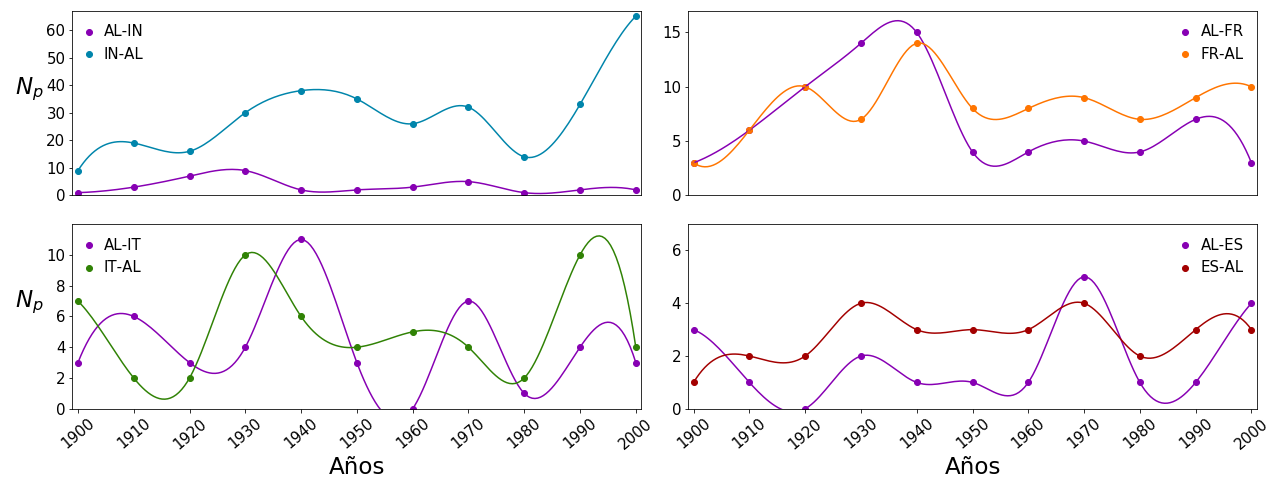
\includegraphics[scale=.33]{NC_GE.png}
	\caption{Palabras que migran del alemán a los demás idiomas y de los demás idiomas al alemán. El francés es el idioma que más palabras recibe del alemán,  en promedio 6 por cada década,  seguido del ingles y el italiano con 4,  por ultimo está el español con 2. Los campos semánticos más comunes en las migraciones del alemán son la guerra  y  los apellidos  de personajes germano parlantes que destacaron en algún área academia.}  
	\label{fig.NC_GE}
\end{figure}



De la figura~\ref{fig.NC_GE} se puede ver que entre las décadas de 1920 y 1940, en todos los idiomas aumentaron la cantidad de palabras que migraban del alemán. La participación de Alemania en los conflictos bélicos, propició las migraciones del campo semántico de la guerra en estas décadas. 

En la segunda mitad de siglo, las migraciones del alemán en los demás idiomas disminuyeron,salvo en la décadas de 1970 con el italiano y con el español, y en el 2000 con el español, resultando el alemán un idioma que recibió más palabras de las que migró. La derrota de Alemania en la Segunda Guerra Mundiales fue un factor para que el alemán en la segunda mitad de siglo recibiera más palabras de las que migró, adaptándose a ámbitos culturales, políticos y económicos de los demás países. 

Los personajes germano parlantes que destacaron en algún areá, con excepción de Hitler, no son identificables en la figura~\ref{fig.NC_GE}, ya que no migraron en el mismo año en que destacaron, y en cada receptor el año de migración es diferente. 


\subsubsection*{Alemán-Inglés}% {{{

En los años posteriores a la Segunda Guerra Mundial, se encontraron palabras ligadas al evento. Entre ellas \textit{lenin} (1931), \textit{hitler} (1934) y \textit{reich} (1939).  Otras palabras relevantes son \textit{beethoven} (1930), \textit{marx} (1934) y \textit{freud} (1934), apellidos de personajes destacados en la música, la filosofía y la psicología, todos ellos germano parlantes.


% }}}
\subsubsection*{Alemán-Francés}% {{{

%El francés ha recibido más palabras del alemán que cualquier otro. A pesar de que la mayor cantidad de aportes se dio en la primera mitad de siglo, las relaciones que se encontraron han sido a lo largo de todo el periodo y en diferentes áreas. 

Se distinguieron dos campos comunes para los préstamos nuevos,  el primero referente a la historia del alemán en las guerras, \textit{kaiser} (1915), \textit{reich} (1921), \textit{hitler} (1933),  \textit{regierung}, \textit{deutschen},\textit{minister} y  \textit{bestimmungen} todas ellas en 1944. % (traducciones de gobierno, alemán, ministro y reglamentos).  

El segundo campo, son apellidos de  personajes destacados en la filosofía \textit{nietzsche} (1905),  \textit{marx} (1923), \textit{engels} (1970) y \textit{heidegger} (1987); la psicologia \textit{freud} (1965)  y  la música \textit{mozart} (1956). 



\subsubsection*{Alemán-Italiano}% {{{

Los préstamos que migraron del alemán al italiano,  se encuentran palabras relacionadas con la guerra. Entre ellas \textit{reich} (1930),  \textit{hitler} (1939), \textit{lenin} (1944) y \textit{berchtold} (1944); mientras que 
\textit{nietzsche} (1903),  \textit{engels} (1948) y  \textit{heidegger} (1978) son de la filosofía; \textit{freud} (1970) en la psicologia; y \textit{mozart} (1942) y \textit{bach} (1949) en la música. 



%Nuevamente los préstamos del alemán,  son apellidos de personajes destacados en algun ar,  además de los ya mencionados, el único apellido exclusivo en el italiano fue \textit{berchtold} en 1943, referente a Leopold Berchtold, ministro de exteriores del Imperio Austro-Húngaro de 1912 a 1915, cuyo fallecimiento ocurrió en 1942. R


  
% }}}
\subsubsection*{Alemán-Español}% {{{

A pesar de que el español no estuvo involucrado en la segunda guerra mundial, si migrarón a él terminos relacionados con el suceso.  Entre ellos \textit{kaiser} (1938) y \textit{hitler} (1940). 

Las demás palabras son nuevamente  apellidos de personajes, \textit{marx} (1932), \textit{lenin} (1970), \textit{hegel} (1971),  \textit{nietzsche} (2000) y \textit{freud} (2002). Estas palabras a pesar de ser comunes en las migraciones del alemán, la migración hacia el español ocurrió después que los demás idiomas, por ejemplo en el francés Nietzsche apareció en 1905 y Freud en 1934. La diferencia en los años de migración puede ser un indicio de la adaptabilidad de una lengua en otra, aunque en este trabajo no se ha desarrollado esta idea. 



% }}}
% }}}

% {{{

\clearpage
\subsection{Italiano}
 
 
\begin{figure}[h!]
	\centering
	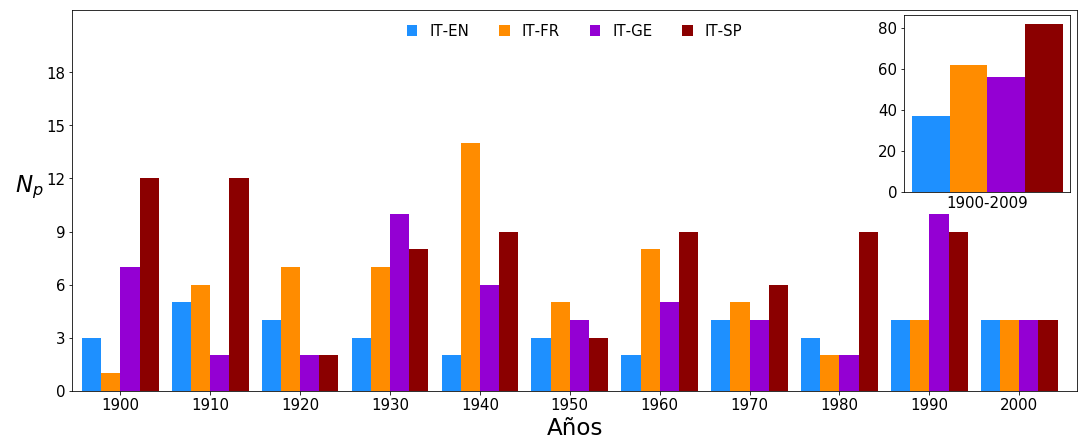
\includegraphics[scale=.33]{NC_IT.png}
	\caption{Palabras que migran del italiano a los demás idiomas y de los demás idiomas al italiano.  El español es el idioma que más palabras recibe del italiano, en promedio 8 por cada década, seguido del francés con 6,  el alemán con 4 y el inglés con 3. Los campos semánticos de la guerra y la política comunes en la migraciones del italiano .} 
	\label{fig.NC_IT}
\end{figure}



De la figura~\ref{fig.NC_IT} se observa que unicamente con el ingles, el italiano ha sido exclusivamente un idioma receptor,  con los demás idiomas,  el italiano es tanto el que más palabras migra como el que más recibe. 

Las migraciones del italiano en el alemán, en el francés y en español, aumentaron  entre 1920 y 1940,  coincidiendo este periodo con las dos guerras mundiales (La Primera Guerra mundial termino en 1918, año cercano a 1920), situaciones donde participo Italia, por lo que los préstamos son referentes a estos  sucesos. 

En todos los idiomas,  a partir de 1990, se presenta un descenso en la cantidad de palabras que llegan del italiano, posiblemente al no estar relacionado el italiano con la globalización y el desarrollo tecnológico, los sucesos más importantes  desde esa década.   

\subsubsection*{Italiano-Inglés}% {{{

A pesar de que en cada década existen términos nuevos en el inglés, sólo fue posible relacionar \textit{mussolini} (1935),  alusivo al político y militar Benito Mussolini,  posiblemente el personaje italiano más relevante en la historia del siglo XX .

% }}}
\subsubsection*{Italiano-Francés}% {{{



En las migraciones sólo se asoció \textit{mussolini} (1935), la cual ya se había mencionado. Aunque en 1940 migraron la mayor cantidad de préstamos, ninguno se logro relacionar con eventos al rededor de la década. 

Tras revisar las listas de los préstamos nuevos con origen italiano  en los demás idiomas, Mussolini se encuentra en todas ellas, donde el año de migración es siempre 1935.





% }}}
\subsubsection*{Italiano-Alemán}% {{{

En este sentido de migración,  existen relaciones con el contexto bélico,  \textit{regime} (1938), \textit{panzer} (1941), \textit{duce} (1942),  traducciones de régimen, blindado y líder.

%además de \textit{Mussolini} (1935). 



% }}}
\subsubsection*{Italiano-Español}% {{{

En el español, además de los términos de la guerra, se encontraron nombres de términos políticos y sociales que tuvieron un auge en el siglo pasado. Palabras como  \textit{socialista} (1914), \textit{comunista} (1932), \textit{capitalismo} (1935), \textit{fascismo} (1937),  \textit{marxismo} (1963) y \textit{terrorismo} (1986) son ejemplo de ellos. 

% }}}
% }}}


\subsection{Español}% {{{

\begin{figure}[h!] % {{{
	\centering
	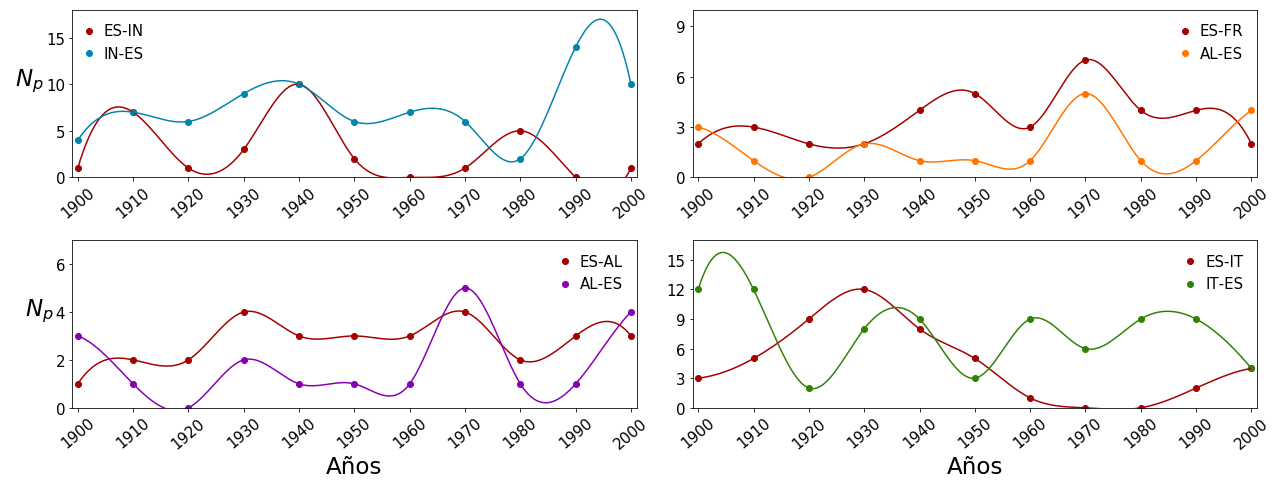
\includegraphics[scale=.33]{NC_SP.png}
	\caption{Palabras que migran del español a los demás idiomas y de los demás idiomas al español. El italiano es el idioma que más palabras recibe del español, en promedio 5 por cada década, seguido del francés con 3, mientras que el ingles y el alemán reciben 2. Los campos semánticos donde provienen los préstamos del español  más comunes en las migraciones del español son la medicina y los nombres de países y Latinoamericanos. }
	\label{fig.NC_SP}
\end{figure} % }}}


De la figura~\ref{fig.NC_SP}, se pueden ver comportamientos similares en las migraciones del español en los demás idiomas, con incrementos en la primera década del siglo y entre las décadas de 1930 y 1940,  y una disminución desde 1990. En algunos casos las migraciones fueron nulas, en el ingles en las décadas de 1960 y 1990, mientras que en el italiano fueron entre las décadas de 1970  y 1980. 

Tras revisar los pŕestamos del español en los diferentes receptores,  la característica común de los préstamos es que son términos médicos, migrando en los diferentes receptores en la primera mitad de siglo, por lo que son la principal razón de del incremento entre 1930 y 1940. 

Al igual que en el italiano, las migraciones del español en los demás idiomas (salvo en el italiano) decayeron a partir de la década de 1990, ya que el español no ha tenido relación con la globalización y el desarrollo tecnológico. 

\subsubsection*{Español-Inglés}% {{{

Contrario a la tendencia en las migraciones anteriores, la guerra no es un campo semántico común en el contenido de los préstamos. La mayor parte de los términos son habituales en la medicina,  en 1943  aparecieron  \textit{virus} y \textit{anemia};  años antes en 1934 George Richards Minot, Parry Murphy y George Hoiyt Whipple, habían recibido el premio Nobel de medicina por su descubrimiento de la terapia de hígado para el tratamiento de anemias.   

Otras palabras importantes son nombres de países hispanohablantes \textit{chile} (1919) y \textit{argentina} (1940); de acuerdo a \cite{crisis_chile} tras la primera guerra mundial, Chile se vio en una crisis económica  que culmino hasta 1930 gracias al desarrollo de la industria fabril chilena; por otra parte a la década de 1930 también se le conoce como la década infame en la historia argentina, debido a la crisis económica que sufrió el país  y que llevo a un golpe de estado durante el mandato del presidente Hipólito Yrigoyen. 

\subsubsection*{Español-Francés}% {{{

El primer préstamo con contenido es \textit{panama} (1913), su importancia se debe a la inauguración del canal de Panamá en 1914. Destaca que la palabra llegue al francés por ser el gobierno de Francia el que impulsó económicamente su construcción, aunque su conclusión y administración pasó a los Estados Unidos.  




% }}}
\subsubsection*{Español-Alemán}


Los préstamos son nuevamente términos médicos, además \textit{virus} y \textit{anemia} mencionados en las migraciones hacia el inglés. Como termino exclusivo en el alemán  se encontró a \textit{lepra} (1901), debido a que en 1874, Gerhard Armauer Hansen descubrió el bacilo de Leprae que origina la enfermedad.

%fue globalmente importante a partir de 1874,  ya que en ese año el científico noruego Gerhard Armauer Hansen descubrió el bacilo de Hansen Mycobacterium Leprae \cite{lepra} que origina la enfermedad. Por el carácter médico de la palabra, es probable que se hiciera más investigación sobre la enfermedad en diferentes idiomas, en este caso el alemán. 


% }}}
\subsubsection*{Español-Italiano}% {{{

Además de los términos médicos ya mencionados, en el italiano migraron de forma  exclusiva  \textit{virus} (1922), \textit{colesterina} (1928),  \textit{sintomatología} (1931), \textit{anestesia} (1932), \textit{vitamina} (1935), \textit{anemia} (1936), \textit{metabolismo} (1936),  \textit{gástrica} (1936)  y \textit{endovenosa} (1937).  

También destacan las palabras  \textit{buenos} (1900) y \textit{aires} (1901), referentes a Buenos Aires, la capital de Argentina . Este préstamo esta ligado a la migración de personas,  ya que desde 1862 hasta 1970, incremento la población de italianos en Argentina,  asentándose principalmente en la ciudad de Buenos Aires,  además para 1900 los inmigrantes italianos representaban casi 20$\%$ de la población en Argentina.  Tras la inmigración de italianos en Argentina, es común pensar que esta mezcla origino cambios culturales, entre ellos en los idiomas. 

%El aparecer estas palabras en el español (dentro de las cinco mil más usadas)antes que en los demás,  sugiere que la medicina era un campo importante para los países de habla española, donde posiblemente se publicaron más libros de medicina en esta lengua. 






% }}}
% }}}
% }}}
\section{Resultados generales}% {{{



Tras las múltiples combinaciones entre idiomas, la relación habitual son palabras del campo semántico de la guerra, la mayor parte de ellas, surgieron en los diferentes receptores durante y después de la Segunda Guerra Mundial. 

En cada idioma, las migraciones de palabras son recurrentes de ciertos campos semánticos,  el inglés en economía, tecnología y política; el español en medicina, y en la cultura de los países Latinoamericanos; el francés y el italiano en la guerra; mientras que en el alemán además de la guerra también son comunes las áreas académicas  a partir de personajes germano parlantes que destacaron en ellas. .  

Las áreas mencionadas, no brindan una respuesta sobre que idioma ha sido más influyente, pero si en cuales campos un idioma ha influido más que los otros, siendo esta una forma alternativa de hablar de influencia en los idiomas.
 
Una manera diferente de estudiar a los préstamos nuevos, sería a través del tiempo que le toma a las palabras moverse de un idioma a otro, con ello, se pueden obtener la velocidad con la que migran y su adaptabilidad en las diferentes lenguas receptoras. Aunque estos resultados pueden ser complementarios, por el momento no se han tratado. 


%El inglés se presenta en las últimas dos décadas como el idioma común para transmitir información, exportando términos comunes en ámbitos como  la globalización y el desarrollo  de la tecnología.  Destaca el rol de los Estados Unidos como un país involucrado en los principales acontecimientos que originaron las migraciones, siendo usuales los apellidos de todos sus presidentes (posteriores a la segunda guerra mundial) en los demás idiomas. 

%Salvo el inglés que fue exportador en distintas áreas, los demás idiomas se caracterizaron por brindar palabras especificas,  el alemán por apellidos de personajes, el español por términos médicos, mientras que el francés y el italiano por la historia bélica y la religión. . 

 %Estos posibles resultados ayudarían a complementar la relación entre eventos, ya que en algunos eventos las palabras asociadas a él, migraron a los demás idiomas  en el mismo periodo, por ejemplo,  las palabras que migraron tras la revolución francesa (1789-1799) aparecieron en los diferentes receptores mientras ocurría el suceso y hasta veinte años después de él; así mismo,  los términos involucrados en la globalización  posterior a 1980 migraron en los años inmediatos a su invención.  Para tales complementos se necesitaría separar a los préstamos por áreas, lo cual no se hizo en este trabajo.  












% }}}





%\include{Capitulo2/marco_teorico}           % ~20 páginas - Poner un contexto a la tesis, hacer referencia a trabajos actuales en el tema
\chapter{Palabras acumuladas}

La búsqueda para cuantificar la influencia, ha llevado a contabilizar las palabras que son nuevas en los distintos receptores y a partir de ellas ligar contextos que sustenten la aparición de palabras.  Se ha puesto énfasis en el conjunto de búsqueda, pero  el conjunto base  también tiene información sobre las palabras que han migrado, además  abarca más años (160 comprendidos entre 1740 y 1900), por lo que su información es más basta en contenido. 

Para no repetir el proceso de contabilizar a los préstamos nuevos,  se propone pensar que en el primer año del conjunto de búsqueda (1900),  el idioma receptor ya contenía cierta cantidad de palabras que provenían de otros orígenes,  de tal manera que ya forman parte de él, es decir estos préstamos ``conviven'' con las palabras propias de el receptor y son empleadas indistintamente. Así el conjunto base proporcionará un sostén de aquellas palabras que han permeado en un idioma y son utilizadas en los años del conjunto de búsqueda,  cabe decir que este sostén crecerá conforme se localicen nuevas palabras. 

Es necesario hacer una nueva definición para estos préstamos, dados un idioma  origen  \textit{A} y la lista para un año  de las palabras más comunes en el receptor \textit{B}, se definen como: 

\begin{description}
	\item[préstamos acumulados:] Son las palabras con origen \textit{A} que ya habían aparecido en alguna lista de \textit{B}, y para ese año lo volvieron a hacer.  
\end{description}

La diferencia entre los nuevos y los acumulados es que un préstamo será nuevo sólo en el año de aparición, posteriormente se convertirá en acumulado. El objetivo  de trabajar con los acumulados es ver cómo se comportan las palabras que ya han migrado a un receptor y si hay tendencias donde su empleo se vea alterado.  

En el capitulo anterior, la atención se enfocaba en la cantidad de palabras, nunca se trato con su frecuencia o su rango, ahora se utilizarán estas propiedades  para llegar a una cantidad que cuantifique la influencia. Si se tienen la lista de las cinco mil palabras más usadas  de \textit{B}, y se distinguen en ella los préstamos acumulados con origen \textit{A}, entonces: 

\newpage

\begin{enumerate}
	
	\item En un año determinado del idioma \textit{B}, se sumarán las frecuencias $f_{k}$ de las cinco mil palabras más usadas.  Esta cantidad se llamará \textbf{frecuencia total} $f_{t}$ y es distinta año con año. 
	
	\begin{equation}
	\label{ec.ftot}
	f_{t} = \sum_{k=1}^{5000} f_{k} \,\,\,\,\,\,\,\,\, k = rango\,\, de \,\,cada \,\,palabra
	\end{equation}
	
	\item Como se conocen los rangos $j$,  que ocupan los préstamos \textit{A} en la lista de \textit{B}, se procede a sumar sólo las frecuencias asociadas a estas palabras. Esta cantidad será la \textbf{frecuencia de préstamo} $f_{p}$,  siempre será menor que la frecuencia total.
	
	\begin{equation}
	\label{ec.fpres}
	f_{p} = \sum_{j} f_{j} \,\,\,\,\,\,\,\,\, j = rango\,\, de \,\,cada \,\,pr\acute{e}stamo\,\,acumulado
	\end{equation}
	
	
	\item  Se divide la frecuencia de préstamo entre la frecuencia total , esta cantidad se llamará  \textbf{Uso} $U$ y es la porción que representa \textit{A} en \textit{B} en teŕminos de frecuencia.  Como en un año hay más palabras propias de B, esta cantidad es muy pequeña, para tener cifras manejables, se tomara un porcentaje al multiplicar el cociente por cien.  

	\begin{equation}
	\label{ec.fuso}
	 U = \frac{f_{p}}{f_{t}} * 100
	\end{equation}
	
	
	Entre más cercana a 100$\%$ sea el \textit{Uso de A en B}, los préstamos de \textit{A} son más relevantes en \textit{B}.

\end{enumerate}

Lo relevante de trabajar con esta cantidad es que en una lista de un determinado receptor existen préstamos acumulados con distintos orígenes, cada uno tendrá un valor diferente de uso, con ellos se puede inferir el origen que ha sido más relevante para el receptor. 


\newpage

\section{La influencia en 109 años}

Descritas el tipo de palabras a emplear y la forma de trabajar con ellas, el proceso que se siguió para obtener resultados es el siguiente: 

\begin{itemize}
	
	\item Elegidos un  origen \textit{A} y un receptor \textit{B}, se localizaron los prestamos acumulados de \textit{A} en \textit{B}.
	
	\item Se empleó la ecuación \ref{ec.fuso} en todos los años del conjunto de búsqueda, obteniendo 109 valores. 
	
	\item El proceso se repitió para todas las combinaciones de orígenes y receptores.
	
	\item  Tras cada año del conjunto de búsqueda y por cada pareja de origen y receptor, se elaboraron  listas con los préstamos acumulados, ordenándolos de forma descendente a partir de su frecuencia. 
	
	\item Para observar los datos como una cantidad que varia en el tiempo, se  hicieron tres tipos de graficas con tres tipos de agrupaciones.
	
	\begin{description}
		
		\item[\textit{A} como origen común.] Graficando el uso de \textit{A} en todos los demás.
		
		\item[\textit{A} como receptor común.] Graficando el uso de los demás en \textit{A}.
		
		\item[Alternando \textit{A} y \textit{B}.]  Graficando de manera conjunta el uso de \textit{A} en \textit{B}, y el de \textit{B} en \textit{A}.
				
	\end{description}	

\end{itemize}

Las listas elaboradas se emplearán en los siguientes capítulos, en el apéndice 1 se explica la forma de leerlas así como un vinculo para su consulta. 

\subsection*{Presentación de resultados}

Por cada idioma se presentarán dos graficas, la primera será tomando al idioma como origen y la segunda al tomarlo como receptor. Se seguirá utilizando la nomenclatura descrita en el capítulo anterior sobre las abreviaciones y los colores.  Además se provee información de los campos semánticos comunes que hacen posible la prevalencia de los préstamos. 

En el apéndice A se agregarán las graficas de uso entre dos idiomas, estas servirán para complementar los resultados expuestos en esta sección.


Adicionalmente, la tabla \ref{tab.cantidad_acumulados} muestra la cantidad promedio de préstamos acumulados encontrados en cada año del conjunto de búsqueda. La idea de la tabla y el método del uso, es observar que el idioma que más palabras aporta a un receptor no es siempre el más utilizado,  el uso es mayor si las préstamos tienen rangos mas bajos (frecuencias altas). 


\begin{table}
	\centering
	\begin{tabular}{lcccccc}
		\multicolumn{7}{c}{R E C E P T O R}                                                                                                                                             \\
		\multirow{6}{*}{\begin{tabular}[c]{@{}l@{}}O\\ R\\ \,I\\ G\\ E\\ N\end{tabular}} &             & \textbf{EN} & \textbf{FR} & \textbf{GE} & \textbf{IT} & \textbf{SP} \\
		& \textbf{EN} & -           & 324.43      & 164.33      & 77.5        & 73.61       \\
		& \textbf{FR} & 297.36      & -           & 94.06       & 118.55      & 66.31       \\
		& \textbf{GE} & 63.87       & 48.06       & -           & 34.92       & 16.61       \\
		& \textbf{IT} & 77.82       & 100.62      & 47.9        & -           & 219.45      \\
		& \textbf{SP} & 118.43      & 84.22       & 29.85       & 311.97      & -          
	\end{tabular}
	\caption{Promedio de préstamos acumulados entre idiomas. Se aprecian dos relaciones reciprocas entre el inglés con el francés y el español con el italiano, donde no importa cual actué como receptor, el otro idioma es el origen del que provienen la mayor cantidad de palabras.}
	\label{tab.cantidad_acumulados}
\end{table}




\clearpage
\subsection{Inglés}


\begin{figure}[h!]
	\centering
	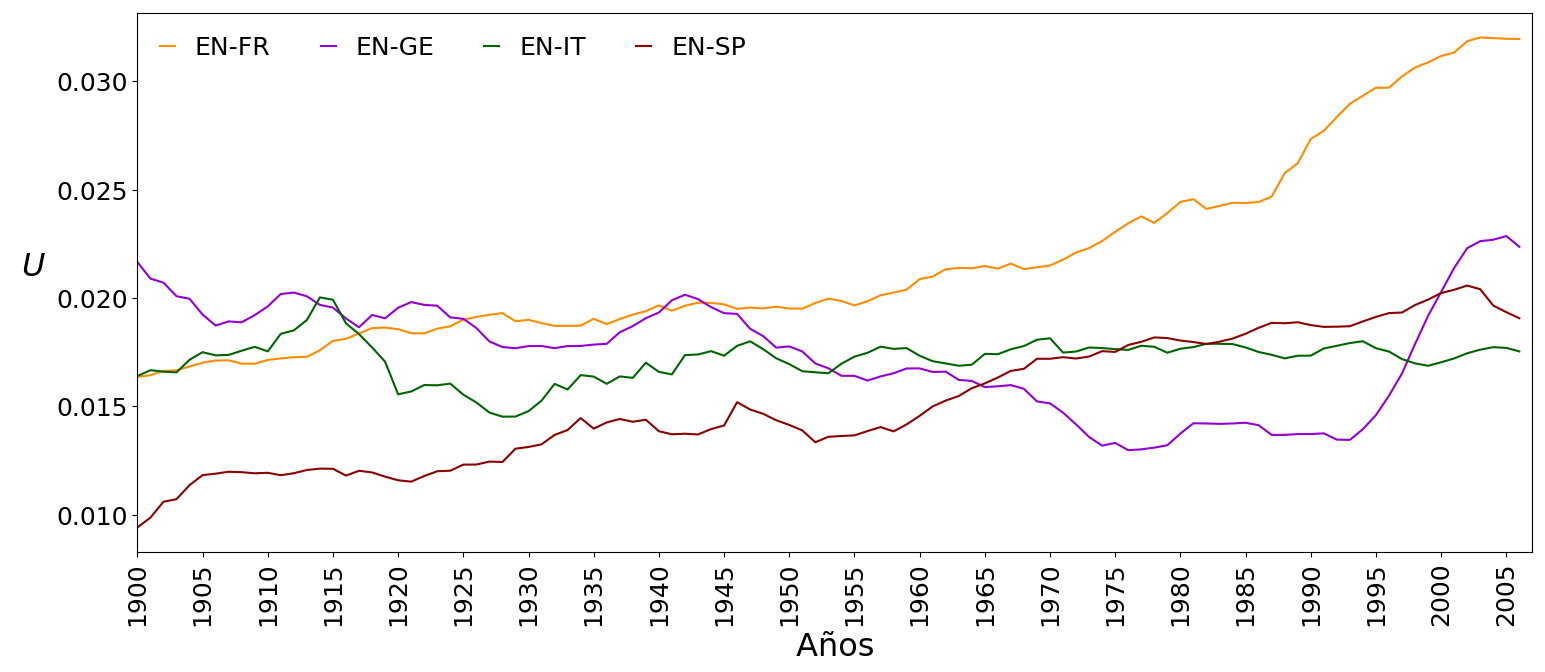
\includegraphics[scale=.36]{PF1_S2_EN.png}
	\label{fig.ST_a_EN}
	\caption{El inglés en los demás. El francés es el idioma donde más se ha empleado inglés, sin embargo en el español ha sido el de mayor crecimiento comparado en su uso en principios y en final de siglo.}
\end{figure} 



\begin{figure}[h!]
	\centering
	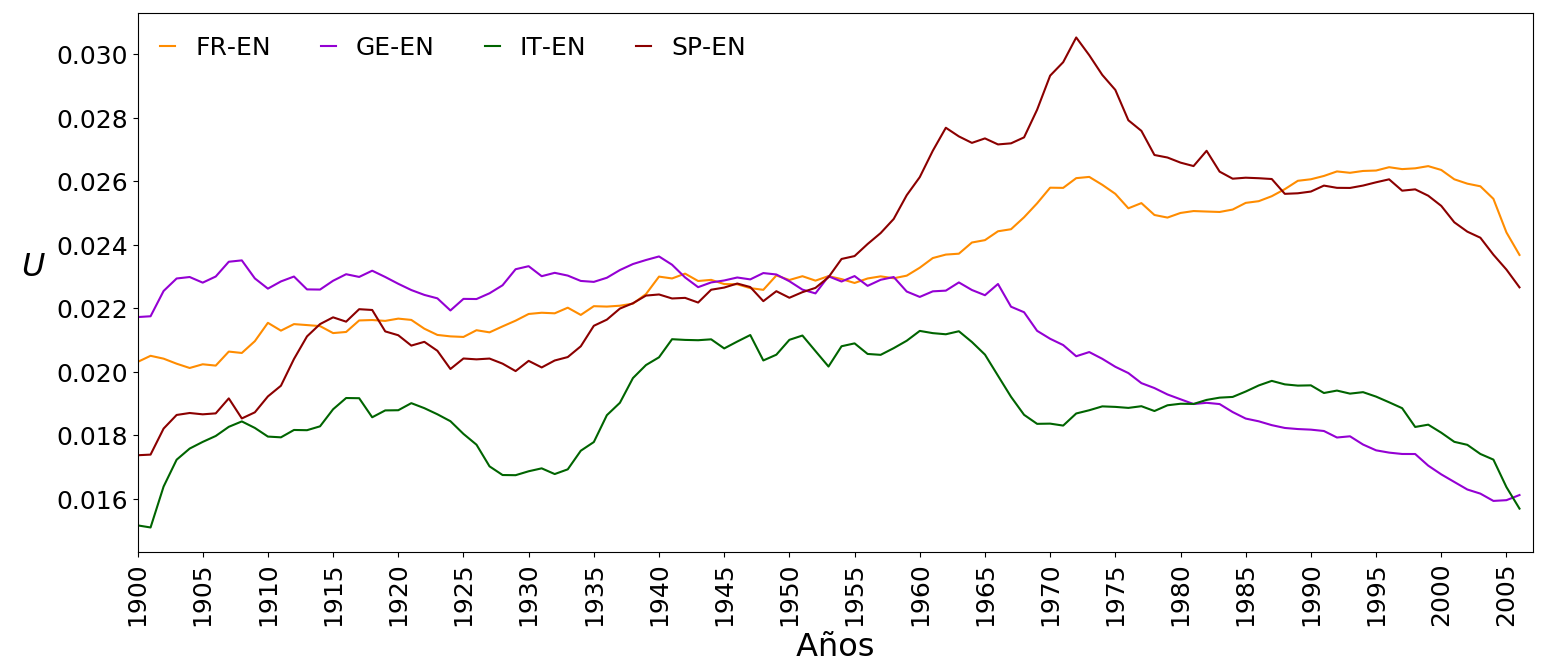
\includegraphics[scale=.36]{PF2_S2_EN.png}
	\label{fig.ST_b_EN}
	\caption{Los demás en el inglés. En los últimos 50 años, el español ha sido el idioma que es más utilizado en el ingles, seguido del francés, debido a las relaciones comerciales entre países de ambas lenguas.  Tras la segunda guerra mundial, alemán e italiano decayeron consistente en ser lengua de los países vencidos. }
\end{figure} 


\clearpage

El uso del ingles en los demás ha visto un continuo incremento posterior a 1945 en francés, en italiano y en español, mientras que en  alemán se da posterior a 1990, año donde culmina la guerra fría y se da la finalización del socialismo en Europa con la re-unificación de Alemania. El significado común de los   préstamos acumulados que aparecen en los cuatro conjuntos y que con los años descienden en rango son términos económicos y referentes a la industria como  \textit{capital}, \textit{dollar}, \textit{invesment}, \textit{relations}, \textit{market}, \textit{company}, \textit{development}, \textit{financial},  \textit{institutions}, \textit{internet} y \textit{software}. Otra característica relevante es la aparición continua de los apellidos de los presidentes de los Estados Unidos (posteriores a la guerra) durante el periodo en el cual gobernaron.  Apoyado de la información de los préstamos nuevos, se puede confirmar que el inglés se ha beneficiado del crecimiento de los Estados Unidos para ser exportado a las demás lenguas y ser el idioma común para transmitir información.   


En los últimos cincuenta años, los idiomas mas comunes en el ingles han sido el español y el francés,  nombres de países latinoamericanos como \textit{México}, \textit{Cuba}, \textit{Chile}, \textit{Nicaragua} y \textit{Argentina}, caracterizan a los acumulados del español, mientras que en el francés en su mayoría son palabras que bien podrian catalogarse de origen inglés, entre ellas \textit{royals}, \textit{religion}, \textit{saint}, \textit{passage} o \textit{court}. Tras brevemente ver ambos conjuntos se infiere que el español ha logrado instaurarse en el inglés por la relevancia de estos países en las relaciones o conflictos que tuvieron en el siglo pasado y donde intervinieron países de habla inglesa, contrario  al francés que prevalece por las relaciones culturales y etimológicas que existen entre ambas lenguas.

Por parte de las palabras con origen alemán e italiano no se logró relacionarlas a un campo semántico común. 


\clearpage
\subsection{Francés}

\begin{figure}[h!]
	\centering
	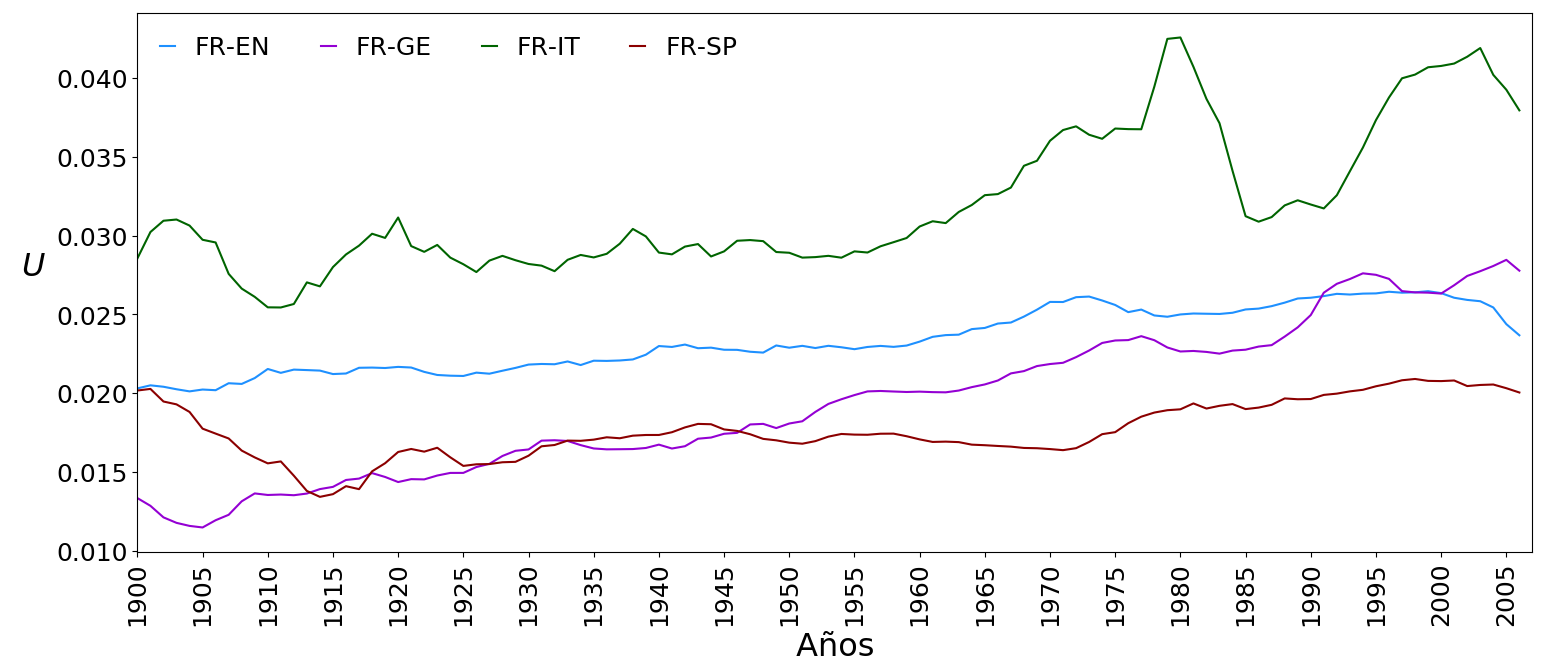
\includegraphics[scale=.36]{PF1_S2_FR.png}
	\label{fig.ST_a_FR}
	\caption{El francés en los demás idiomas. El italiano empleó más al francés durante todo el siglo XX, caracterizado por palabras comunes en la industria vitivinícola.}
\end{figure}


\begin{figure}[h!]
	\centering
	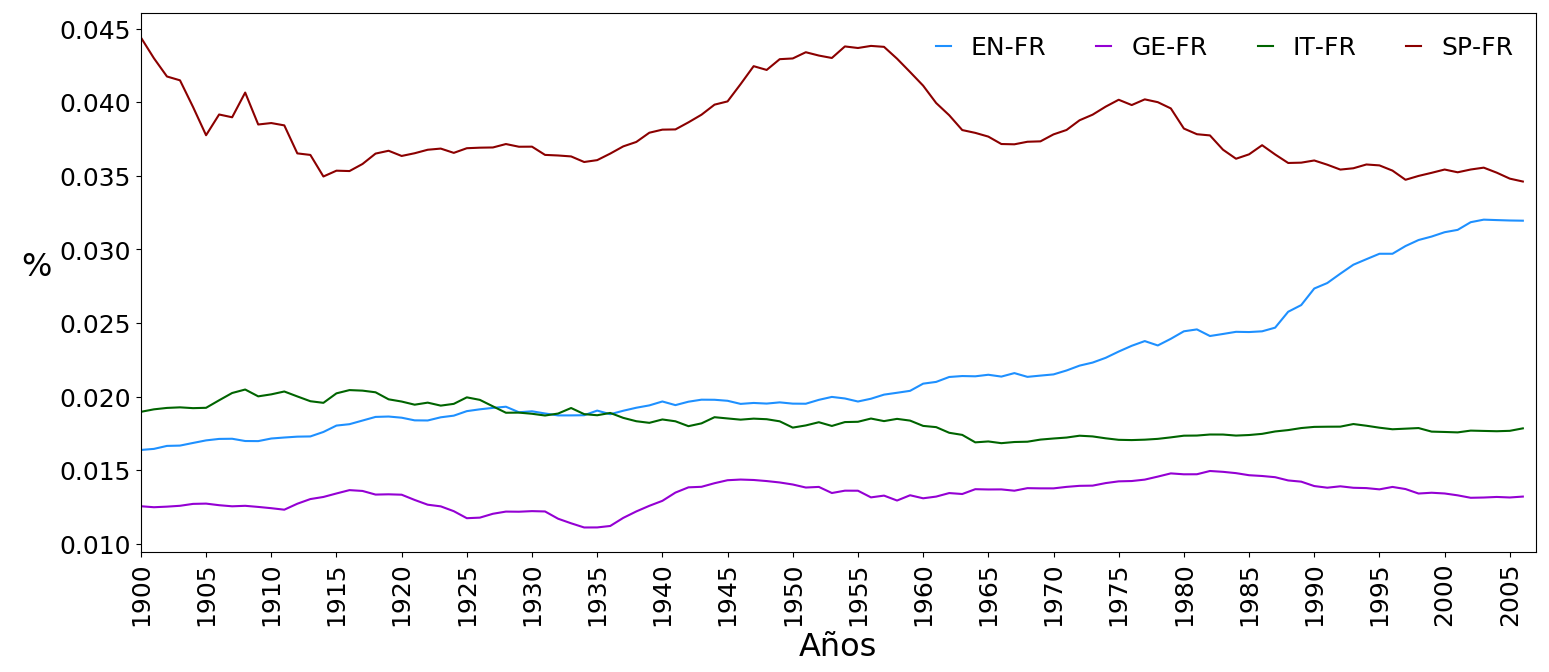
\includegraphics[scale=.36]{PF2_S2_FR.png}
	\label{fig.ST_b_FR}
	\caption{Los demás en el francés. El español ha resultado el de mayor presencia en el francés, en su mayoria son palabras con etimologías grecolatinas, comunes para ambas lenguas al provenir de la misma familia lingüística.}
\end{figure}
		
\clearpage


A pesar de que el idioma que más préstamos toma del francés es el inglés,  el idioma que más utiliza el francés ha sido el italiano,  aspecto que se mantuvo durante todo el siglo del análisis,  la industria vitivinícola, surgen como un conectores entre ambas lenguas al estar presente términos como  \textit{raisins}, \textit{vin}, \textit{vignoble} y \textit{recolte},  siendo una actividad común entre Francia e Italia.  Los préstamos hacia los demás idiomas son de carácter religioso o politico, destacando que tuvo el francés en estos ámbitos, a pesar de que la búsqueda se centre en el siglo XX, las mayores migraciones del francés surgen a partir de 1800, posteriores a la revolución francesa; entre las palabras que se han mantenido desde este acontecimiento están  \textit{saint}, \textit{eglise}, \textit{dime}, \textit{reine}, \textit{guerre}, \textit{imperiale}, \textit{royals} o \textit{bourgeois}.  


Para los prestamos usados en el francés el español y el inglés se muestran como los idiomas con mayor presencia, la característica común de los vocablos de ambos idiomas es que son palabras con etimología grecolatina, 
\textit{depression}, \textit{canal}, \textit{proceso}, \textit{services}, \textit{justice} entre otras,  siendo razonable la aparición de estas palabras por tener las tres lenguas una composición grecolatina. 


\clearpage
\subsection{Alemán}

\begin{figure}[h!]
	\centering
	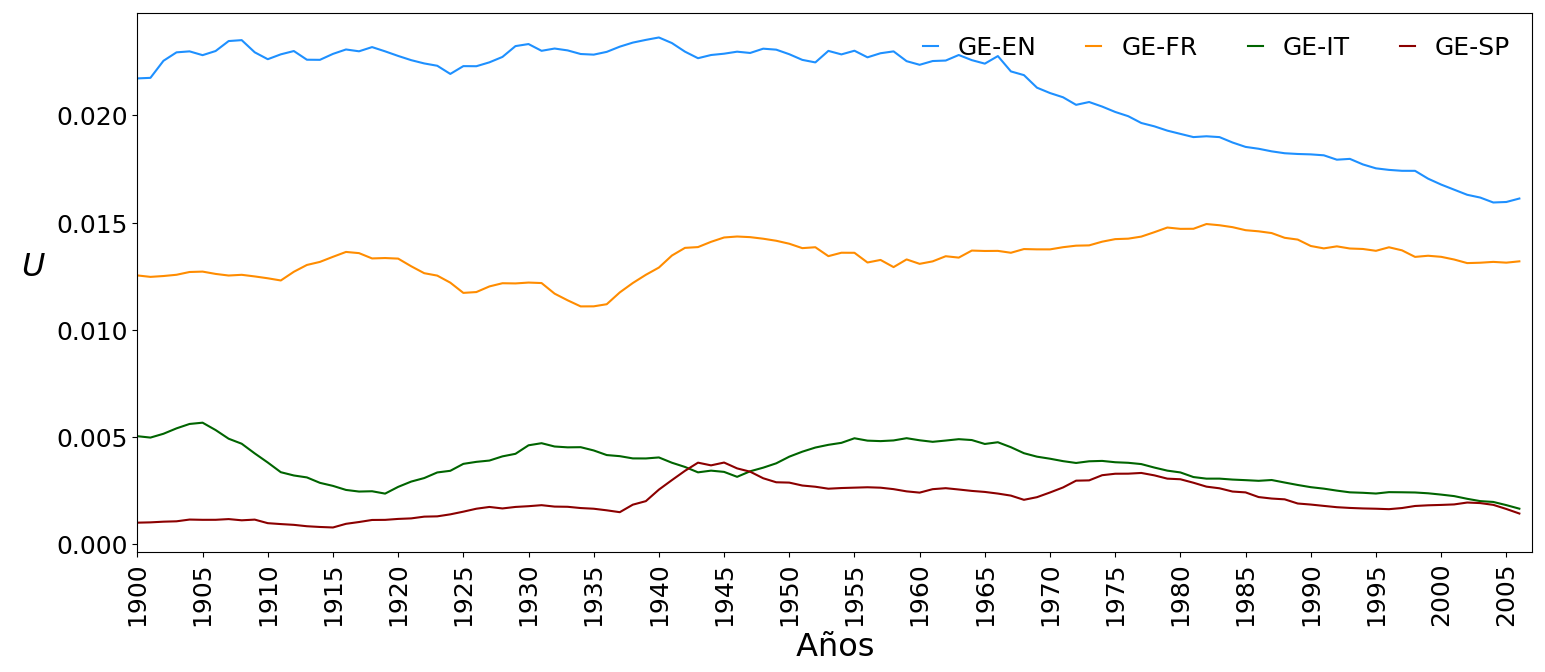
\includegraphics[scale=.36]{PF1_S2_GE.png}
	\label{fig.ST_a_GE}
	\caption{El alemán en los demás. La familiaridad por provenir de la misma rama lingüística hace posible que el inglés sea el idioma  donde los préstamos del alemán sean continuamente utilizados, siendo evidente la diferencia con las lenguas romances.}

\end{figure}


\begin{figure}[h!]
	\centering
	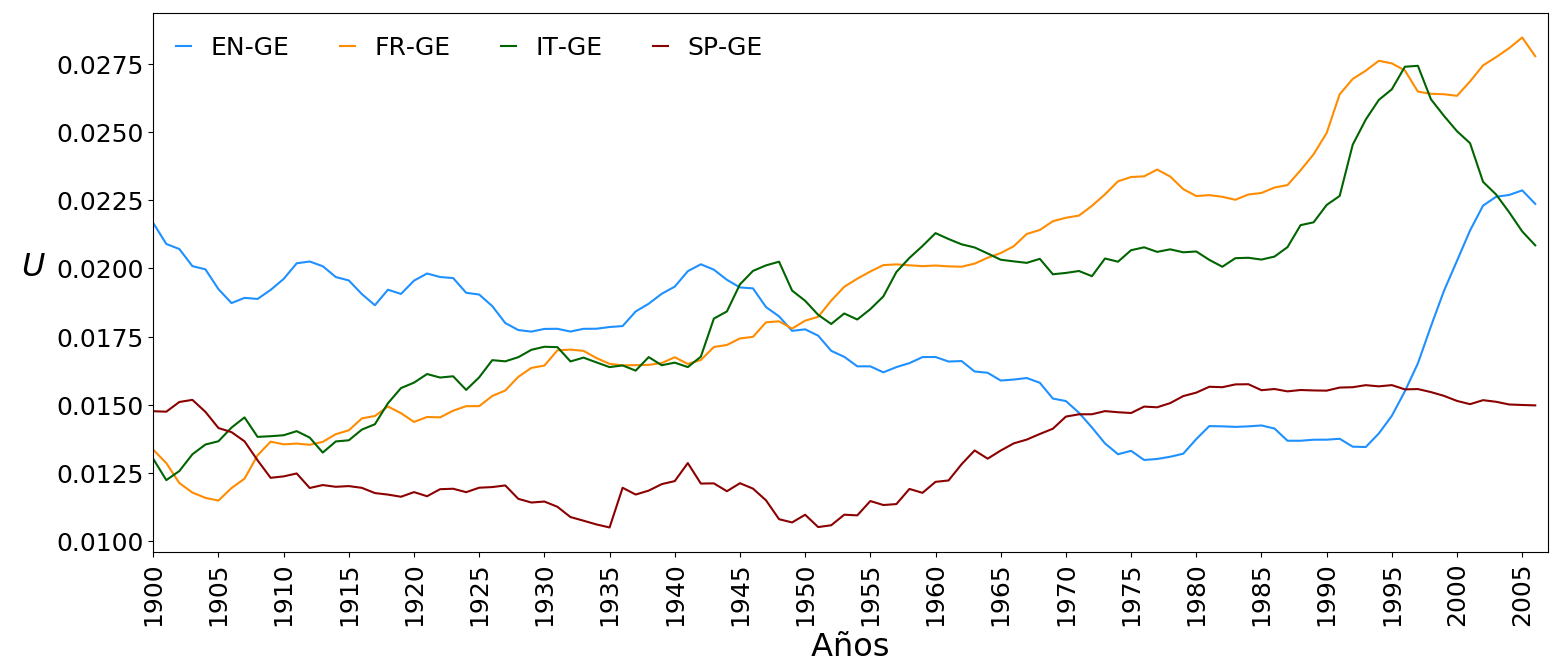
\includegraphics[scale=.36]{PF2_S2_GE.png}
	\label{fig.ST_b_GE}
	\caption{Los demás en el alemán. Cada lengua ha tenido un periodo de  crecimiento posterior a 1950, mostrando al alemán como un idioma susceptible (al menos en la literatura) donde los demás idiomas han impactado y perdurado.}
\end{figure}


\clearpage


La característica principal de los términos en alemán  en los demás idiomas  son principalmente personajes germano-parlantes que sobresalieron en algún ámbito; siendo además los encontrados en los préstamos nuevos, \textit{Hitler}, \textit{Marx}, \textit{Einstein}, \textit{Freud}, \textit{Engels}, \textit{Heidegger}, \textit{Mozart}, \textit{Hegel} y  \textit{Nietzsche}. 

Como idioma receptor, el alemán adoptó palabras de diferentes campos, tecnológicos y de desarrollo por parte del inglés,  religiosos  por el francés, históricos en el italiano y médicos por el español.  Cada idioma presentó un periodo de crecimiento posterior a 1950  o a la segunda guerra mundial, donde al ser vencido alemania, el idioma tuvo que adaptarse a las tendencias donde los demás destacaban. 

\clearpage
\subsection{Italiano}

\begin{figure}
	\centering
	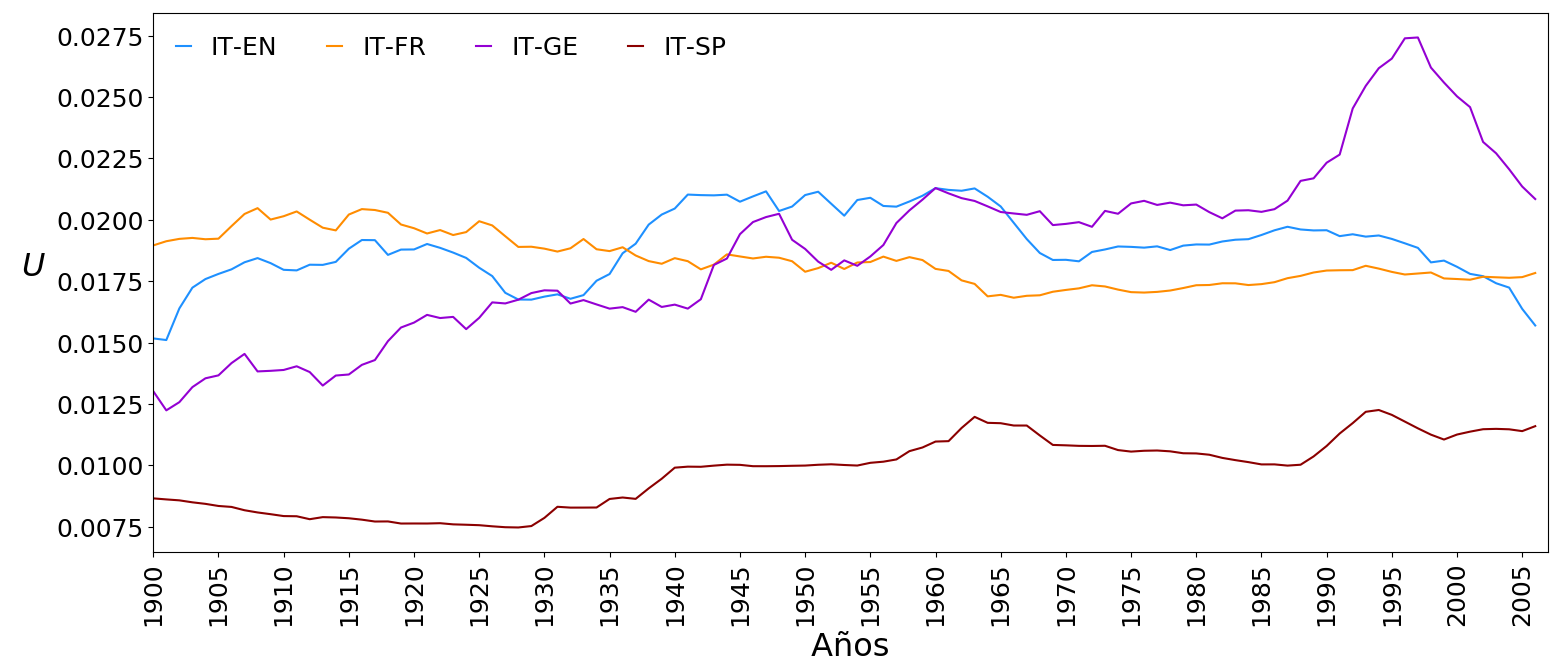
\includegraphics[scale=.36]{PF1_S2_IT.png}
	\label{fig.ST_a_IT}
	\caption{El italiano en los demás. A pesar de ser fonéticamente similares y de provenir de la familia de las lenguas romances,  el español persiste en ser el idioma con menor uso de italiano. La migración italiana a los Estados Unidos posterior a la primera guerra mundial coincide con el aumento en el inglés. }
\end{figure}
		
\begin{figure}[h!]
	\centering
	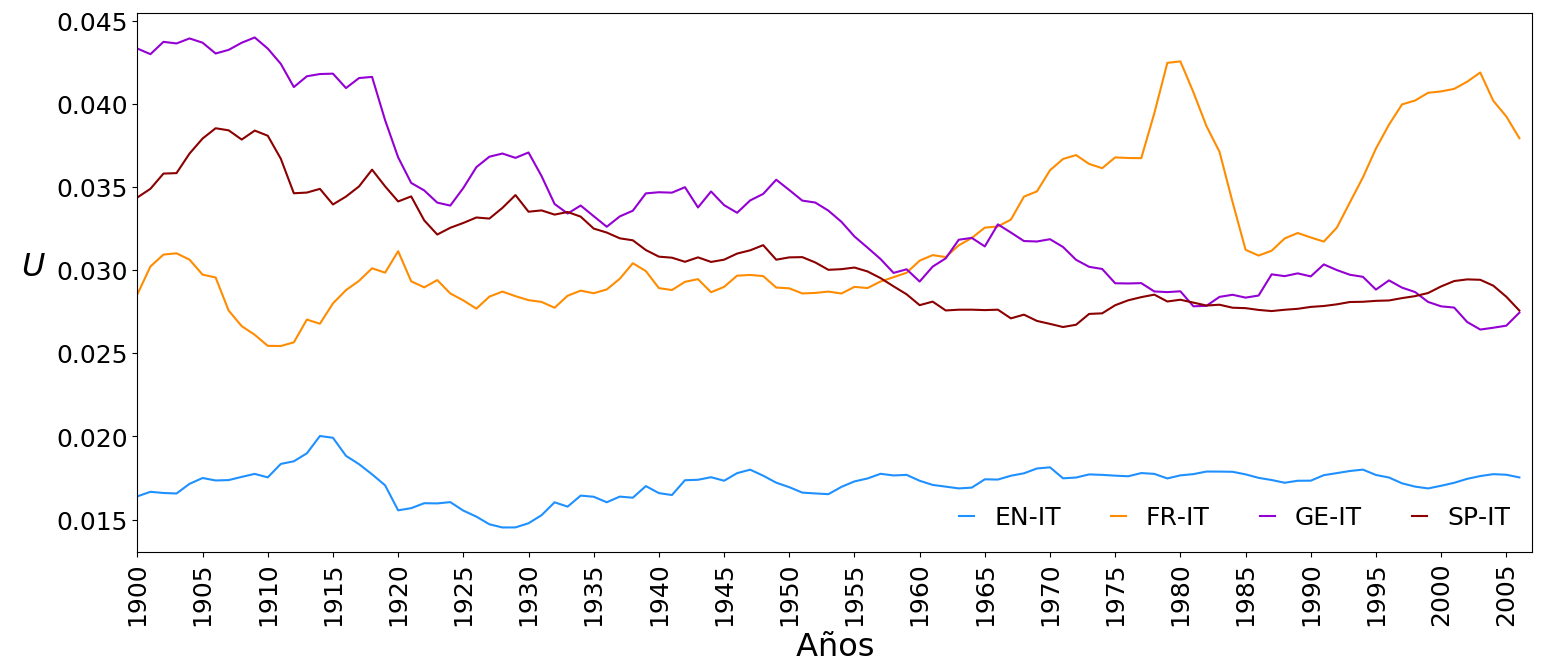
\includegraphics[scale=.36]{PF2_S2_IT.png}
	\label{fig.ST_b_IT}
	\caption{Los demás en el italiano. La proximidad geográfica  entre italia con países cuya lengua es el francés y el alemán ayudó a incrementar el uso de estos en el italiano. A pesar de que el inglés se difundió como un idioma universal para la comunicación, su uso en el italiano no ha mostrado un incremento considerable en todo el siglo XX. }
\end{figure}

\clearpage


El uso del italiano se vio caracterizado en la segunda mitad del siglo por la constante aparición y ascenso en rango de \textit{Mussolini}, siendo el personaje más relevante en el siglo pasado cuya lengua materna es el italiano.  Salvo por Mussolini, los demás prestamos italianos presentes en las otras lenguas no se lograron asociar a un único campo, sin embargo esto muestra la diversidad de temas en los cuales el italiano fue relevante, como términos políticos \textit{sociale}, \textit{liberale}, religiosos \textit{santo}, \textit{suora}, \textit{cattedrale} o  bélicos \textit{battaglia}, \textit{regime}.

El sentido inverso al considerar el tipo de palabras que utiliza el italiano de los demás idiomas, es igualmente variado por parte del ingles son conceptos ligados a la tecnología, por el francés a la industria vitivinícola, con el alemán a personajes relevantes de esta lengua,  términos que ya se han mencionado. Finalmente entre la variedad de palabras que toma del español se encuentran nombres de países o ciudades hispanohablantes \textit{México}, \textit{Chile}, \textit{Argentina}, \textit{Montevideo} o \textit{Peru}. 

\clearpage
\subsection{Español}

\begin{figure}[h!]
	\centering
	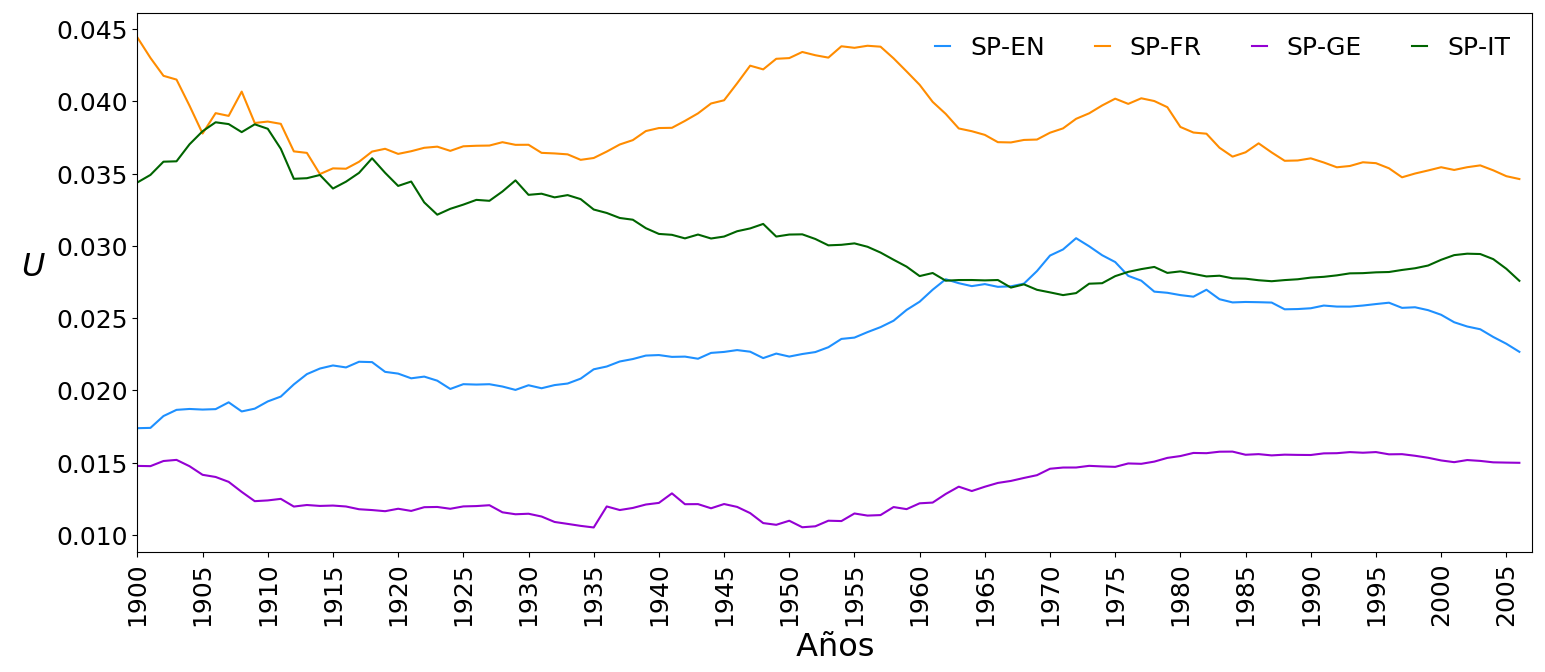
\includegraphics[scale=.36]{PF1_S2_SP.png}
	\label{fig.ST_a_SP}
	\caption{El español en los demás. Los idiomas que más emplean español son aquellos con los que comparte una relación etimológica, francés e italiano por ser lenguas romances y con el ingles al tener este idioma una base de palabras grecolatinas.     }
\end{figure}
		
\begin{figure}[h!]
	\centering
	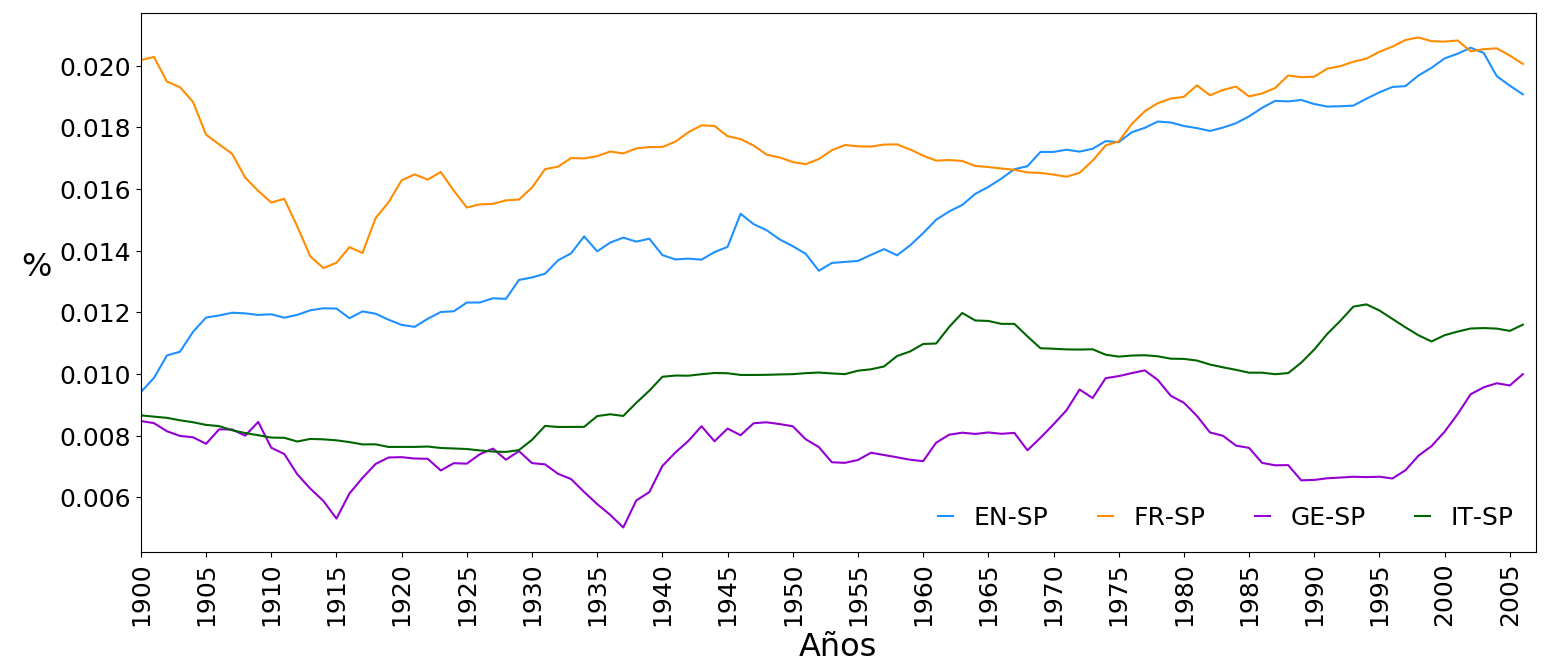
\includegraphics[scale=.36]{PF2_S2_SP.png}
	\label{fig.ST_b_SP}
	\caption{Los demás en el español.  Durante el último siglo, el contenido francés e inglés ha aumentado en el español siendo su uso equiparable, el surgimiento del inglés como el idioma universal y la relación etimológica con el francés  hacen posible los incrementos.}
\end{figure}

\clearpage

Entre los gráficos del apéndice 1, referentes al uso entre el español y un determinado idioma, se observo que el uso de los del español en los demás idiomas es mayor que el uso de los otros en él.  Ya se han comentado las características principales de las palabras interfieren en el uso, destacando el ámbito de la medicina, \textit{terapia}, \textit{lepra}, \textit{tumor}, \textit{syphilis}, \textit{virus} o \textit{renal}. Con ellos se infiere la productividad y la importancia de la medicina en países de lengua española antes de 1900; incluso en lenguas como el alemán se encontraron este tipo de préstamos. 


En las discusiones anteriores, se ha mencionado el tipo de palabras que los idiomas aportan,  en el caso de las contribuciones al español,   estas siguen la misma tendencia; del ingles los préstamos son de carácter tecnológico y del desarrollo industrial, del alemán son apellidos de personajes destacados en un campo especifico, mientras que del francés y el italiano son de condición religiosa y con una raiz etimológica grecolatina. 


\newpage
\section{Comentarios y complementos del método}


El determinar la influencia entre idiomas a través del uso de los préstamos, ha mostrado primeramente que el idioma que mas cantidad de palabras tiene en otro no siempre es el más utilizado,  radicando el mayor uso en aquel idioma cuyas préstamos tengan menores rangos en la lista de un receptor. 

En todo el siglo XX y la primer década del XXI, el inglés y el alemán han sido los idiomas más cambiantes en los papeles de origen y receptor respectivamente.
El inglés al ser el que más creció en tres idiomas (francés, alemán y español), complementando los resultados del capitulo anterior, al ser el idioma que más palabras nuevas exportó.  El alemán como el receptor donde los diferentes orígenes aumentaron su usó tras la segunda guerra mundial; el uso ha sido semejante a los préstamos nuevos, ha sido el receptor que más recibió. 

Ambos análisis se complementan,  el idioma más influyente ha aportado más palabras nuevas y aquellas que se van acumulando resultan las de mayor incremento en el uso. El idioma más influenciado recibió la mayor cantidad de palabras nuevas y el uso que han tenido los demás ha sido también el del mayor incremento. 

Por el momento sólo es posible describir que originó las variaciones en el uso o en la cantidad de nuevas palabras, no es posible predecir como se comportaran los idiomas en el futuro, ya que la principal característica que  hace fluir a las palabras entre idiomas han sido los eventos, reflejado en que las palabras de su campo semántico  se muevan a diferentes idiomas y continúen apareciendo o desapareciendo tras el suceso. 

Una mejor información de como los eventos alteran a los idiomas se podría extraer si se compararán las características de los prestamos con  datos de los países de alguna habla como lo pueden ser  el crecimiento economizo, el producto interno bruto, la alfabetización, la mortalidad, las migraciones de personas, entre otros.








      % ~20 páginas - Explicar el problema en específico que se va a resolver, la metodología y experimentos/métodos utilizados
\chapter{Eliminación de palabras}


Los capítulos anteriores se han enfocado en tratar a las migraciones de palabras como consecuencias de eventos donde  las lenguas están involucradas. La clasificación de los $n$-grams en palabras funcionales y palabras de contenido, y la posterior eliminación de las palabras funcionales, facilitó encontrar las relaciones con los eventos y establecer una cuantificación para la influencia entre idiomas (llamada uso), pero ¿qué sucedería con esta cantidad si se realizaran otras reglas para eliminar ciertas palabras?

Esta interrogante ha llevado a la construcción de un nuevo algoritmo que limite a las palabras,  reduciendo el conjunto de las migraciones y obteniendo nuevos valores del uso entre idiomas.  Elegidos una pareja de idioma origen \textit{A} e idioma receptor \textit{B}, el proceso es el siguiente. 


\begin{enumerate}
	
	\item Se toma la lista de los préstamos acumulados de \textit{A} en \textit{B},  este conjunto se denotará como \textbf{conjunto original}.
		
	\item Se escogen de forma aleatoria un conjunto de letras (desde una hasta diez), y se descartan de los préstamos acumulados a todas las palabras cuya primer letra sea alguna de las elegidas; siendo este nuevo grupo el \textbf{conjunto reducido}.
	
	\item Se establece un tercer grupo designado como \textbf{conjunto residuo}, conformado por todas las palabras eliminadas del conjunto original.  La unión del reducido y el residuo es el original. 
	
	\item En los tres conjuntos se emplea la ecuación \ref{ec.fuso}, para encontrar el uso de \textit{A} en \textit{B}. 	
	 
\end{enumerate}

La intención de estas alteraciones no es desaparecer el conjunto de las migraciones sino el reducirlas  y comparar el uso entre el conjunto original y el reducido.  Para poder decir que tanto ha cambiado el uso entre idiomas en los dos conjuntos, se utilizará el coeficiente de determinación $R^{2}$. 

El primer criterio importante sera tomar el uso en el conjunto original como verdadero(ya que con el se establecieron los resultados del capítulo anterior) identificando sus valores a lo largo del tiempo $t$ como $O_{t}$, si los valores de uso en el conjunto reducido se denotan como  $v_{t}$ y el promedio de ellos es $\bar{v}$, entonces   el coeficiente de determinación queda definido como:
 
\begin{equation}
 \label{ec.dif_uso}
 R^{2} = 1 - \sum_{t} \frac{ \left( v_{t}- O_{t} \right)^{2}  }{ \left( v_{t} - \bar{v} \right)^{2} }
\end{equation}

Se define el concepto \textbf{conservación del uso} para aquellos pares de conjuntos donde el uso no cambie a pesar de las omisiones; la conservación es favorable si $R^{2}$ es próximo a 1.  Si la conservación no es favorable, es indicio de que para el idioma las palabras que fueron eliminadas son las más relevantes. 

\section{Características de las eliminaciones}

El proceso anterior se realizó cuatrocientas veces por cada pareja de idiomas, obteniendo en cada uno un valor de $R^{2}$. Tras los múltiples descartes, se distinguieron las siguientes características al graficar el uso del conjunto original y del reducido. 


\begin{itemize}
	
	\item Valores iguales. Punto a punto el conjunto reducido empalma al original, siendo las gráficas indistinguibles. La conservación del uso se da en todo el intervalo de tiempo. 
	
	\item Diferencia de alturas. Ambas gráficas muestran el mismo comportamiento, sin embargo existe una diferencia casi constante entre el uso original y el reducido. En este caso se dirá que el uso también se conserva ya que ambas graficas tienen los mismos valores sólo que están desfasados. 
	
	\item Alteraciones por periodos.  Presenta periodos donde el uso de ambos conjuntos son completamente diferentes. La conservación se da por periodos de tiempo e incluso puede ser inexistente.

	
\end{itemize}

Para ilustrar las caracterizaras antes mencionadas, se exponen algunas graficas obtenidas, representado el uso del conjunto original con un trazo continuo, mientras que el uso en el conjunto reducido  es una serie de puntos. En cada grafica se especifica que idiomas se están tratando así como el conjunto de letras con las cuales se hicieron las eliminaciones. 


\begin{figure}[h!]
	\centering
	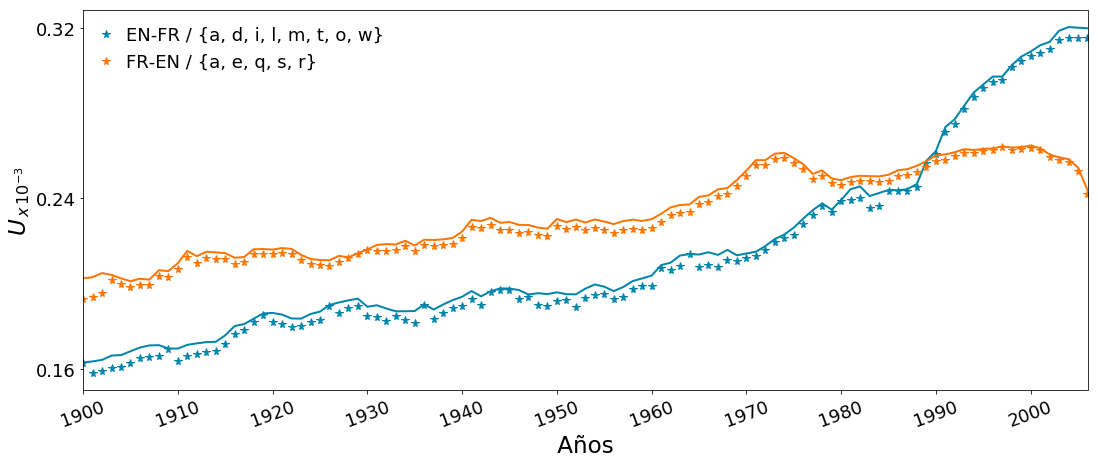
\includegraphics[scale=.38]{OM1.png}
	\label{fig.OM1}
	\caption{En ambas parejas de idiomas hay conservación del uso durante todo el siglo XX, al presentar valores iguales en el inglés-francés y  diferencia de alturas en el francés-inglés.}
\end{figure}


\begin{figure}[h!]
	\centering
	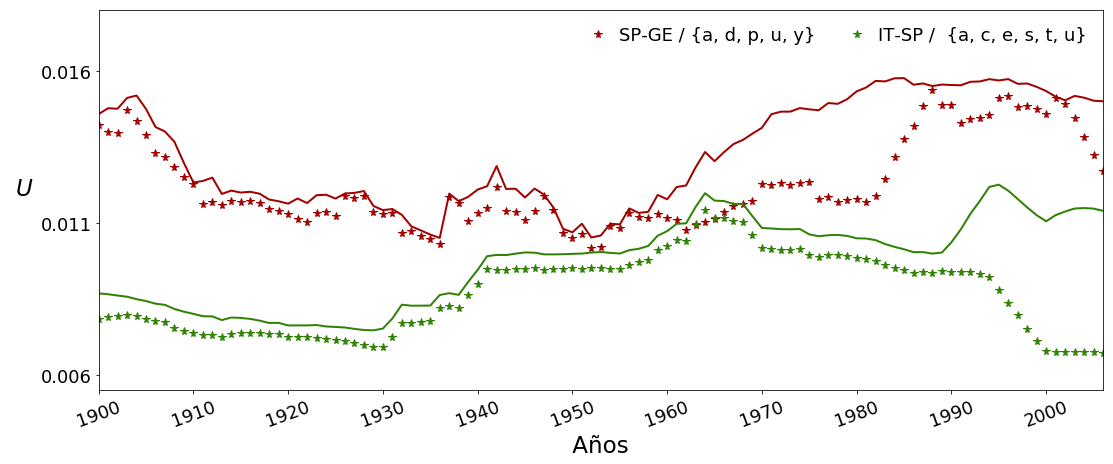
\includegraphics[scale=.38]{OM2.png}
	\label{fig.OM2}
	\caption{La conservación para el español-alemán no existió durante los años de 1960 a 1990,  correspondiendo a una alteración por periodos. Para el italiano-español el uso se conservo  en la mayor parte del siglo al existir una diferencia de alturas, en los últimos años se caracteriza por una alteración.}
\end{figure}


\begin{figure}[h!]
	\centering
	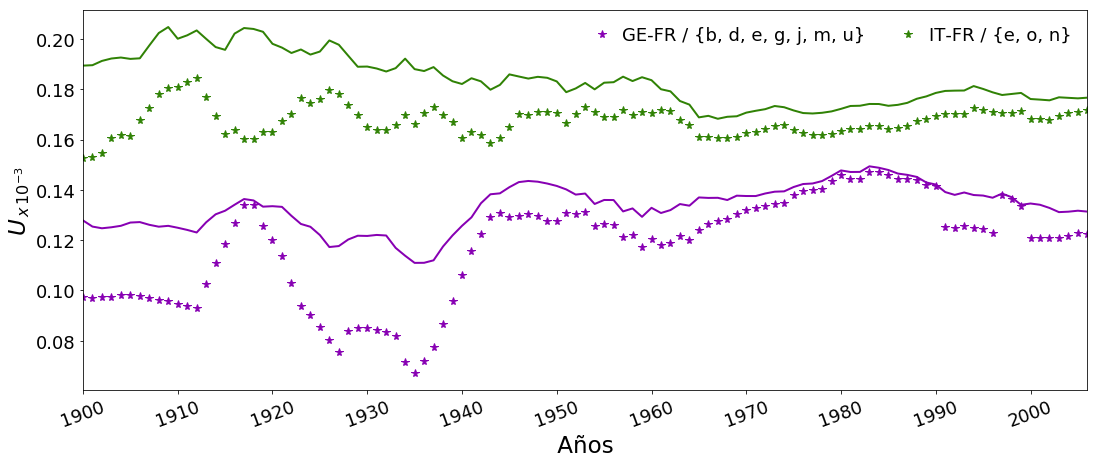
\includegraphics[scale=.38]{OM3.png}
	\label{fig.OM3}
	\caption{ En el italiano-francés la diferencia de alturas comienza a reducirse tras avanzar en los años, por lo que hay conservación. El alemán-francés  presenta las tres características,  valores iguales  en 1918, alrededor de 1980 y antes del 2000,  alteraciones entre 1920 y 1940, y deferencia de alturas  en los años restantes; en promedio durante todo el siglo XX el uso fue conservado, aunque en este caso la conservación dependerá del periodo tratado.}
\end{figure}


La característica del uso no siempre será la misma tras una nueva elección de letras, sin embargo  es posible decir de manera general si un idioma se conserva.  Para todas las repeticiones, se promedio el valor de $R^{2}$ por cada pareja de idiomas, y a la vez por cada idioma origen.  Los resultados de la tabla \ref{tab.conservacion} muestran de manera general si el idioma origen se conserva, así como con cuales receptores existieron más y menos cambios. 



\begin{table}[h!]
	\centering
	\begin{tabular}{cccc}
		\textbf{}         & \textbf{$R^{2}$} & \textbf{\begin{tabular}[c]{@{}c@{}}más \\ cambios\end{tabular}} & \textbf{\begin{tabular}[c]{@{}c@{}}menos \\ cambios\end{tabular}} \\
		\textbf{inglés}   & 0           & 0                                                               & 0                                                                 \\
		\textbf{francés}  & 0           & 0                                                               & 0                                                                 \\
		\textbf{alemán}   & 0           & 0                                                               & 0                                                                 \\
		\textbf{italiano} & 0           & 0                                                               & 0                                                                 \\
		\textbf{español}  & 0           & 0                                                               & 0                                                                
	\end{tabular}
	\caption{xxxx}
	\label{tab.conservacion}
\end{table}



\section{Comentarios del método}

El realizar diferentes elecciones para restringir a las palabras que conforman los prestamos de un idioma en otro, mostró desde el punto de vista estadístico que no importan cuales elementos conforman el corpus, la propiedad del uso es la misma, ya que individualmente los valores de uso de una única palabra pueden variar en los años del análisis y ser distintos a los de otra palabra, sin embargo al tratar a todo el conjunto, el uso se comporta de la misma  manera, sin importar los valores individuales de los elementos que lo conforman. 







            % ~5 páginas - Resumir lo que se hizo y lo que no y comentar trabajos futuros sobre el tema
\chapter{Diversidad de Rango}

Los primeros análisis se enfocaron en buscar hechos relevantes que propiciaron las migraciones de palabras,  siendo oportuna la información histórica.  El capítulo anterior busco ver a cada idioma como un conjunto “universal” donde las propiedades que lo caracterizan  son comunes en cada uno y siguen siendo válidas a pesar de reducir los elementos que los componen al extraer palabras. 

En esta sección se buscará entender cómo son las variaciones de palabras a  lo largo del tiempo, para ello  se enfocara el estudio a cuantificar que tan diferentes son las listas de los préstamos de un idioma en otro,  ya que estas listas están ordenadas por rango, (donde el rango más bajo es la palabra más común en ese año y la de rango más alto la menos utilizada)  una misma palabra puede ocupar distintos cargos en diferentes años,  o  para un mismo rango existe una diversidad de palabras que lo ocupan, esta idea es más adecuada ya hay palabras que no  aparecen en todos los años del análisis,  sin embargo en todos las listas  hay palabras hasta cierta posición (rango).   

La propuesta de la diversidad de rango ha utilizada en idiomas y en deportes [XXXX], siendo útil para mostrar características comunes de los conjuntos donde es medida.  El algoritmo para llegar a la diversidad se propuso en [XXX], y se describe de la siguiente manera:


\begin{enumerate}
	
	\item Se fijan un año inicial $t_{o}$ y uno final $t_{o}$, construyendo un intervalo de años a evaluar $\Delta\,t = t_{f}- t_{o}$.
	
	\item Se toma el primer rango de todos los años en el intervalo y se cuenta el número de palabras que son distintas en ese rango. Esta cantidad será la diversidad para el rango uno.
	
	\item Se prosigue con el segundo rango y se vuelve a contar cuántas palabras son diferentes en todo el periodo de tiempo.  Con ello se obtiene la diversidad para el rango dos. 
	
	\item Ya que las listas de préstamos de un idioma en otro no son homogéneas en cantidad, el procedimiento anterior se repetirá hasta el rango mínimo que poseen todas las listas,  así se asegura tener una homogeneidad en el tamaño.
	
	\item Se normalizan  los valores dividiendo cada resultado entre el número de años comprendidos del intervalo $\Delta\,t$, obteniendo  la diversidad de rango $d(k)$.
	
	
\end{enumerate}


Antes de mostrar los resultados, se espera  que los valores de $d(k)$ sean cercanos a cero cuando  para un rango $k$, las cantidad de palabras que ocupan ese rango sea menor. En caso de que la diversidad sea cercana a uno,  significa que hay una mayor cantidad de palabras que ocupan el rango $k$. 


Tras graficar el rango contra la diversidad, se observó que en todas las combinaciones (a pesar de que algunas tuvieran más datos)  la tendencia de la diversidad  se asemeja a una función de distribución cumulativa logarítmica  normal, la cual depende del rango $k$, y la desviación estándar $\sigma$.

\begin{equation}
	\label{ec.cumulativa}
	F(k) = \Phi \left ( \frac{ln(k)}{\sigma} \right )\,\,\,\,k\geq 0; \sigma \geq 0
\end{equation}

Donde $\Phi$ es la función cumulativa de la distribución normal, que ademas del rango y la desviación estándar, depende del promedio $\mu$.

\begin{equation}
	\label{ec.distribucionnormal}
	\Phi(t) = \frac{1}{\sigma\sqrt{2\pi}} \int_{-\infty}^{t}  e^{ \frac{ - \left ( x-\mu \right )^{2}}{2\sigma^2}  } dx	
\end{equation}


\newpage
\subsubsection*{Ajuste de Datos }


Se intentó ajustar los puntos de la diversidad con esta distribución, sin embargo al ser pocos los rangos (la mayor cantidad de rangos en cualquier combinación fue de 250),  la curva descrita  no ajusta correctamente;  si se tuvieran mayor cantidad de rangos (1000 o 1000) del orden de $10^{3}$ o $10^{4}$ el ajuste es más preciso.  Para solucionar este problema se propuso hacer un ajuste lineal con la función logarítmica  de la siguiente forma:


\begin{enumerate}
	\item Se propone una función para la diversidad $d(k)$ de la forma
	
	\begin{equation}
	\label{ec.ajuste}
	y(k) =  \alpha \, ln(k) + \beta
	\end{equation}
	
	\item Al realizar los cambios de variable $\hat{Y} = y(k)$ y $X = ln(k)$, se obtiene una ecuación lineal para $k$.
	$$ \hat{Y} =  \alpha X + \beta$$
	
	\item Para encontrar los parámetros $\alpha$ y $\beta$, se utilizó el método de mínimos cuadrados, minimizando la suma de los cuadrados de los errores.  
	
	\item Conocidos los valores de $X$, la diversidad $Y$ y la cantidad de valores $n$,  se calcularon los valores muestrales de las medias ($\mu_{X}$ y $\mu_{Y}$), las varianzas ($\sigma^{2}_{X}$ $\sigma^{2}_{Y}$)  y la covarianza de las dos variables  $\sigma_{XY}$.
	
	$$ \bar{X} = \frac{1}{n} \sum_{i=1}^{n} X_{i} $$
	
	$$ \bar{Y} = \frac{1}{n} \sum_{i=1}^{n} Y_{i} $$
	
	$$ \sigma^{2}_{X} = \frac{1}{n} \sum_{i=1}^{n} \left (X_{i} -\bar{X}\right )^{2} $$
	
	$$ \sigma^{2}_{Y} = \frac{1}{n} \sum_{i=1}^{n} \left (Y_{i} -\bar{Y}\right )^{2} $$
	
	$$ \sigma_{XY} = \frac{1}{n} \sum_{i=1}^{n} \left (X_{i} - \bar{X}\right )  \left (Y_{i} - \bar{Y} \right ) $$
	
	\item Así los parámetros se expresan como
	
	$$ \alpha = \frac{\sigma_{XY}}{\sigma^{2}_{X}} $$
	
	$$ \beta = \bar{Y} - \alpha \bar{X}$$
	
	\item Calculados cada punto del ajuste (\ref{ec.ajuste}) $y_{i}$ y los valores calculados de diversidad $f_{i}$, para comprobar que tan adecuado es el ajuste se obtiene el coeficiente de determinación $R^{2}$.
	
	\begin{equation}
	\label{ec.rcuadrado}
	R^{2} = \frac{\sigma_{XY}}{\sigma^{2}_{X} \sigma^{2}_{Y}} \,\, = \,\, 1- \frac{\sum_{i=1}^{n} \left( y_{i} - f_{i}\right)^{2} }{\sum_{i=1}^{n} \left (y_{i} -\bar{Y}\right )^{2}}
	\end{equation}
	
	
	 
\end{enumerate}


Valores de $R^{2}$ próximos a 1 indicarán que existe una relación lineal ( en este caso logarítmica por el cambio de variable) exacta entre las dos variables

Las posteriores gráficas corresponden a las diferentes combinaciones entre idiomas orígenes y los receptores donde se calculó la diversidad de rango y el ajuste correspondiente.  Por cada conjunto de gráficas se muestra una tabla con los diferentes parámetros, la media $\mu$, la desviación estándar $\sigma$, el rango minimo donde se buscó la diversidad $k_{min}$, los parámetros del ajuste $\alpha$ y $\beta$  y el coeficiente de determinación $R^{2}$.
 
\newpage

\begin{figure}[h!]
	\centering
	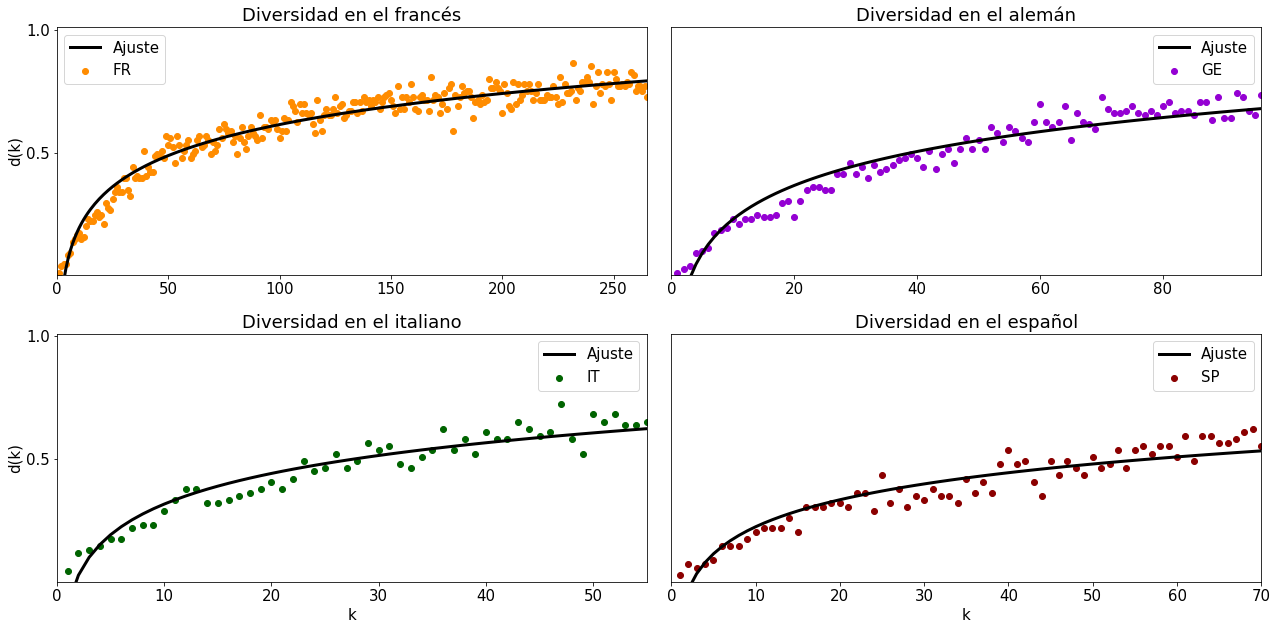
\includegraphics[width=15cm, height=6.8cm]{Cap_6/DR_EN.png}
	\label{fig.DR_EN}
	\caption{Diversidad de rango del inglés en los demás.}
\end{figure}


\begin{table}[h!]
	\centering
	\begin{tabular}{ccccccc}
		\textbf{}                & \textbf{$\mu$} & \textbf{$\sigma$} & \textbf{$k_{min}$} & \textbf{$\alpha$} & \textbf{$\beta$} & \textbf{$R^{2}$} \\
		\textbf{inglés-francés}  & 0.61           & 0.18                & 265                   & 0.18           & -0.23         & 0.94        \\
		\textbf{inglés-alemán}   & 0.49           & 0.19                & 96                    & 0.19           & -0.23         & 0.92        \\
		\textbf{ingles-italiano} & 0.45           & 0.17                & 55                    & 0.17           & -0.10         & 0.91        \\
		\textbf{ingles-español}  & 0.38           & 0.15                & 70                    & 0.15           & -0.14         & 0.88       
	\end{tabular}
	\caption{Parámetros de la diversidad del inglés en los demás.}
	\label{tab.DR_EN}
\end{table}



\newpage

\begin{figure}[h!]
	\centering
	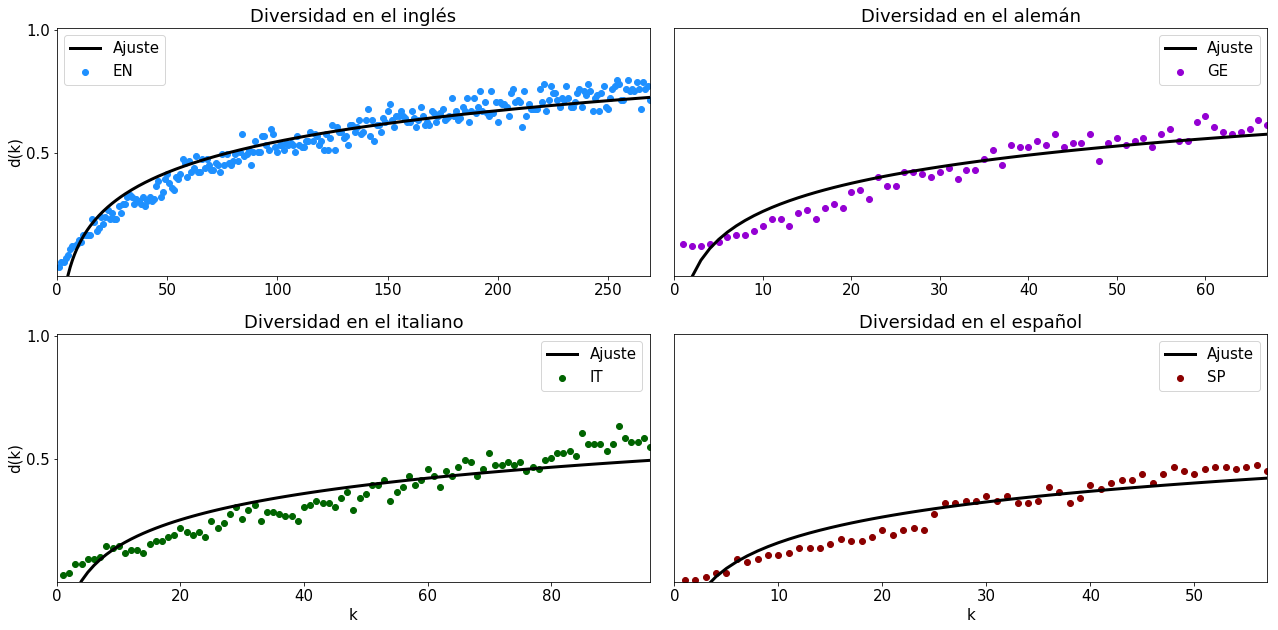
\includegraphics[width=1 \textwidth, scale = .38]{Cap_6/DR_FR.png}
	\label{fig.DR_FR}
	\caption{Diversidad de rango del francés en los demás.}
\end{figure}


\begin{table}[h!]
	\centering
	\begin{tabular}{ccccccc}
		\textbf{}                & \textbf{$\mu$} & \textbf{$\sigma$} & \textbf{$k_{min}$} & \textbf{$\alpha$} & \textbf{$\beta$} & \textbf{$R^{2}$} \\
		\textbf{francés-inglés}  & 0.55           & 0.18                & 269                   & 0.18           & -0.29        & 0.93        \\
		\textbf{francés-alemán}   & 0.42           & 0.16                & 67                    & 0.17           & -0.12         & 0.87        \\
		\textbf{francés-italiano} & 0.35           & 0.16                & 96                    & 0.15           & -0.21         & 0.83        \\
		\textbf{francés-español}  & 0.28           & 0.14                & 57                    & 0.15           & -0.19         & 0.86       
	\end{tabular}
	\caption{Parámetros de la diversidad del francés en los demás.}
	\label{tab.DR_FR}
\end{table}


\newpage

\begin{figure}[h!]
	\centering
	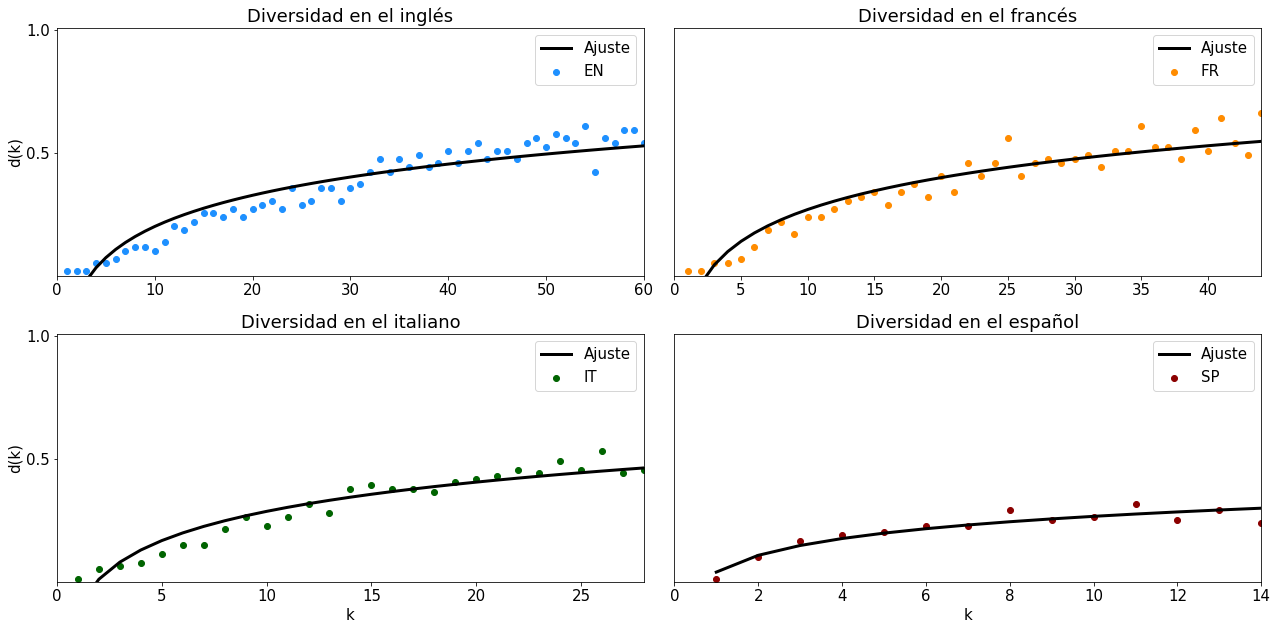
\includegraphics[width=1 \textwidth, scale = .38]{Cap_6/DR_GE.png}
	\label{fig.DR_GE}
	\caption{Diversidad de rango del alemán en los demás.}
\end{figure}


\begin{table}[h!]
	\centering
	\begin{tabular}{ccccccc}
		\textbf{}                & \textbf{$\mu$} & \textbf{$\sigma$} & \textbf{$k_{min}$} & \textbf{$\alpha$} & \textbf{$\beta$} & \textbf{$R^{2}$} \\
		\textbf{alemán-inglés}  & 0.35          & 0.17                & 60                   & 0.18           & -0.22        & 0.88        \\
		\textbf{alemán-francés}   & 0.37           & 0.17                & 44                    & 0.19           & -0.16         & 0.89        \\
		\textbf{alemán-italiano} & 0.31           & 0.15                & 28                    & 0.17           & -0.11         & 0.91        \\
		\textbf{alemán-español}  & 0.22          & 0.08                & 14                    & 0.10           & -0.04         & 0.89       
	\end{tabular}
	\caption{Parámetros de la diversidad del alemán en los demás.}
	\label{tab.DR_GE}
\end{table}


\newpage

\begin{figure}[h!]
	\centering
	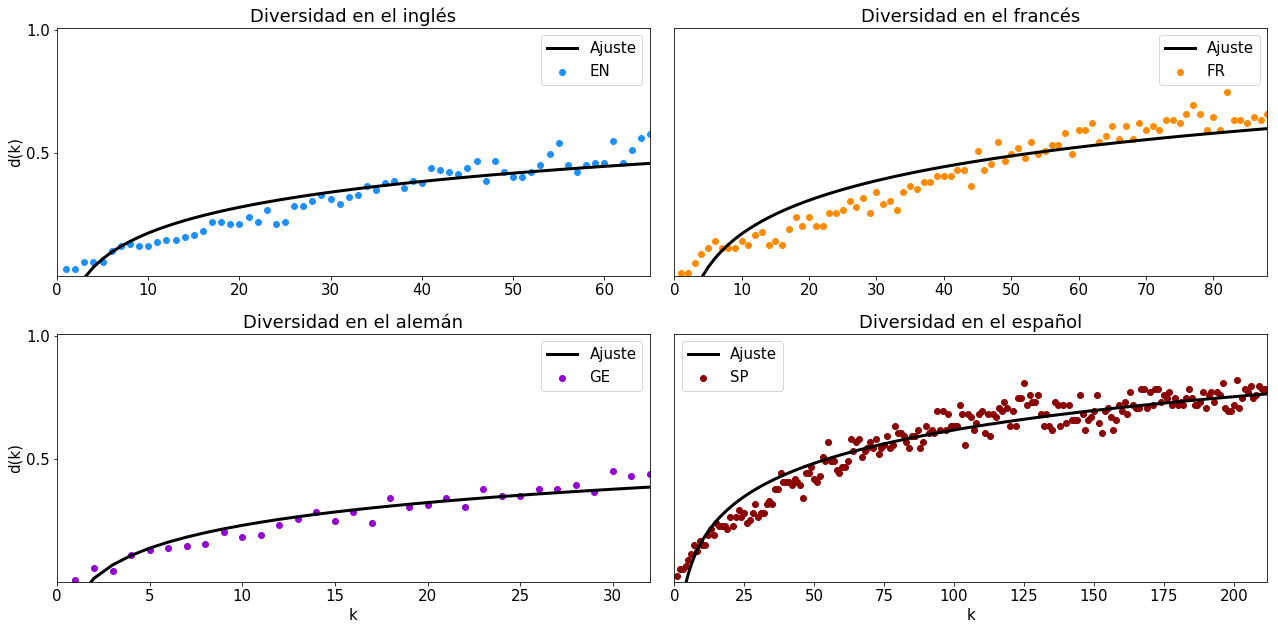
\includegraphics[width=1 \textwidth, scale = .38]{Cap_6/DR_IT.png}
	\label{fig.DR_IT}
	\caption{Diversidad de rango del italiano en los demás.}
\end{figure}


\begin{table}[h!]
	\centering
	\begin{tabular}{ccccccc}
		\textbf{}                & \textbf{$\mu$} & \textbf{$\sigma$} & \textbf{$k_{min}$} & \textbf{$\alpha$} & \textbf{$\beta$} & \textbf{$R^{2}$} \\
		\textbf{italiano-inglés}  & 0.31          & 0.15                & 66                   & 0.15           & -0.18        & 0.86        \\
		\textbf{italiano-francés}   & 0.41           & 0.20                & 88                    & 0.20           & -0.28         & 0.85        \\
		\textbf{italiano-alemán} & 0.26           & 0.12                & 32                    & 0.13           & -0.08         & 0.91        \\
		\textbf{italiano-español}  & 0.22          & 0.19                & 212                    & 0.20           & -0.28         & 0.92       
	\end{tabular}
	\caption{Parámetros de la diversidad del italiano en los demás.}
	\label{tab.DR_IT}
\end{table}


\newpage

\begin{figure}[h!]
	\centering
	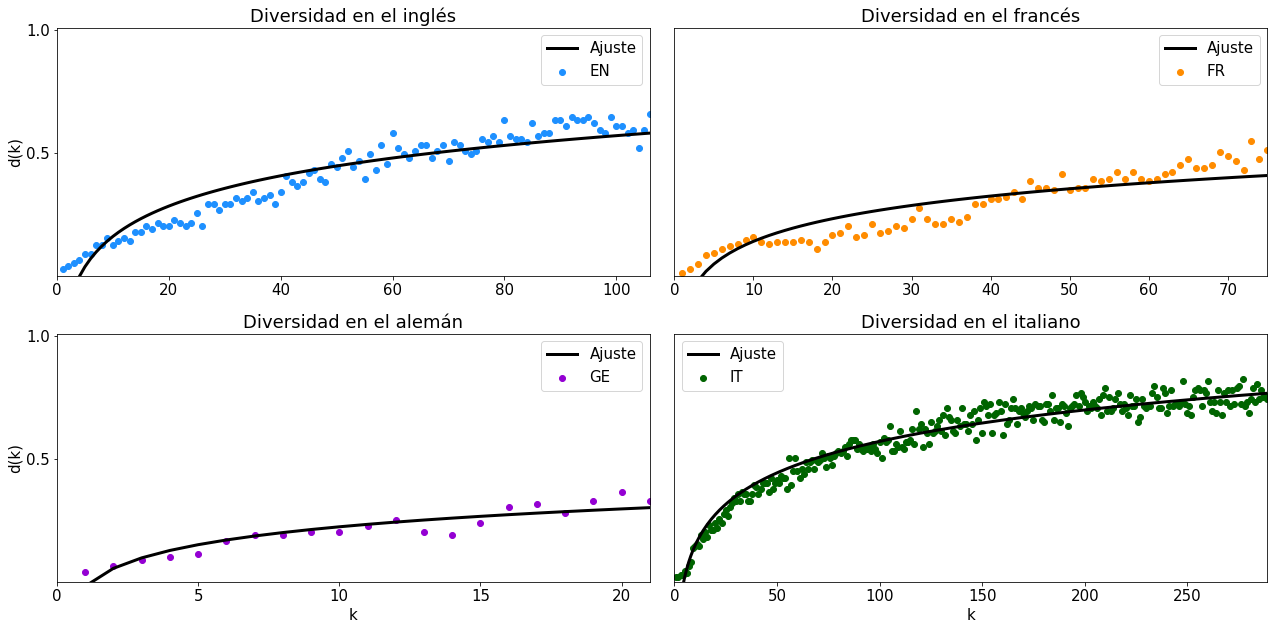
\includegraphics[width=1 \textwidth, scale = .38]{Cap_6/DR_SP.png}
	\label{fig.DR_SP}
	\caption{Diversidad de rango del español en los demás.}
\end{figure}


\begin{table}[h!]
	\centering
	\begin{tabular}{ccccccc}
		\textbf{}                & \textbf{$\mu$} & \textbf{$\sigma$} & \textbf{$k_{min}$} & \textbf{$\alpha$} & \textbf{$\beta$} & \textbf{$R^{2}$} \\
		\textbf{español-inglés}  & 0.41          & 0.18                & 106                   & 0.18           & -0.25        & 0.87        \\
		\textbf{español-francés}   & 0.28           & 0.14                & 75                   & 0.13           & -0.17         & 0.79        \\
		\textbf{español-alemán} & 0.21           & 0.09                & 21                    & 0.11           & -0.02         & 0.86        \\
		\textbf{español-italiano}  & 0.22          & 0.18                & 289                    & 0.18           & -0.28         & 0.95       
	\end{tabular}
	\caption{Parámetros de la diversidad del español en los demás.}
	\label{tab.DR_SP}
\end{table} 

\chapter{Conclusiones}

En el presente trabajo, se ha tratado de estimar una forma para cuantificar la influencia que un idioma ejerce sobre otro,  a partir de la construcción de dos métodos. 

En el primero método al contar las palabras nuevas, se expuso que las palabras que migran de un idioma a otro son parte de un mismo campo semántico, y las migraciones ocurren tras un suceso que tiene relación con el campo semántico. Con ello, se refleja la influencia que tiene un idioma en determinadas áreas.  

El segundo método para cuantificar la influencia, por medio del uso de un idioma en otro, mostró que las palabras migrantes que continuamente son empleadas por los demás idiomas, también son parte de un mismo campo semántico. Además, estas descienden su rango (aumentan su frecuencia), en los años posteriores al evento que las hizo migrar. 

Con ambos métodos, se concluyó que las áreas donde un idioma es más influyente, y cuyas palabras son continuamente empleadas, son en el inglés la guerra, la economía, la tecnología, la política y la globalización; en el francés la guerra, la Revolución Francesa, la religión y la industria vitivinícola; en el alemán la guerra y los apellidos de personajes germano parlantes que destacaron el algún área académica; en el italiano  la guerra, la política y la religión; y en el español la medicina y la cultura de los países Latinoamericanos. 

En la parte estadística del trabajo, se destaca que las palabras migrantes de cada pareja de idiomas, siguen una regla común si estas se ordenan de acuerdo a su frecuencia de aparición, y es que en cada año, la cantidad de distintas palabras que pueden ocupar un lugar en el ordenamiento, aumentará de forma logarítmica conforme se avancen lugares en el ordenamiento. 

En el ultimo capitulo del trabajo, se trataron de justificar los resultados, pese al escaso rigor lingüístico que se tuvo. En esta justificación, se mostró que a pesar que una palabra (o un conjunto de ellas) no pertenezca con exactitud a un idioma,  el uso de un idioma en otro no se ve alterado si está es excluida del conjunto. La eliminación de palabras, ejemplifica que mientras se considere a las palabras como un conjunto,  estas mantendrán sus características, sin importar cuantos elementos conformen el conjunto. 






%%%%%%%%%%%%%%%%%%%%%%%%%%%%%%%%%%%%%%%%%%%%%%%%%%%%%
%                   APÉNDICES                       %
%%%%%%%%%%%%%%%%%%%%%%%%%%%%%%%%%%%%%%%%%%%%%%%%%%%%%
\appendix

% this file is called up by thesis.tex
% content in this file will be fed into the main document
\chapter{Complementos}
% top level followed by section, subsection

\section{Lectura de listas}
\label{lectura.listas}
 
Las listas hechas para los préstamos nuevos \cite{prestamos_nuevos} o acumulados \cite{prestamos_acumulados} de un idioma origen \textit{A} en un receptor \textit{B},  se encuentran ordenadas por cada año de estudio (1740-2009), y a la vez, las palabras listadas se ordenaron de forma descendente en la frecuencia $f$ y ascendente en rango $k$,  es decir en la lista del año $t$, la palabra con rango $k=1$ es la más frecuente,  la correspondiente a $k=2$ es la segunda más frecuente, para $k=3$ es la tercera más frecuente y así sucesivamente para todas las palabras en ese año. 


Si para el año $t$  se encontraron $n$ cantidad de palabras, cuyas frecuencias cumplen que $f_{1} > f_{2} > f_{3} >  \dots > f_{n-1} > f_{n}$,  entonces el ordenamiento es el siguiente. 

\begin{table}[h!]
	\centering
	\begin{tabular}{ccc}
		\multicolumn{3}{c}{\textbf{Año $t$}}        \\
		Rango $k$     & Palabra    & Frecuencia $f$    \\
		1             & pal 1      & $f_{1}$            \\
		2             & pal 2      & $f_{2}$             \\
		3             & pal 3      & $f_{3}$              \\
		$\vdots$      & $\vdots$   & $\vdots$         \\
		$\vdots$      & $\vdots$   & $\vdots$         \\
		$n-1$         & pal $n-1$  & $f_{n-1}$             \\
		$n$           & pal $n$    & $f_{n}$          
	\end{tabular}
\end{table}


Para su mejor lectura y evitar confusiones con los números,  se omitieron las frecuencias en los listados. 








\section{Gráficas de palabras acumuladas entre dos idiomas}
\label{palabras.acumuladas.apendice}

\begin{figure}[h!]
	\centering
	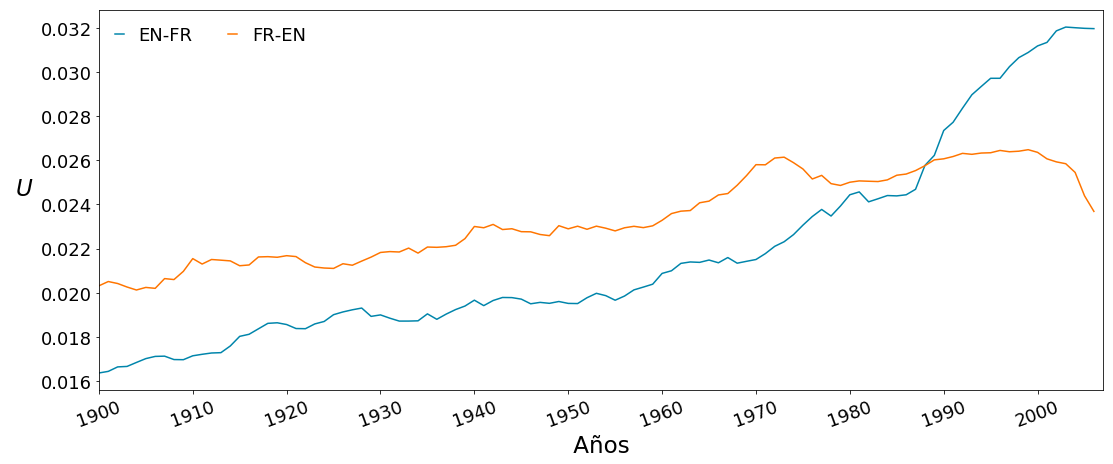
\includegraphics[scale=.38]{UOR_1EN.png}
	\label{fig.U_EF}
	\caption{Palabras acumuladas entre el inglés y el francés}
\end{figure}


\begin{figure}[h!]
	\centering
	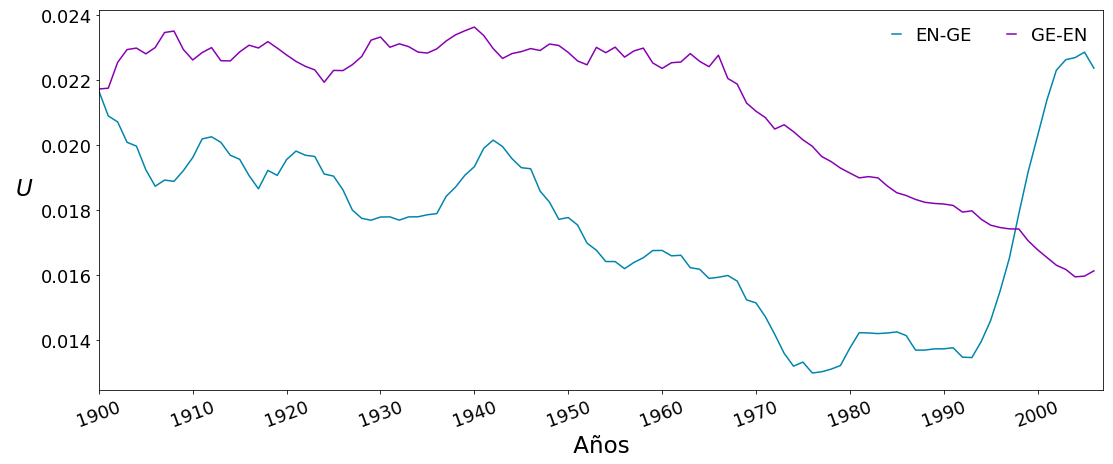
\includegraphics[scale=.38]{UOR_2EN.png}
	\label{fig.U_EG}
	\caption{Palabras acumuladas entre el inglés y el alemán}
\end{figure}


\begin{figure}[h!]
	\centering
	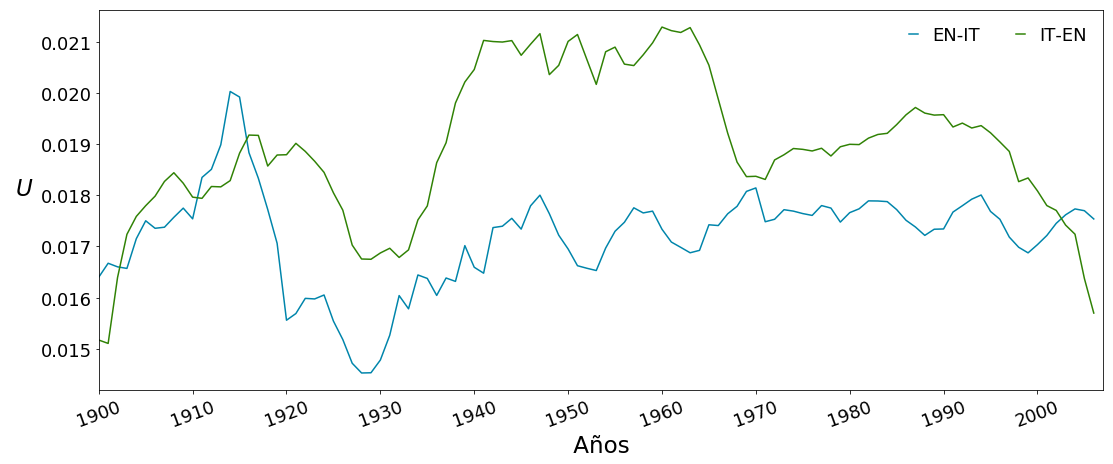
\includegraphics[scale=.38]{UOR_3EN.png}
	\label{fig.U_EI}
	\caption{Palabras acumuladas entre el inglés y el italiano}
\end{figure}

\begin{figure}[h!]
	\centering
	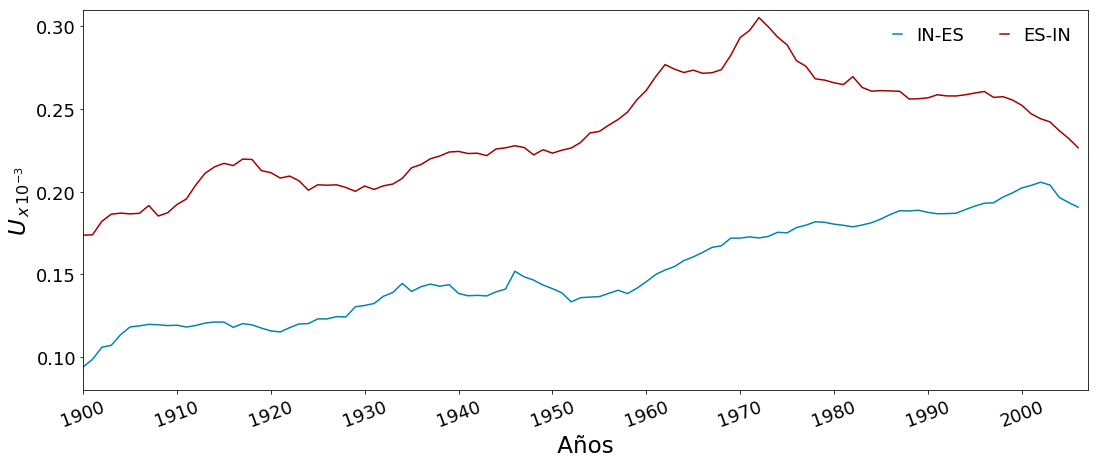
\includegraphics[scale=.38]{UOR_4EN.png}
	\label{fig.U_ES}
	\caption{Palabras acumuladas entre el inglés y el español}
\end{figure}

\begin{figure}[h!]
	\centering
	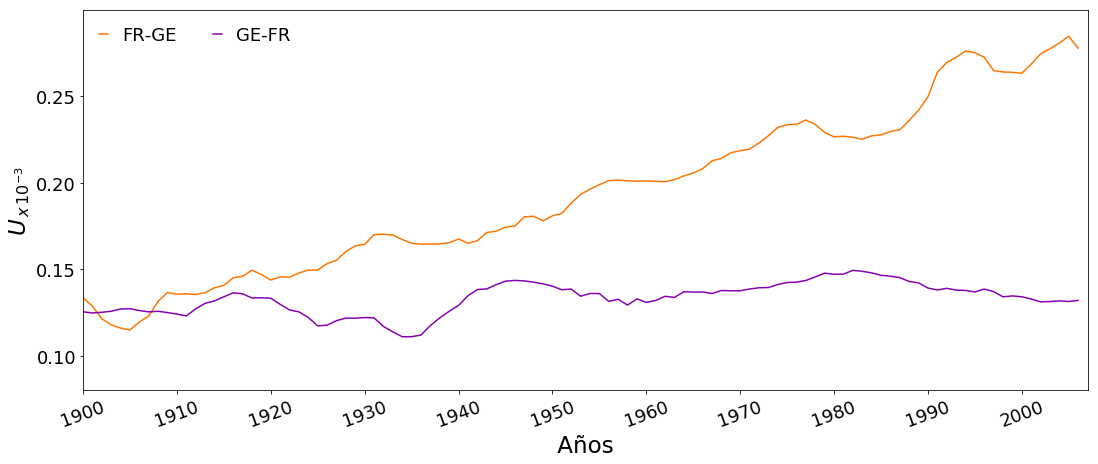
\includegraphics[scale=.38]{UOR_1FR.png}
	\label{fig.U_FG}
	\caption{Palabras acumuladas entre el francés y el alemán}
\end{figure}

\begin{figure}[h!]
	\centering
	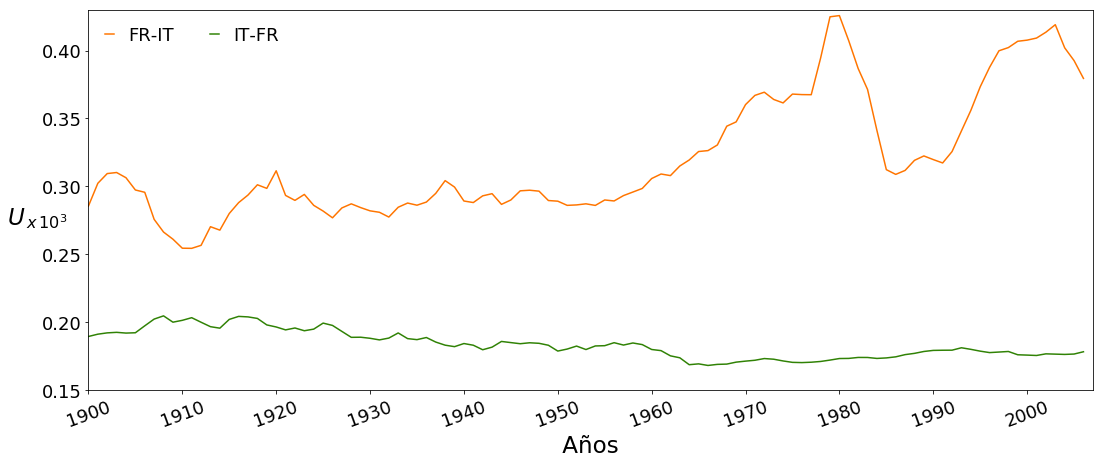
\includegraphics[scale=.38]{UOR_2FR.png}
	\label{fig.U_FI}
	\caption{Palabras acumuladas entre el francés y el italiano}
\end{figure}

\begin{figure}[h!]
	\centering
	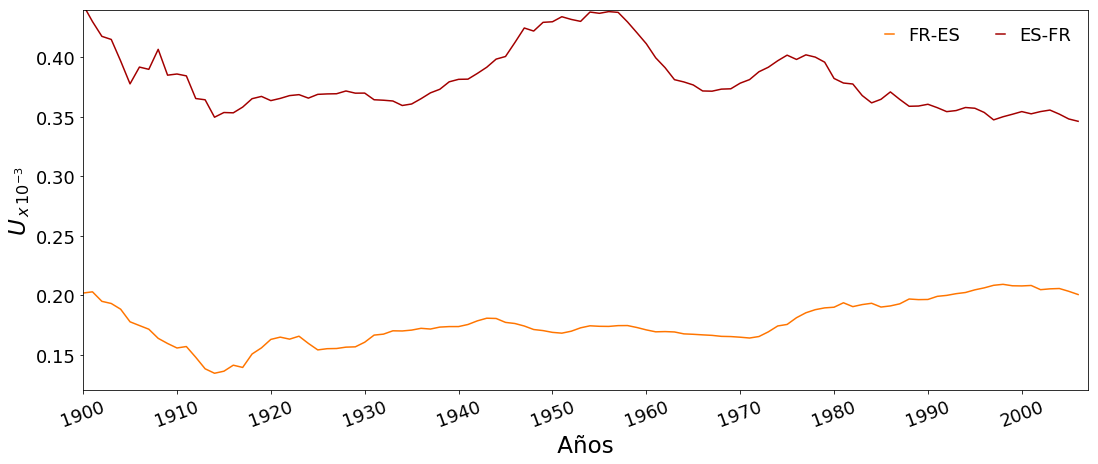
\includegraphics[scale=.38]{UOR_3FR.png}
	\label{fig.U_FS}
	\caption{Palabras acumuladas entre el francés y el español}
\end{figure}



\begin{figure}[h!]
	\centering
	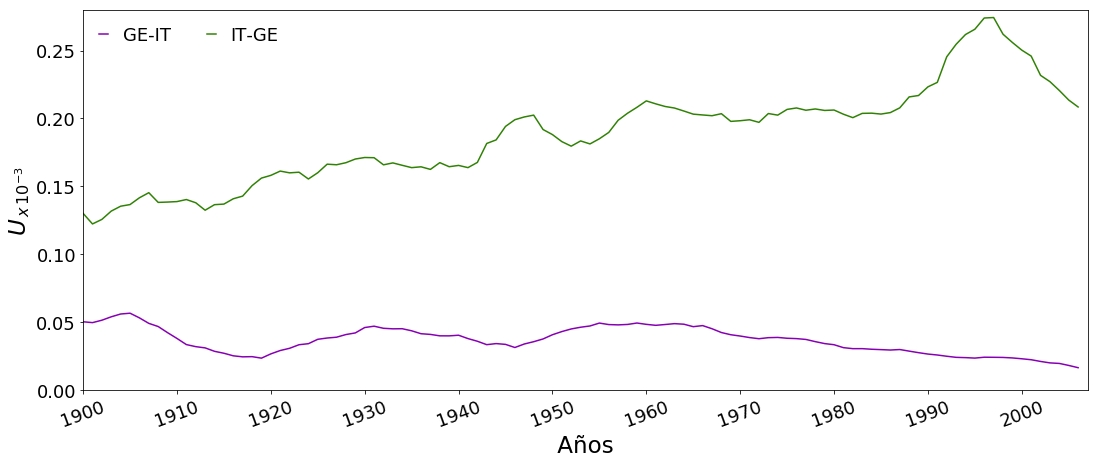
\includegraphics[scale=.38]{UOR_1GE.png}
	\label{fig.U_GI}
	\caption{Palabras acumuladas entre el alemán y el italiano}
\end{figure}


\begin{figure}[h!]
	\centering
	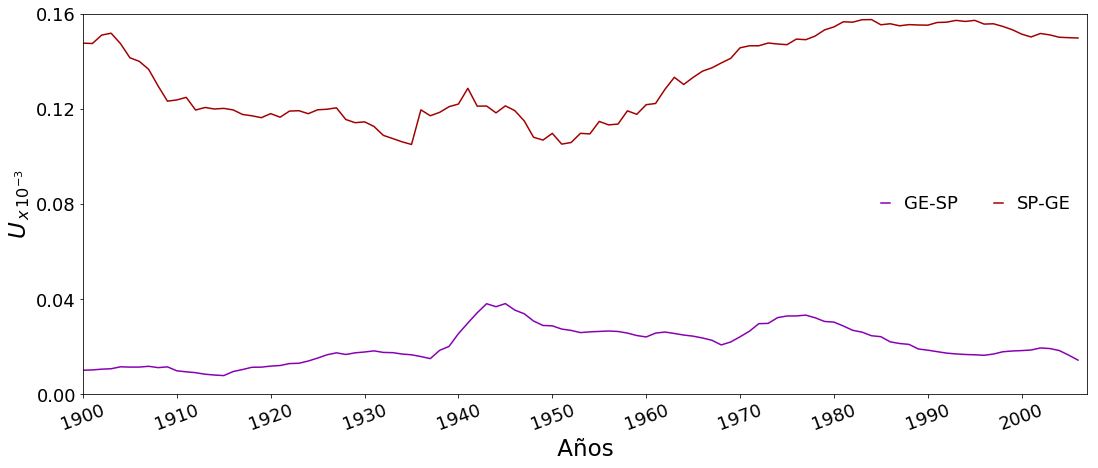
\includegraphics[scale=.38]{UOR_2GE.png}
	\label{fig.U_GS}
	\caption{Palabras acumuladas entre el alemán y el español}
\end{figure}


\begin{figure}[h!]
	\centering
	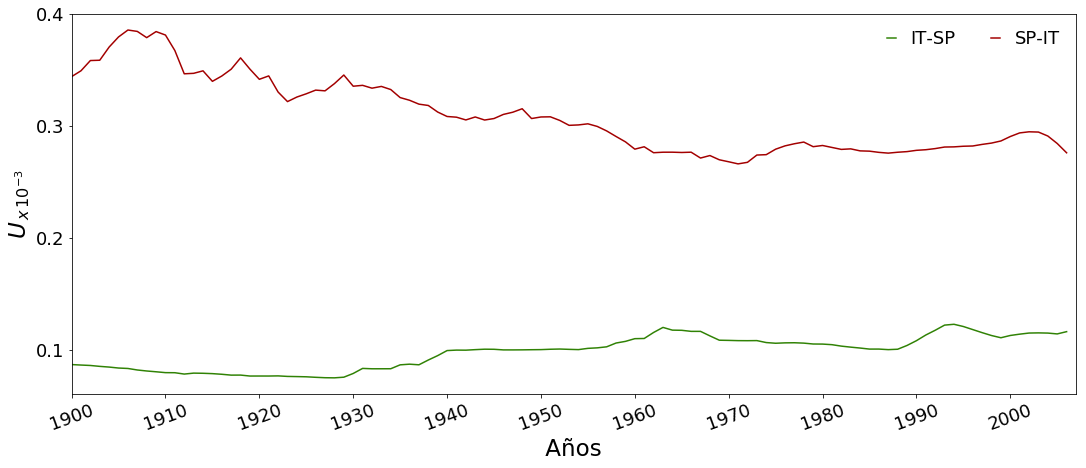
\includegraphics[scale=.38]{UOR_1IT.png}
	\label{fig.U_IS}
	\caption{Palabras acumuladas entre el italiano y el español}
\end{figure}

%\section{Eliminación de palabras}
%\label{eliminacion.completa.apendice}


               % Colocar los circuitos, manuales, código fuente, pruebas de teoremas, etc.

%%%%%%%%%%%%%%%%%%%%%%%%%%%%%%%%%%%%%%%%%%%%%%%%%%%%%
%                   REFERENCIAS                     %
%%%%%%%%%%%%%%%%%%%%%%%%%%%%%%%%%%%%%%%%%%%%%%%%%%%%%
% existen varios estilos de bilbiografía, pueden cambiarlos a placer
%\bibliographystyle{apalike} 
%\bibliographystyle{unsrt}
% otros estilos pueden ser abbrv, acm, alpha, apalike, ieeetr, plain, siam, unsrt

%El formato trae otros estilos, o pueden agregar uno que les guste:
%\bibliographystyle{Latex/Classes/PhDbiblio-case} % title forced lower case
%\bibliographystyle{Latex/Classes/PhDbiblio-bold} % title as in bibtex but bold
\bibliographystyle{Latex/Classes/PhDbiblio-url} % bold + www link if provided
%\bibliographystyle{Latex/Classes/jmb} % calls style file jmb.bst

\bibliography{Bibliografia/referencias}             % Archivo .bib

\end{document}